% !TeX root = ../../book.tex

\chapter[关系与模算术]{关系与模算术:构造集合与整数性质的证明}\label{ch:chapter06}

% !TeX root = ../../../book.tex
\section{引言}

在我们建立起坚实的数学术语和概念基础之后,你可能会好奇接下来要讨论什么!就像我们之前严格化了数学归纳法的概念一样,在接下来的两章中,我们将进一步探讨一个你可能已经直观理解但还未精确定义的概念:\textbf{函数}。

为此,我们将从\textbf{关系}开始讨论,进而探讨\textbf{等价关系},这将有助于我们研究集合的一些性质。特别地,我们将利用集合 $\mathbb{Z}$ 上的等价关系来陈述并证明许多有趣的整数性质。这将让我们有机会一览\textbf{数论}这个丰富多彩的领域。我们将通过陈述和证明一些有用的定理,并用它们解决一些有趣的问题来初探数论的王国。然后,我们将继续下一章,回到讨论函数的目标上来。

% !TeX root = ../../../book.tex

\subsection{目标}

以下简要说明本章在本书中的定位。我们将阐释先前内容如何发挥作用,阐述研究本章主题的动机,明确学习目标,并提示阅读时的关注重点。我们会先列出本章的核心目标及学成后应掌握的技能,后续章节将详细展开。学完本章后,请返回此处核验:你是否理解所有目标?能否阐述其重要性?能否定义相关术语?能否运用相关技术?

\textbf{学完本章后,你应该能够……}

\begin{itemize}
    \item 定义关系并给出多个例子。
    \item 定义并理解关系的各种属性,举例说明哪些关系具备或不具备这些属性。
    \item 研究已定义的关系,发现并证明其属性。
    \item 定义等价关系和等价类,并解释其重要性与意义。
    \item 研究已定义的等价关系,并对等价类进行分类。
    \item 利用整数集上的特定等价关系,陈述并证明数论中的有趣结论。
    \item 定义乘法逆元的概念,理解其在模算术中的意义,并应用该概念证明或证伪特定方程的解。
    \item 陈述并理解数论中的各种定理,应用这些定理解决问题。
\end{itemize}

% !TeX root = ../../../book.tex

\subsection{承上}

本章内容不像之前章节那样紧密关联,而是开启了本书的\emph{新篇章}。从现在起,我们将运用先前学到的所有数学知识探索新领域。此前的学习都是为此刻做准备:我们将提出复杂命题并用证明技巧加以论证,提供定义和定理,并期望你用这些工具证明其他命题。可以说,本章是对之前\emph{所有}章节的综合应用,我们将充分利用之前积累的知识、术语和经验!

% !TeX root = ../../../book.tex

\subsection{启下}

你可能在微积分中处理过函数(如微分与积分),在高中代数课上绘制过函数图像或求根,甚至在计算机科学中编写过递归算法。但尝试\emph{定义}函数本身是另一码事——如何向从未接触数学的人解释?如何向超智能外星人说明?若以数学归纳法般的严谨性表述,该怎么做?这并非易事。

为了深入理解\emph{函数}概念,我们需要先探讨\emph{关系}——一种比较集合元素的方法。通过大量例子了解其性质后,下一章将揭示函数本质是关系的特殊类型!讨论过程中,我们将探究关系属性,发现特定属性组合形成的重要性质。尤其将看到\emph{等价关系}自然生成集合\emph{划分},反之亦然。这一洞见将助力我们陈述并证明关于整数的关键结论。

% !TeX root = ../../../book.tex

\subsection{忠告}

本章将继续探讨抽象概念与严谨数学内容。若你对此类日益抽象的内容和语言感到不适,切勿认为它们``无关紧要''或``毫无用处''——这些概念将贯穿全书乃至整个数学领域!注意力涣散时请谨记这一点。建议做些学习笔记,理解定理后在书页边缘写下摘要;绘制示意图辅助理解案例或定理核心;遇到定义时记录典型示例与反例;阅读证明后梳理论证步骤,将概念``模块化''以便记忆。若对定义、定理或证明心存疑惑,请务必记录下来!向同学、助教或教授寻求解答。最重要的是,消化吸收这些抽象概念与论证需要\emph{时间},通过案例验证理解程度依然至关重要。若能向他人清晰解释某个概念,那说明你已经真正掌握了它。

\newpage
% !TeX root = ../../book.tex
\section{抽象(二元)关系}

% !TeX root = ../../../book.tex

\subsection{定义}

让我们直入主题,开始讨论关系。我们会先给出定义,然后提供一系列例子。

\begin{definition}
    设 $A, B$ 为集合。$A$ 和 $B$ 之间的\dotuline{关系}是由\dotuline{有序对}组成的集合,$R \subseteq A \times B$。对于元素 $a \in A$ 和 $b \in B$,当且仅当 $(a, b) \in R$ 时,我们说 $a$ 和 $b$ 是\dotuline{相关的}。

    集合 $A$ 称为\dotuline{定义域},集合 $B$ 称为\dotuline{值域}。集合 $R$ 称为\dotuline{关系集}。
    
    如果 $A = B$,我们称 $R$ 为 $A$ 上的关系。
\end{definition}

另一种常见的写法是用 $x \;R\; y$ 来表示 $(x,y) \in R$。当我们通过这种方式定义关系时,会坚持使用 $(x, y) \in R$ 来表示其基础集合结构。之后,我们有时会用一些符号来定义关系,比如 $x < y$ 或 $x \;\bigstar\; y$ 等等。

\begin{remark}
    我们这里定义的关系有时也叫\emph{二元关系},因为它涉及两个``输入'';集合 $R$ 是由\emph{有序对}组成的。

    我们可以将这个概念推广到\emph{三元关系}。也就是说,给定集合 $A,B,C$,我们可以定义 $R \subseteq A \times B \times C$ 为三元关系,当且仅当 $(a, b, c) \in R$ 时,$a,b,c$ 是相关的。我们还可以进一步推广到具有 $n$ 个``输入''的关系。不过,在本书中,我们只考虑\emph{二元关系},因此``\emph{关系}''一词将专指\emph{二元关系}。
\end{remark}

\begin{remark}
    关系 $R$ 通常通过确定 $A$ 和 $B$ 元素的某个\emph{性质}来定义(用变量命题 $P(a,b)$ 表示),并设定
    \[(a,b) \in R \iff P(a,b)\]
\end{remark}

\subsubsection*{示例}

\begin{example}
    设 $W=\{\text{英文单词}\}, L=\{\text{英文字母}\}$,定义关系 $R$ 如下:
    \[(w, \ell) \in R \iff w \text{以 } \ell \text{ 开头}\]
    则 $(\text{mathematics},\text{m}) \in R$ 且 $(\text{golf},\text{g}) \in R$,因为这些都是有效的单词,我们已经确定了它们的首字母。再来看一些反例,比如 $(\text{knowledge},\text{n}) \notin R$ 且 $(\text{you},\text{u}) \notin R$。此外 $(\text{zyzyxyqy},\text{z}) \notin R$,因为 $\text{zyzyxyqy} \notin W$。
\end{example}

$A = B$ 的情况经常出现,所以 $R$ 定义了同一集合中元素对之间的关系。下一个例子就是针对这种情况的。\\

\begin{example} \label{ex:example6.2.5}
    设 $A=B=\mathbb{Z}$,定义 $\mathbb{Z}$ 上的关系 $R$ 如下:
    \[(x, y) \in R \iff x \text{ 和 } y \text{ 具有相同的奇偶性}\]
    则 $(2,8) \in R, (-3, 7) \in R, (-99, -99) \in R$,但 $(1,2) \notin R, (0, -3) \notin R$,且 $(\pi, 0) \notin R$(因为 $\pi \notin \mathbb{Z}$)。
\end{example}

\begin{example} \label{ex:example6.2.6}
    定义 $\mathbb{R}$ 上的关系 $L$ 如下:
    \[(x, y) \in L \iff x < y\]
    则 $(-1, \pi) \in L$ 且 $(0, 100) \in L$,但 $(2, 2) \notin L$ 且 $(\pi, -1) \notin L$。
\end{example}

请注意,这里的对都是\emph{有序对}(我们可能会忘记这一点,因为 $A = B = \mathbb{R}$),所以元素的顺序很重要。确实,知道 $(x, y) \in L$ 并不一定意味着 $(y, x) \in L$。在上面这个例子中,这种情况实际上总是错误的!

回想一下,我们有时用 $x \;L\; y$ 来表示 $(x, y) \in L$,所以我们可以说 $-1 \;L\; \pi$ 但 $\pi \;\cancel{L}\; -1$,并且 $2 \;\cancel{L}\; 2$。

\subsubsection*{空关系}

\begin{remark}
    到目前为止,我们看到的例子在某种程度上都是有趣的关系。对于任意 $x,y \in R$,我们可以通过比较来判断 $x$ 是否小于 $y$。换句话说,我们看到的每个例子都是通过这样的方式定义的:对某性质 $P(a, b), (a, b) \in R \iff P(a, b)$ 为真。
\end{remark}

不过,关系不一定要这样定义。举个例子,我们知道对于任何集合 $S$,都有 $\varnothing \subseteq S$。因此,给定两个集合,我们总是可以通过 $\varnothing \subseteq A \times B$ 这一事实来定义一个\emph{平凡关系}。也就是说,\emph{平凡关系}是指没有任何元素相关的关系。这虽然看起来``无趣'',但它仍然符合关系的定义,所以我们也接受这种关系。

\subsubsection*{任何有序对的集合都是一个关系}

\begin{remark}
    给定集合 $A$ 和 $B$,任何子集 $R \subseteq A \times B$ 都定义了一个关系。然而,要找到一个能够描述这种关系的性质可能会非常困难,甚至是不可能的。

    比如 $A=\{1,3,5\}$ 且 $B=\{\bigstar, \heartsuit\}$,则我们可以定义 $A, B$ 上的关系
    \[R=\{(1,\bigstar), (5, \heartsuit)\}\]
    为什么 $1$ 与 $\bigstar$ 有关系?为什么 $3$ 不与任何元素有关系?这谁也说不清楚。这只是一个有序对的集合!从数学角度讲,这完全没有问题。
\end{remark}

\subsubsection*{相等关系}

\begin{example} \label{ex:example6.2.9}
    另一种在任意集合 $X$ 上定义关系的方法是定义相等关系。也就是说,如果 $(x, y) \in R \iff x = y$。需要注意的是,这种定义与集合 $X$ 的具体内容无关,只要它是一个\emph{集合}即可。
\end{example}

\subsubsection*{关系之间的相似之处}

\begin{example}
    假设 $S$ 是你班上学生的集合。定义 $S$ 和 $\mathbb{N}$ 之间的关系 $R_1$,如果 $(s, n) \in R_1$,那么表示学生 $s \in S$ 的年龄是 $n$ 岁。写出这个关系集的一些元素。

    现在,在集合 $S$ 内定义关系 $R_2$,如果 $(s, t) \in R_2$,那么表示学生 $s$ 和 $t$ 的年龄相同(以年为单位)。写出这个关系集的一些元素。

    比较关系 $R_1$ 和 $R_2$,它们是否以某种方式传达了关于集合 $S$ 的相同信息?为什么是或为什么不是?是否可以通过 $R_1$ 确定 $R_2$?反过来是否也可以?仔细思考这些问题,并尝试总结你的想法。我们马上将在下一小节中讨论这些问题,但现在先花点时间自己思考一下吧!
\end{example}

\subsubsection*{关系``编码''信息}

前面的例子旨在说明抽象关系的实际用途,并解释我们为什么要讨论它们(除了我们想要严格定义函数这一目标之外)。从某种意义上说,关系是一种``保存''两个集合或一个集合中元素信息的方法,是比较两个元素并判断它们是否满足某性质的一种手段。而在更广泛的意义上,关系可以提供关于集合元素在特定性质下表征的信息。

例如,在前面的例子中,关系 $R_1$ 告诉了我们更多关于集合 $S$ 元素的信息。确切地说,$R_1$ 告诉我们哪些人年龄相同:我们可以找到像 $(s, n)$ 和 $(t, n)$ 这样的对,它们的第二个值相同。同时,$R_1$ 还告诉我们具体年龄是多少:只需要查看这些对的第二个值即可。而 $R_2$ 则不行。知道 $(s, t) \in R_2$ 只告诉我们学生 $s$ 和学生 $t$ 年龄相同,却没有具体的年龄信息!从这个角度讲,$R_1$ 是一个``更好''的关系,因为它提供了更多的信息。

不过,$R_2$ 也有其优点!例如,它有一个很好的性质:如果 $(x, y) \in R_2$,那么 $(y, x) \in R_2$ 也必然成立。这个性质在 $R_1$ 中显然不成立,因为当 $(s, n) \in R_1$ 时,说 $(n, s) \in R_1$ 是没有意义的,因为顺序不匹配定义域和值域!那么这个性质是否使 $R_2$ 成为一个``更好''的关系呢?嗯,这要看具体情况以及我们想要编码和检索的信息类型。在某些情况下,你可能会选择使用 $R_1$,而在其他情况下,你可能会选择使用 $R_2$。

不过我们这里有点超前了!我们还不能详细解释这些性质的含义及其优缺点。然而,总的来说,我们对这些性质及其在给定集合的所有元素对中何时(或何时不)成立感兴趣。在下一小节中,我们将定义和探索几种常见的抽象关系性质。虽然不能保证任何关系都具备这些性质,但它们在数学和实际应用中已被证明是有趣和有用的。之后,我们将看到更多关系的例子,并讨论如何证明这些性质成立。在这个过程中,我们将培养处理关系的直觉,甚至弄清楚我们首先要证明的那些声明的类型!

% !TeX root = ../../../book.tex

\subsection{关系的性质}

我们先来定义几个性质。对于这些性质,每个关系要么满足,要么不满足。建议你逐一阅读每个性质,并尝试构建满足该性质的关系,然后再构建不满足该性质的关系。这将有助于你深入理解性质的本质及关系的运作方式。(也可尝试定义同时具有多种性质的关系!)定义完性质后,我们会提供典型示例,但请先尝试自己构思并分享有趣例子!

\subsubsection*{定义:集合上关系的性质}

这些性质涉及元素对顺序的\emph{颠倒}。给定 $(x, y) \in R$,我们可能会考虑 $(y, x)$;但定义域与值域要求 $(y, x) \in A \times B$。因此需要满足 $A \times B = B \times A$,而这仅当 $A = \varnothing$、$B = \varnothing$ 或 $A = B$ 时成立。(参考第 \ref{ch:chapter03} 章集合论中的证明!)由于 $A = \varnothing$ 和 $B = \varnothing$ 的情形通常不考虑,我们讨论这些性质时假设 $A = B$ 且 $A \ne \varnothing$,即定义在非空集合上的关系。

\begin{definition}
    设 $A$ 为集合,$R$ 为 $A$ 上的关系,即 $R \subseteq A \times A$。
    \begin{itemize}
        \item 若
            \[\forall x \in A \centerdot (x, x) \in R\]
            则称 $R$ 具有\dotuline{自反性}。即每个元素都与其自身相关。
        \item 若
            \[\forall x,y \in A \centerdot (x, y) \in R \implies (y,x) \in R\]
            则称 $R$ 具有\dotuline{对称性}。即比较的顺序无关紧要。
        \item 若
            \[\forall x, y, z \in A \centerdot [(x, y) \in R \land (y, z) \in R] \implies (x, z) \in R\]
            则称 $R$ 具有\dotuline{传递性}。即关系可以通过中间元素传递。
        \item 若
            \[\forall x, y \in A \centerdot [(x, y) \in R \land (y, x) \in R] \implies x = y\]
            则称 $R$ 具有\dotuline{反对称性}。即两个不同元素最多只能有一种关系,或者根本没有关系。为了理解为什么这是等价的陈述,观察上述条件陈述的逆否命题:
            \[\forall x, y \in A \centerdot x \ne y \implies [(x, y) \notin R \lor (y, x) \notin R]\]
    \end{itemize}
\end{definition}

需要注意的是,\emph{反对称性 (anti-symmetric)} 与\emph{非对称性 (asymmetric)}并不相同。通过逻辑结构和量词可验证差异:例如 $\mathbb{R}$ 上的 $\le$ 关系满足反对称性但不满足对称性,请思考其中缘由。

尝试寻找既满足\emph{反对称性}又满足\emph{对称性}的关系(这并不困难,我们之前已经提及过此类基本关系)。

% !TeX root = ../../../book.tex

\subsection{示例}

请再次尝试找出一些符合或不符合我们刚刚定义的四个性质的关系。下面展示一些定义在 $\mathbb{N}$ 上的典型例子,以提供具体参考。你也可以添加一些简单例子,比如定义在 $\mathbb{Z}$ 或 $\mathbb{R}$ 上的关系。\\

\begin{example}
    本例中,所有关系均定义在集合 $\mathbb{N}$ 上。
    \begin{itemize}
        \item 定义 $\mathbb{N}$ 上的关系 $R_1$
        \[(x, y) \in R_1 \iff x \text{\ 整除\ } y\]
        (即 $y$ 能被 $x$ 整除,或 $\exists k \in \mathbb{N}$ 使得 $y=kx$。该定义的严格陈述见定义 \ref{def:definition6.2.15}。)

        则 $R_1$ 具有自反性,因为 $x \mid x$,即 $x=1 \cdot x$。

        \textbf{整除关系具有自反性。}
        \item 定义 $\mathbb{N}$ 上的关系 $R_2$
        \[(x, y) \in R_2 \iff x \text{\ 和\ } y \text{\ 具有相同的奇偶性}\]
        则 $R_2$ 具有对称性,因为若 $x$ 和 $y$ 具有相同的奇偶性,则 $y$ 和 $x$ 也具有相同的奇偶性。

        \textbf{``相同奇偶性''关系具有对称性。}
        \item 定义 $\mathbb{N}$ 上的关系 $R_3$
        \[(x, y) \in R_3 \iff x < y\]
        则 $R_3$ 具有传递性,因为若 $x<y$ 且 $y<z$ 则 $x<y<z$,所以 $x<z$。

        \textbf{``$<$''关系具有传递性。}
        \item 定义 $\mathbb{N}$ 上的关系 $R_4$
        \[(x, y) \in R_4 \iff x \le y\]
        则 $R_4$ 具有反对称性,因为若 $x \le y$ 且 $y \le x$ 则 $x \le y \le x$,所以 $x=y$。

        \textbf{``$\le$''关系具有反对称性。}
    \end{itemize}
\end{example}

\begin{example}
    始终牢记:关系本质是一组有序对,不必通过性质定义。考虑以下例子:\\
    定义集合 $S=\{a,b,c\}$ 上的关系 $R$
    \[R = \{(a, a),(a, c),(b, c),(c, b)\}\]
    该关系
    \begin{itemize}
        \item 不具有自反性:\quad 因为 $(c,c) \notin R$
        \item 不具有对称性:\quad 因为 $(a, c) \in R$ 但 $(c, a) \notin R$
        \item 不具有传递性:\quad 因为 $(a, c) \in R$ 且 $(c, b) \in R$ 但 $(a, b) \notin R$
        \item 不具有反对称性:因为 $(b, c) \in R$ 且 $(c, b) \in R$ 但 $b \ne c$
    \end{itemize}
\end{example}

\begin{example}
    让我们练习使用略微不同的关系符号。注意:$x \;R\; y$ 等价于 $(x, y) \in R$。\\
    在班级同学集合 $S$ 上定义关系 $\bigstar$,对于任意 $x,y \in S$
    \[x \;\bigstar\; y \iff x \text{\ 和\ } y \text{\ 同一个月出生}\]
    我们声称该关系具有自反性、对称性、传递性。原因如下:
    \begin{itemize}
        \item 该关系具有\emph{自反性}:因为每个人当然与其自己同月出生(即 $x \;\bigstar\; x$)。
        \item 该关系具有\emph{对称性}:因为若 $x$ 与 $y$ 同月出生(即 $x \;\bigstar\; y$),则 $y$ 与 $x$(只是顺序不同!)当然也是同月出生(即 $y \;\bigstar\; x$)。
        \item 该关系具有\emph{传递性}:因为若 $x$ 与 $y$ 同月出生,且 $y$ 与 $z$ 同月出生,则 $x$ 与 $z$ 同月出生。我们只是在不断强调``相同''这个词的概念!
    \end{itemize}
    关于\emph{反对称性},这要看具体情况!班上是否有两个人同月出生?如果有,这种关系就不具有反对称性。然而,如果班上每个人都在不同月份出生,那么这种关系就具有反对称性,因为没有人会与别人有此关系,除了他自己!好好琢磨一下……
\end{example}


% !TeX root = ../../../book.tex

\subsection{证明/证伪关系的性质}

当我们研究一个集合及其上的关系时,自然想要探究这些关系是否具有特定性质。通过选取集合中的特定元素进行测试,我们可以初步判断关系是否满足某个性质,进而尝试证明或证伪它。这一过程类似于``猜测和检验'',但最终要严格证明性质成立,必须证明一个形如``对于所有……都成立……''的全称命题(可回顾 \ref{sec:section4.9} 节的证明技巧)。因此,证明关系性质时,必须任意选取元素(或元素组)并分析其关系。要证伪性质,则需证明其否定命题,即``存在……使得……''(请回顾相应的证明技巧)。此时,证伪等价于找到一个\emph{反例}。下面将通过实例展示证明或证伪关系性质的方法,更多同类证明示例可见后续练习。

\subsubsection*{$\mathbb{Z}$ 上的``整除''关系}

首先明确整除关系的定义(或作必要回顾),因为它是后续示例的基础:

\begin{definition}\label{def:definition6.2.15}
    设 $a,b \in \mathbb{Z}$,称 \dotuline{$x$ 整除 $y$},记作 \dotuline{$x \mid y$},当且仅当
    \[\exists k \in \mathbb{Z} \centerdot y = kx\]
\end{definition}

\begin{example}\label{ex:example6.2.16}
    定义 $\mathbb{Z}$ 上的关系 $R$
    \[(x, y) \in R \iff x \mid y\]

    我们将系统判断 $R$ 是否满足关系的四个基本性质,并对每个结论给出严格证明或证伪。

    一般来说,根据具体集合与关系,可通过直觉初步判断性质是否成立。若直觉清晰,则事半功倍;若不确定(更常见的情形),可尝试先假设性质成立并着手证明。若证明成功,则性质得证;若证明受阻,则暗示性质可能不成立——此时证明中的难点往往提示了构造反例的方向。此策略虽然不是绝对有效(证明困难也可能源于复杂性),但极具实践价值。下文将实际应用这一策略。

    另一种思路是尝试用自然语言描述关系与性质。将抽象的符号表达转化为通俗的语句陈述,常能激发新的理解。我们同样会在后续分析中运用这一方法。

    \begin{itemize}
        \item 考虑 $R$ 的\textbf{自反性}。其含义是:任意整数均可被自身整除。这显然成立!现在用数学语言表述如下:
        \begin{proof}
            我们声称 $R$ 具有自反性。设 $x \in \mathbb{Z}$ 为任意固定整数。由于 $x = 1 \cdot x$ 且 $1 \in \mathbb{Z}$,所以 $x \mid x$。因此,$(x, x) \in R$。由此可见,$R$ 具有自反性。
        \end{proof}
        可见,厘清思路能帮助数学表达更严谨。\\

        \item 考虑 $R$ 的\textbf{对称性}。该性质由\emph{条件陈述}定义:若 $(x, y) \in R$,我们能否必然得到 $(y, x) \in R$ 呢?换句话说:
        \[\text{假设\ } x \text{\ 能整除} y, \text{我们能否说\ } y \text{\ 也能整除\ } x \text{?} \]
        这看起来不太可能!$x \mid y$ 意味着 $y = kx$,其中 $k \in \mathbb{Z}$,但这并不意味着 $x = \frac{1}{k}y$ 表示 $y$ 也能整除 $x$。万一 $\frac{1}{k} \notin \mathbb{Z}$ 怎么办?

        你可能会说:``$\frac{1}{k}$ 只有在 $k = 1$ 或 $k = -1$ 时才是整数,所以对称性不成立。''但这并不是完整的解释!要反驳一个``对于所有……''形式的命题,我们需要尽可能提供一个明确的反例。我们不需要全面描述该性质在所有情况下是否成立,只需一个反例来证明该性质不成立就够了。这比含糊其辞地说某处可能存在反例来得更加直接明了。下面明确给出一个反例:
        \begin{proof}
            考虑 $2,6 \in \mathbb{Z}$,因为 $6=3 \cdot 2$,所以我们有 $(2,6) \in R$。

            然而,使 $2 = \ell \cdot 6$ 成立的 $\ell = \frac{1}{3}$,而 $\frac{1}{3} \notin \mathbb{Z}$,因此 $(6,2) \notin R$。

            这证明了 $R$ 不具有\emph{对称性}。
        \end{proof}

        \item 考虑 $R$ 的\textbf{传递性}。传递性通常是最难理解的性质之一,这主要是因为它涉及两个条件和三个变量。

        在这个具体例子中,我们假设 $x \mid y$ 且 $y \mid z$,然后考虑是否必然有 $x \mid z$。
        
        通过朗读和观察发现传递性似乎是成立的。现在,用数学语言写下假设和结论,思考如何将它们结合起来?在继续阅读之前,试着写出你自己的证明。
        \begin{proof}
            设 $x, y, z \in \mathbb{Z}$ 为任意固定整数。假设 $(x, y) \in R$ 且 $(y, z) \in R$。这意味着 $x \mid y$ 且 $y \mid z$。所以 $\exists k, \ell \in \mathbb{Z}$ 使得 $y = kx$ 且 $z = \ell y$。给定这样的 $k, \ell$,将第一个等式代入第二个等式,可得
            \[z = \ell y = \ell (kx) = (k \ell)x\]
            因为 $k \ell \in \mathbb{Z}$,我们证明了 $x \mid z$,故 $(x, z) \in R$。

            因此,$R$ 具有传递性。
        \end{proof}

        \item 考虑 $R$ 的\textbf{反对称性}:这一性质同样涉及两个条件陈述,因此我们假设存在 $x$ 和 $y$ 满足 $x \mid y$ 且 $y \mid x$。此时能得出 $x = y$ 吗?这个问题让我们回想起之前证明 $R$ 不具有对称性的过程。记住,我们已经证明了 $x \mid y$ 并不一定意味着 $y \mid x$。实际上,如果稍加思考,就会发现 $x \mid y$ 和 $y \mid x$ 同时为成立是不可能的。请仔细思考,在阅读我们的证明之前尝试自己给出一个证明。
        \begin{proof}
            设 $x, y \in \mathbb{Z}$ 为任意固定整数。假设 $(x, y) \in R$ 且 $(y,x) \in R$。

            这意味着 $x \mid y$ 且 $y \mid x$,所以 $\exists k, \ell \in \mathbb{Z}$ 使得 $y = kx$ 且 $x = \ell y$。给定这样的 $k, \ell$,将第一个等式代入第二个等式,可得
            \[y = kx = k(\ell y) = (k \ell)y\]
            存在如下两种情况:
            \begin{itemize}
                \item \textbf{情况 1}:假设 $y=0$。此时 $x = \ell y = \ell \cdot 0 = 0$,因为 $x=0$,所以该情况下 $x=y$。
                \item \textbf{情况 2}:假设 $y \ne 0$,此时两边同时除以 $y$ 得 $k \ell = 1$。因为 $k, \ell \in \mathbb{Z}$ 这意味着要么 $k = \ell = 1$ 要么 $k = \ell = -1$。
                \begin{itemize}
                    \item 若 $k = \ell = 1$,\enspace 则 $x = \ell y = y$。
                    \item 若 $k = \ell = -1$,则 $x = \ell y = -y$。
                \end{itemize}
            \end{itemize}
            
            因此 $R$ 不具有反对称性。
        \end{proof}

        回顾上面的证明,在``大多数''情况下,我们确实得出了 $x = y$ 的结论,但关键在于存在 $x = -y$ 的情况。比如,当 $x = 3$ 而 $y = -3$ 时,显然 $x \mid y$ 且 $y \mid x$ 但 $x \ne y$。这就构造出了反例。或许你早已预见到这一情况,如果是这样,那真是太棒了!最后,我们通过展示这个反例来完成证明:
        \begin{proof}
            考虑 $x=3, y=-3$, 显然 $x, y \in \mathbb{Z}$。因为 $3 = (-1)(-3)$ 且 $-3 = (-1) \cdot 3$,并且 $1, -1 \in \mathbb{Z}$,所以 $x \mid y$ 且 $y \mid x$。

            然而,显然 $x \ne y$。这证明了 $R$ 不具有反对称性。
        \end{proof}
    \end{itemize}
\end{example}

作为延伸问题,请思考如果我们在自然数集 $\mathbb{N}$ 而非整数集 $\mathbb{Z}$ 上定义这个关系,会有什么变化?哪些性质成立?答案是否不同?请仔细思考这些问题,这些问题的答案将引导我们进入下一个小节。

\subsubsection*{构建具有特定性质的关系}

在继续之前,我们再来看另一个例子。这个有趣的练习是从集合中选取元素,并构造满足特定性质的关系 $R$。(注意:$4$ 个性质的组合共有 $16$ 种可能。)在习题中,我们将请你回答类似的问题,因此让我们通过一个例子给出演示。

\begin{example}\label{ex:example6.2.17}
    \textbf{目标}:设 $S$ 为班上同学的集合。定义一个关系 $R$,使其满足:
    \begin{enumerate}[label=(\arabic*)]
        \item 不具有自反性
        \item 不具有对称性
        \item 具有传递性
        \item 具有反对称性
    \end{enumerate}
    \begin{itemize}
        \item 为了确保 $R$ 不具有自反性,我们必须确保没有任何元素与其自身相关。
        \item 为了确保 $R$ 不具有对称性,我们必须确保当 $(x, y) \in R$ 时,$(y, x) \notin R$。
        \item 为了确保 $R$ 具有传递性,我们必须确保当 $(x, y) \in R$ 且 $(y, z) \in R$ 时,($x, z) \in R$。
        \item 为了确保 $R$ 具有反对称性,我们需要考虑该性质定义的逆否命题,这要求任意一对元素最多只能以一种方式相关。反对称性可能是最难理解的;它表示对于每个 $x, y \in S$,要么 $x$ 与 $y$ 相关但 $y$ 与 $x$ 不相关,要么 $y$ 与 $x$ 相关但 $x$ 与 $y$ 不相关,或者 $x$ 和 $y$ 根本不相关。也就是说,我们不允许任何 $(x, y) \in R$ 和 $(y, x) \in R$ \emph{同时}成立。(请再次阅读反对称性的定义,并写下其条件陈述的逆否命题,思考为什么这样做有效。)
    \end{itemize}
    
    现在尝试构造满足这些性质的 $R$。性质 (1) 要求定义不能包含``等于''形式,性质 (2) 要求关系方向必须``唯一''。因此我们猜测,类似整数集上``小于''关系的比较性质可能适用。让我们验证其可行性。

    定义 $S$ 上的关系 $R$
    \[x \;R\; y \iff x \text{\ 的年龄(岁)严格小于\ } y\]

    现在逐一验证性质是否符合预期。在阅读以下解答之前,建议自行尝试证明或证伪这些性质,或在 $S$ 上定义其他关系(如自创一个),观察性质变化。你能构造另一个满足相同性质的关系吗?

    \begin{itemize}
        \item $R$ \textbf{不具有自反性}。因为任何人 $x \in S$ 都跟自己同岁,因此 $x \;\cancel{R}\; x$。
        \item $R$ \textbf{不具有对称性}。因为如果 $x$ 的年龄严格小于 $y$,则 $y$ 的年龄就严格大于 $x$,因此 $y \;\cancel{R}\; x$。
        \item $R$ \textbf{具有传递性}。因为如果 $x$ 的年龄严格小于 $y$,且 $y$ 的年龄就严格小于 $z$,那么 $x$ 的年龄必然严格小于 $z$。
        \item $R$ \textbf{具有反对称性}。因为对于任意 $x, y \in S$,要么其中一人的年龄小于另一人,要么两人同岁,不可能两人同时小于对方的年龄。(本质上,我们通过确保该性质定义中条件陈述的假设永远不成立来保证反对称性不成立。)
    \end{itemize}

    因此该关系 $R$ 满足所有要求的性质。
\end{example}

你可能注意到上述论证并不严谨(例如未提供具体反例),这是因为我们并不知道班上具体有谁,因此我们只说明事物存在而不指定具体对象。

要指出的是,一般而言,形如
\[(x, y) \in R \iff x \text{\ 在某种意义上``小于''\ } y\]
的关系通常不具有自反性和对称性,但具有传递性和反对称性。实际上,即使将``小于''替换为``大于'',结论仍然成立。例如 $\mathbb{N}, \mathbb{Z}$ 或 $\mathbb{R}$ 上的 ``$<$'' 或 ``$>$'' 关系,或人群中的``比……年轻'',``比……高''或``有更多子女''关系。思考 $\mathbb{Z}$ 上的 ``$\le$'' 关系,它与 ``$<$'' 关系有何不同区别?哪些性质发生了变化?

(下一小节将进一步探讨此类问题,我们将研究一种行为类似于 ``$\le$'' 和 ``$\ge$'' 的关系,称为\textbf{顺序关系}。)


% !TeX root = ../../../book.tex

\subsection{习题}\label{sec:section6.2.5}

\subsubsection*{温故知新}

以口头或书面的形式简要回答以下问题。这些问题全都基于你刚刚阅读的内容,所以如果忘记了具体的定义、概念或示例,可以回去重读相关部分。确保在继续学习之前能够自信地回答这些问题,这将有助于你的理解和记忆!

\begin{enumerate}[label=(\arabic*)]
    \item 如何用集合来定义\emph{(二元)关系}?
    \item 假设我们有一个定义在集合 $A$ 和 $B$ 之间的关系 $R$。为了讨论 $R$ 是否具有\textbf{自反性},$A$ 和 $B$ 需要满足什么条件?
    \item 在什么情况下,一个关系具有\textbf{自反性}?请举一个集合和该集合上的自反关系的例子。
    \item 在什么情况下,一个关系具有\textbf{对称性}?请举一个集合和该集合上的对称关系的例子。
    \item 在什么情况下,一个关系具有\textbf{传递性}?请举一个集合和该集合上的传递关系的例子。
    \item 在什么情况下,一个关系具有\textbf{反对称性}?请举一个集合和该集合上的反对称关系的例子。
    \item \emph{非对称}和\emph{反对称}有什么区别?\\
        请举一个既具有对称性又具有反对称性的关系的例子。
\end{enumerate}

\subsubsection*{小试牛刀}

尝试回答以下问题。这些题目要求你实际动笔写下答案,或(对朋友/同学)口头陈述答案。目的是帮助你练习使用新的概念、定义和符号。题目都比较简单,确保能够解决这些问题将对你大有帮助!

\begin{enumerate}[label=(\arabic*)]
    \item 考虑集合 $A = \{1, 2, 3\}$。对于如下每个定义在 $A$ 或 $\mathcal{P}(A)$ 上的关系,判断是否具有
    \begin{enumerate}[i]
        \item 自反性
        \item 对称性
        \item 传递性
        \item 反对称性
    \end{enumerate}

    不需要详细解释,只需回答``\verb|是|''或``\verb|否|''并附上一两句说明即可。

    \begin{enumerate}[label=(\alph*)]
        \item 定义在 $A$ 上的关系 $R_a = \{(1, 1),(1, 2),(2, 1),(2, 2),(3, 3)\}$
        \item 定义在 $A$ 上的关系 $R_b = \{(1, 1),(1, 2),(2, 2),(2, 3),(3, 3)\}$
        \item 定义在 $\mathcal{P}(A)$ 上的关系 $R_c$,$\forall S, T \in \mathcal{P}(A) \centerdot (S, T) \in R_c \iff S \cap T = \varnothing$
        \item 定义在 $\mathcal{P}(A)$ 上的关系 $R_d$,$\forall S, T \in \mathcal{P}(A) \centerdot (S, T) \in R_d \iff S \cap T \ne \varnothing$
        \item 定义在 $\mathcal{P}(A)$ 上的关系 $R_e$,$\forall S, T \in \mathcal{P}(A) \centerdot (S, T) \in R_e \iff S \subseteq T$
    \end{enumerate}
    \item 定义 $\mathbb{Z}$ 上的关系 $\bigstar$ 为
    \[\forall x, y \in \mathbb{Z} \centerdot x \;\bigstar\; y \iff 3 \mid x - y\]
    \begin{enumerate}[label=(\alph*)]
        \item 证明 $\bigstar$ 具有自反性
        \item 证明 $\bigstar$ 具有对称性
        \item 证明 $\bigstar$ 具有传递性
    \end{enumerate}
    (请记住,``$\mid$'' 表示``整除''。请确保使用定义 \ref{def:definition6.2.15} 给出的正式定义。)\label{exc:exercises6.2.2}
    \item 定义 $\mathbb{Z}$ 上的关系 $\sim$ 为
    \[\forall x, y \in \mathbb{Z} \centerdot x \sim y \iff 3 \mid x + 2y\]
    \begin{enumerate}[label=(\alph*)]
        \item 证明 $\sim$ 具有自反性
        \item 证明 $\sim$ 具有对称性
        \item 证明 $\sim$ 具有传递性
    \end{enumerate} \label{exc:exercises6.2.3}
    \item 定义 $\mathbb{R}$ 上的关系 $T$ 为,对于任意 $x, y \in \mathbb{R}$
    \[(x, y) \in T \iff \Big(\frac{y}{x} \in \mathbb{R} \land \frac{y}{x} \ge 0\Big)\]
    \begin{enumerate}[label=(\alph*)]
        \item 找出 $x \in \mathbb{R}$ 使得 $(x,x) \notin T$。这是否意味着 $T$ 不具有自反性?为什么?
        \item 找出 $x,y \in \mathbb{R}$ 使得 $(x,y) \in T$ 且 $(y,x) \in T$。这是否意味着 $T$ 具有对称性?为什么?
        \item 找出 $x,y \in \mathbb{R}$ 使得 $(x,y) \in T$ 但 $(y,x) \notin T$。这是否意味着 $T$ 不具有对称性?为什么?
        \item 判断 $T$ 是否具有传递性,并证明你的声明。
    \end{enumerate}
    \item 定义 $\mathcal{P}(\mathbb{N})$ 上的关系 $\leftrightarrow$ 为,对于任意 $X, Y \in \mathbb{N}$
    \[X \leftrightarrow Y \iff \Big(X \subseteq Y \lor X \cap Y = \varnothing \Big)\]
    证明或证伪该关系上的四个基本性质(即自反性、对称性、传递性和反对称性)。
    \item 以下论证给出了对称性和传递性如何蕴含自反性。这个``证明''存在什么问题?
    \begin{center}
        \noindent
            \parbox{0.85\textwidth}{%
                \linespread{1.5}\selectfont
                设 $A$ 为非空集合。设 $R$ 为 $A$ 上的关系。

                假设 $R$ 具有对称性和传递性。我们将证明 $R$ 也具有自反性。

                设 $x \in A$ 是任意固定的。定义集合 $T$
                \[\{y \in A \mid (x, y) \in R\}\]
                给定 $y \in T$,则 $(x, y) \in R$。

                因为 $R$ 具有对称性,我们可以推导出 $(y,x) \in R$。

                因为 $R$ 具有传递性,根据 $(x, y) \in R$ 且 $(y, x) \in R$,我们可以推导出 $(x,x) \in R$。

                因为 $x$ 是任意的,我们证明了自反性成立。 
            }
    \end{center}
\end{enumerate}

\newpage
% !TeX root = ../../../book.tex
\section[顺序关系]{[选学]顺序关系}\label{sec:section6.3}

本节将探讨一类具有特定性质的关系,其性质类似于``$\le$''。这类关系在常见数集(如 $\mathbb{N}, \mathbb{Z}, \mathbb{Q}, \mathbb{R}$)中均有明确定义,且适用于其他一些出人意料的场景。我们将首先给出定义,随后通过实例阐释这些概念。基于这些例子,我们将引出顺序关系的重要性质,并进行严格表述与证明。

\begin{definition}
    设 $R$ 为定义在集合 $A$ 上的关系。

    \begin{itemize}
        \item 若 $R$ 具有自反性、传递性和反对称性,则称 $R$ 为集合 $A$ 上的\dotuline{偏序关系 (Partial Order)}。
        \item 若 $R$ 具有自反性、传递性和反对称性,同时还满足
        \[\forall x, y \in A \centerdot (x, y) \in R \lor (y, x) \in R\]
        则称 $R$ 为集合 $A$ 上的\dotuline{全序关系 (Total Order)}。(也就是说,全序关系是一种偏序关系,其中集合中的任意两个元素都可以相互比较。)
    \end{itemize}
\end{definition}

上述定义明确了偏序与全序的概念。下面的定义将引入描述偏序集与全序集的简写记号。

\begin{definition}
    当 $R$ 为集合 $A$ 上的偏序关系时,则称有序对 $(A, R)$ 为\dotuline{偏序集},有时简写为 \dotuline{poset}。

    当 $R$ 为集合 $A$ 上的全序关系时,则称有序对 $(A, R)$ 为\dotuline{全序集},有时简写为 \dotuline{toset}。
\end{definition}

我们将尝试通过几个相关例子来解释这些术语的含义。

\begin{example} \label{ex:example6.3.3}
    定义 $\mathbb{R}$ 上的如下四个关系:
    \begin{align*}
        (x, y) \in R_1 &\iff x \le y \\
        (x, y) \in R_2 &\iff x < y \\
        (x, y) \in R_3 &\iff x = y \\
        (x, y) \in R_4 &\iff \lfloor x \rfloor = \lfloor y \rfloor
    \end{align*}
    (请记住,$\lfloor x \rfloor = \max\{a \in \mathbb{Z} \mid a \le x\}$ 表示对实数``向下取整'';即不超过 $x$ 的最大整数。)

    这些关系中哪些是偏序关系?哪些是全序关系?抑或既不是偏序关系也不是全序关系?请花几分钟时间独立思考,并尝试勾勒证明思路,或向他人阐述观点。

    我们的结论如下:$R_1$ 与 $R_3$ 是偏序关系,但只有 $R_1$ 为全序关系;$R_2$ 和 $R_4$ 既不是偏序关系也不是全序关系(因为 $R_2$ 不满足自反性,$R_4$ 不满足反对称性)。序关系(无论偏序或全序)的核心在于提供集合元素的\emph{比较}与\emph{排序}机制。简而言之,偏序关系在集合中形成若干条可比较的``链''(类似数轴上的线段);而全序关系则构成贯穿所有元素的单一``链''。
\end{example}

你可能会认为 $R_2$ 仍然具有某种``顺序''特性,这种观点是有道理的。$R_2$ 和 $R_1$ 的唯一区别在于 $R_2$ 不允许元素相等;换句话说,``$\le$''的定义包含了``或等于'',而``$<$''的定义则没有。这使得 $R_2$ 不具有自反性,仅此而已。你可能还会注意到,关系 $R_4$ 与 $R_1$ 没有这种相似性,它似乎是不同的(我们将在后文详细讨论)。这引出了以下定义,其中偏序或全序关系可以``放宽''到严格顺序。

\begin{definition}
    设 $A$ 为集合,$R$ 为 $A$ 上的关系。我们称 $R$ 具有\dotuline{非自反性}当且仅当
    \[\forall x \in A \centerdot (x, x) \notin R\]
\end{definition}

请注意,这与单纯的``不具自反性''不同。考虑量词:自反性要求每个元素都与自身相关,因此其否定表示存在至少一个元素不与自身相关;而非自反性则要求每个元素都不与自身相关。

\begin{definition}
    设 $A$ 为集合,$R$ 为 $A$ 上的关系。
    
    若 $R$ 具有非自反性、传递性和反对称性,则称 $R$ 为\dotuline{严格偏序}。

    若 $R$ 具有非自反性、传递性和反对称性,同时还满足
    \[\forall x, y \in A \centerdot x \ne y \implies [(x, y) \in R \lor (y, x) \in R]\]
    则称 $R$ 为\dotuline{严格全序}。
\end{definition}

你可能会好奇这与非严格顺序的关系。事实上,我们有一种自然的方法在顺序关系和严格顺序关系间转换:通过添加或移除元素与自身的关系。下面的引理总结了这一转换,并证明严格顺序和非严格顺序的数量相同。

\begin{lemma}
    设 $(A, R_1)$ 为偏序集。关系 $S_1$ 定义为
    \[(x, y) \in S_1 \iff [(x, y) \in R_1 \land x \ne y]\]
    是 $A$ 上的严格偏序。
\end{lemma}
\begin{lemma}
    设 $(A, R_2)$ 为全序集。关系 $S_2$ 定义为
    \[(x, y) \in S_1 \iff [(x, y) \in R_2 \land x \ne y]\]
    是 $A$ 上的严格全序。
\end{lemma}
\begin{lemma}
    设 $(A, S_3)$ 为严格偏序集。关系 $R_3$ 定义为
    \[(x, y) \in R_3 \iff [(x, y) \in S_3 \lor x = y]\]
    是 $A$ 上的(不严格)偏序。
\end{lemma}
\begin{lemma}
    设 $(A, S_4)$ 为严格全序集。关系 $R_4$ 定义为
    \[(x, y) \in R_4 \iff [(x, y) \in S_4 \lor x = y]\]
    是 $A$ 上的(不严格)全序。
\end{lemma}

回想一下 $\mathbb{R}$ 上定义的关系 $R_1$ 和 $R_2$。将``少于''定义为``少于或等于且不等于''可能显得奇怪且啰嗦。然而,这只是我们描述``$\le$''的语言方式造成的。从数学角度看,先讨论自反关系、偏序与全序,再将其转化为严格序更为自然。稍后在讨论最小元素时我们会看到,自反性是一个良好性质,这解释了为何通常从偏序出发,再修改定义引入严格序,而非反之。现在只需注意,$R_2$ 是对应于全序 $R_1$ 的严格全序。

问题:是否存在对应于偏序 $R_3$ 的严格偏序?若存在,它是什么?若不存在,原因何在?

关系 $R_4$ 既非严格序也非其他序关系。但需注意,$R_4$ 将 $\mathbb{R}$ 的元素有效地``划分''为若干类。本质上,在此关系下,所有满足 $1 \le y < 2$ 的实数 $y$ 均被视为``等同的'',满足 $2 \le y < 3$ 的 $y$ 亦是如此,满足 $-5 \le y < -4$ 的 $y$ 亦然。完成划分后,我们可以为这些类赋予顺序,但 $R_4$ 本身并不包含顺序信息,需要额外施加顺序结构。正因如此,$R_4$ 不属于任何序关系。然而,凭借其将集合元素划分为等价类的特性,我们称之为``\emph{等价关系}''——这是下一节将探讨的概念。建立这些等价类后,便可比较并排序它们。

最后,让我们在 $\mathbb{R}$ 之外的语境中考察若干示例,其中一个是偏序的标准范例。

\begin{example}
    设 $S=[3]$,考虑幂集 $\mathcal{P}(S)$。(集合 $S$ 的幂集是 $S$ 所有子集的集合)在上 $\mathcal{P}(S)$ 定义如下关系,其中 $X, Y \subseteq S$:
    \begin{align*}
        (X, Y) \in R_1 &\iff X \subseteq Y \\
        (X, Y) \in R_2 &\iff X \subset Y \\
        (X, Y) \in R_3 &\iff X \cap Y = \varnothing \\
        (X, Y) \in R_4 &\iff X \Delta Y = S
    \end{align*}
    回忆一下,$X \Delta Y$ 是集合 $X$ 和 $Y$ 的\emph{对称差} (Symmetric Difference),其定义为
    \[X \Delta Y = (X - Y) \cup (Y - X) = (X \cup Y) - (X \cap Y)\]

    我们声称 $R_1$ 是偏序关系但不是全序关系。在证明该结论之前,先来思考一个更具挑战的问题:能否在 $\mathcal{P}(S)$ 上定义一个全序关系吗?能否以可推广到 $S = [n]$ 的方式来定义该全序关系,其中 $n$ 为任意自然数 $n \in \mathbb{N}$。

    现在,为了证明 $R_1$ 是偏序关系,我们必须证明它具备自反性、传递性和反对称性。为了证明它不是全序关系,我们还需证明它不满足所有元素都可比较这一附加条件。我们将完成其中的一些步骤,其余部分留作练习。

    \begin{itemize}
        \item 证明 $R_1$ 具有反对称性:设 $X, Y \in \mathcal{P}(S)$ 并假设 $(X,Y) \in R_1$ 且 $(Y,X) \in R_1$。这意味着 $X \subseteq Y$ 且 $Y \subseteq X$,因此,根据集合的基本性质可得 $X=Y$。
        \item 证明 $R_1$ 不是全序:考虑 $X = {1} \subseteq S$ 且 $Y = {2, 3} \subseteq S$。不难发现 $X \nsubseteq Y$ 且 $Y \nsubseteq X$。因此 $(X,Y) \notin R_1$ 且 $(Y,X) \notin R_1$。也就是说,在该关系下,$X$ 与 $Y$ \emph{不可比较}。
    \end{itemize}
\end{example}

这种关系将整个集合 $\mathcal{P}(S)$ 划分为若干个\emph{链},这些链在自身内部是有序的,但不同链之间的元素可能无法比较。例如,以下是 $\mathcal{P}(S)$ 的一些子集:
    \begin{align*}
        A_1 &= \big\{\varnothing, \{1\} , \{1, 2\} , \{1, 2, 3\}\big\} \\
        A_2 &= \big\{\varnothing, \{1\} , \{1, 3\} , \{1, 2, 3\}\big\} \\
	    A_3 &= \big\{\varnothing, \{2\} , \{1, 2\} , \{1, 2, 3\}\big\} \\
        A_4 &= \big\{\{3\} , \{2, 3\}\big\}
    \end{align*}
这些子集并非两两不相交,所以它们并不构成 $\mathcal{P}(S)$ 的\emph{划分}。不过要注意,$R_1$ 在每个子集内确实\emph{构成全序}。此处``构成''指沿用 $R_1$ 的定义,仅将其定义域限制在特定集合 $A_1$ 上,而非整个 $\mathcal{P}(S)$ 上。当然,我们还可以定义更多此类在 $R_1$ 下形成链的集合。

我们先将此概念形式化,再继续讨论。

\begin{definition}
    设 $(A, R)$ 为偏序集,且 $B \subseteq A$。设 $\hat{R}$ 表示关系 $R$ 在集合 $B$ 上构成的关系;也就是说,我们定义
    \[\forall x, y \in A \centerdot (x, y) \in \hat{R} \iff [x, y \in B \land (x, y) \in R]\]
    若 $(B, \hat{R})$ 为全序集,则称 $B$ 是($R$ 下)$A$ 的\dotuline{链}。
\end{definition}

由定义可知,$A_1, A_2, A_3, A_4$ 均为 $R_1$ 下 $\mathcal{P}(S)$ 的链。请尝试证明 $R_2$ 是严格偏序关系,并列举 $R_2$ 下 $\mathcal{P}(S)$ 的一些链,比较它们与 $R_1$ 下链的差异。

在下一小节中,我们将探讨链的重要性。具体来说,我们会研究偏序、链和全序的特殊性质,这些性质可以帮助我们找到子集中的``最小''和``最大''元素。

在继续之前,我们先来看两个有关偏序的例子。

\begin{example}
    考虑 $\mathbb{R} \times \mathbb{R}$ 集合。我们通过确立一组实数对与另一组实数对之间的关系,在 $\mathbb{R} \times \mathbb{R}$ 上的定义关系 $R$。具体来说,
    \[\big((u, v),(x, y)\big) \in R \iff [u \le x \land v \le y]\]
    可以证明 $R$ 是 $\mathbb{R} \times \mathbb{R}$ 上的偏序关系。我们将证明其传递性,其余部分留作练习。
    \begin{proof}
        设 $(u, v),(x, y),(z, w) \in \mathbb{R} \times \mathbb{R}$。假设 $\big((u, v),(x, y)\big) \in R$ 且 $\big((x, y),(z, w)\big) \in R$。这意味着 $u \le x$ 且 $x \le z$,所以 $u \le z$;同理,$v \le y$ 且 $y \le w$,所以 $v \le w$。因此 $\big((u, v),(z, w)\big) \in R$,这表明 $R$ 具有传递性。
    \end{proof}
    提示:要证明 $R$ 不是\emph{全序}关系,我们需要找到一个反例。也就是说,我们要找到一对 $(x, y)$ 和 $(u, v)$,使得它们既不满足 $\big((x, y),(u, v)\big) \in R$,也不满足 $\big((u, v),(x, y)\big) \in R$。可以通过几何方式来思考这个关系,找出这样的反例。

    请思考此关系下的链会是什么样子?试着用几何方法描述它们,并画出几个代表性图形。
\end{example}

\begin{example}
    设 $A$ 为 $26$ 个英文字母的集合,$W$ 为所有由 $A$ 中字母组成的\emph{有限}字符串的集合。也就是说,$W$ 是所有可能的``单词''的集合,我们允许任意字母组合出现在``字典''中。让我们尝试定义 $L$,即 $W$ 上的标准\emph{字典}顺序。将 $A$ 表示为集合 $[26]$ 会有所帮助,其中 $a = 1, b = 2$,依此类推,直到 $z = 26$。然后,单词 $w \in W$ 可表示为
    \[w = (w_1, w_2, \dots , w_n) \;\text{其中}\; n \in \mathbb{N} \;\text{且}\; \forall i \in [n] \centerdot w_i \in A\]
    注意,对于任意两个单词 $v, w \in W$,我们都可以从左到右逐个字母比较它们,直到找到第一个不同之处。无论差异出现在哪个位置,我们都根据该位置的两个字母的比较结果对单词进行排序。如果一个单词比另一个单词长,且较短单词的字母与较长单词的前半部分相同,那么将较短单词排在较长单词之前,就像字典中``there''排在``therefore''之前一样。
    \[(v, w) \in L \iff \text{\ 在\ } v_i \ne w_i \text{\ 的最小索引\ } i \text{\ 处,我们有\ } v_i < w_i \text{\ (且将空格视为\ } 27 \text{\ )}\]
    想一想为什么这对应于字典中单词的常规排序。(你能用更严格的数学符号定义这个关系吗?试试看!)
\end{example}

现在我们已经了解了几个顺序关系的例子,建议你尝试做一些习题来练习识别这些关系并证明它们的性质。之后,我们可以继续讨论顺序关系的其他有趣且有用的性质!

% !TeX root = ../../../book.tex

\subsection{习题}

\subsubsection*{温故知新}

以口头或书面的形式简要回答以下问题。这些问题全都基于你刚刚阅读的内容,如果忘记了具体定义、概念或示例,可以回顾相关内容。确保在继续学习之前能够自信地作答这些问题,这将有助于你的理解和记忆!

\begin{enumerate}[label=(\arabic*)]
    \item 偏序与全序之间有何区别?
    \item 给出一个不是全序的偏序例子,以及一个全序的例子。
\end{enumerate}

\subsubsection*{小试牛刀}

尝试解答以下问题。这些题目需动笔书写或口头阐述答案,旨在帮助你熟练运用新概念、定义及符号。题目难度适中,确保掌握它们将大有裨益!

\begin{enumerate}[label=(\arabic*)]
    \item 设 $S=[2]$,定义 $\mathcal{P}(S)$ 上的关系 $R$ 为 
    \[(x, y) \in R \iff |x| \ge |y|\]
    证明 $R$ 不是偏序关系。
    \item 设 $S=[3], T=[2]$,定义关系 $R \subseteq S \times T$ 为
    \[(x, y) \in R \iff x \supseteq y\]
    证明或证伪 $R$ 上的四个基本关系性质(即自反性、对称性、传递性和反对称性)。基于此判断 $R$ 是否是某种顺序关系。
\end{enumerate}

\newpage
% !TeX root = ../../../book.tex
\section{等价关系}

% !TeX root = ../../../book.tex

\subsection{定义与示例}

我们稍微转换一下话题,讨论一种满足关系四个标准性质中不同子集的关系。实际上,让我们回到之前提到的一个具体例子:定义集合 $\mathbb{R}$ 上的关系 $R$:
\[(x, y) \in R \iff \lfloor x \rfloor = \lfloor y \rfloor\]
(如果你跳过了选学部分,可以在示例 \ref{ex:example6.3.3} 中找到这个例子。)

注意,这个关系满足如下性质:
\begin{itemize}
    \item \emph{自反性}:因为 $\forall x \in \mathbb{R} \centerdot \lfloor x \rfloor = \lfloor x \rfloor$
    \item \emph{对称性}:因为 $\forall x, y \in \mathbb{R} \centerdot \lfloor x \rfloor = \lfloor y \rfloor \implies \lfloor y \rfloor = \lfloor x \rfloor$
    \item \emph{传递性}:因为 $\forall x, y, z \in \mathbb{R} \centerdot \big(\lfloor x \rfloor = \lfloor y \rfloor \land \lfloor y \rfloor = \lfloor z \rfloor \big) \implies \lfloor x \rfloor = \lfloor z \rfloor$
\end{itemize}
由于这组特定性质带来了许多有趣且有用的结果,因此我们为满足这三条性质的关系赋予一个专门的名字。

\begin{definition}
    设 $A$ 为集合,$R$ 是 $A$ 上的关系。如果 $R$ 具有自反性、对称性和传递性,则我们称 $R$ 为\dotuline{等价关系}。
\end{definition}

我们只需要在集合 $S$ 上的任意关系 $R$ 中验证这三条性质,就能确定 $R$ 是否为等价关系。接下来,我们回顾几个已经见过的关系示例,并根据已有的证明来判断它们是否是等价关系。\\

\begin{example}
    \begin{enumerate}[label=(\arabic*)]
        \item 回顾我们在示例 \ref{ex:example6.2.9} 中定义的任意集合 $X$ 上的相等关系。这是一种等价关系。显然,$(x, x) \in R$,因为 $x=x$。然而,对于任意 $x \ne y$ 的情况,假设 $x \;R\; y$ 不成立,这反而使条件陈述成立。因此,对称性中唯一``相关的情况''是 $x=y$,此时 $y=x$。同样地,在传递性中,如果 $x \ne y$ 或 $y \ne z$,定义条件陈述的假设不成立,所以陈述本身成立;而当 $x = y$ 且 $y = z$ 时,显然 $x = z$。这可能看起来并不是特别有启发性,但知道我们总是可以在任意集合上定义至少一个等价关系还是很有用的。
        \item $\mathbb{Z}$ 上的``整除''关系\textbf{不是}等价关系,因为它不满足对称性。(见示例 \ref{ex:example6.2.16})
        \item (非空)集合的``严格小于''关系\textbf{不是}等价关系,因为它不满足自反性。(见示例 \ref{ex:example6.2.17})
        \item 定义在 $\mathbb{Z}$ 上的关系 $R$
        \[\forall x, y \in \mathbb{Z} \centerdot x \;\bigstar\; y \iff 3 \mid x - y\]
        \textbf{是}等价关系,因为它满足自反性、对称性和传递性。(见 \ref{sec:section6.2.5} 节习题 \ref{exc:exercises6.2.2})这个等价关系示例将在本章后面进行详细讨论和泛化。你甚至可能已经看出它是``模 $3$ 等价''关系!
    \end{enumerate}
\end{example}

本章中的许多习题将会以``确定此定义是否构成等价关系''的形式出现。这些问题类似于我们之前见过的``证明或证伪以下声明''的问题。我们需要设法判断某个给定的关系是否是等价关系;如果是,我们需要证明它,如果不是,我们需要找出哪条性质不成立并提供一个反例。下面让我们通过一个例子来说明这个思路。\\

\begin{example}
    设 $S=\mathbb{N}-\{1\}$ 并定义 $(x, y) \in R \iff x \;\text{与}\; y \;\text{有公因子}$(公因子不包括 $1$,要严格大于 $1$)。我们可以通过尝试证明这个关系的性质来确定它是否是等价关系,并观察论证过程中是否会失败。如果不会失败,那么我们就证明成功了;如果失败了,我们可以利用这些信息来构建一个反例。

    首先,不难发现 $(x, x) \in R$,因为 $x$ 和 $x$ 有公因子 $x$,且根据 $S$ 的定义,我们知道 $x>1$,所以 $R$ 具有自反性。

    其次,不难发现,如果 $(x, y) \in R$,那么 $x$ 和 $y$ 必然存在某公因子 $k>1$。显然交换 $x$ 和 $y$ 不会改变这一事实:$y$ 和 $x$ 必然存在某公因子 $k>1$,即 $(y,x) \in R$。因此 $R$ 具有对称性。

    最后,我们假设 $(x, y) \in R$ 且 $ (y,z) \in R$。这意味着 $x$ 和 $y$ 存在公因子 $k>1$ 且 $y$ 和 $z$ 存在公因子 $\ell>1$。我们可以据此找到 $x$ 和 $z$ 的公因子吗?不一定。我们无法确定 $k$ 和 $\ell$ 存在公因子。比如,如果 $k=2, \ell=3$,我们能否找到 $x, y, z$ 的值满足该公因子,然后验证 $x$ 和 $z$ 是否存在公因子?当然可以。设 $x=2, y=6, z=9$,显然 $(2,6) \in R$ 且 $(6,9) \in R$,但 $(2,9) \notin R$。这个反例证明了该关系不具有传递性。因此它不是等价关系。
\end{example}

我们推荐使用这种方法来判断一个关系是否是等价关系或顺序关系。只需逐一检查每个相关属性 --- 如自反性、对称性、传递性等 --- 并\textbf{尝试证明}它们。如果你成功证明了所有属性,那就说明这个关系是等价关系或顺序关系。如果在证明某个属性时遇到了困难,可以通过分析问题所在,找出该属性失败的原因,并据此构建一个反例。

\subsubsection*{启下}

回想一下我们在本节提到的第一个例子,其中 $x \;R\; y \iff \lfloor x \rfloor = \lfloor y \rfloor$。注意,每个实数都对应一个整数,具体来说是\emph{向下取整}得到的整数。例如,$1.5 \;R\; 1, \pi \;R\; 3$ 和 $-1.5 \;R\; -2$。此外,任意两个对应同一整数的实数也彼此相关。例如,$3.5 \;R\; 3$ 和 $\pi \;R\; 3$,因此 $3.5 \;R\; \pi$。基于这些观察,我们认为可以将满足 $0 \le x < 1$ 的所有实数``打包''成一个``簇'',并用其中一个元素(如 $0$)来表示。同理,我们可以将满足 $1 \le x < 2$ 的所有实数打包成一个簇,用 $1$ 表示。依此类推。我们不一定要选择 $0$ 和 $1$ 作为代表元素,也可以选择 $\frac{1}{2}$ 和 $\frac{3}{2}$。关键在于,同一个簇内的所有实数\emph{彼此相关},我们可以用一个\textbf{代表}元素来表示每个簇。

这一观察将引导我们进入下一节,讨论如何正式描述这些``簇'',即\textbf{等价类}。我们将研究许多例子,并总结出一些一般性质。

在此之前,我们强烈建议你尝试一些我们已经讨论过的例子,寻找这些``簇''和``代表元素''。例如,考虑在 $\mathbb{Z}$ 上定义的关系 $R$:
\[\forall x, y \in \mathbb{Z} \centerdot x \;\bigstar\; y \iff 3 \mid x - y\]
这是一个等价关系。在这种情况下,这些``簇''是什么?你能识别出所有簇吗?每个簇中有多少元素?你能选择代表元素吗?

试着用另一个等价关系做同样的事情,比如``出生在同一个月份''的关系(在你的班级学生集合上)。经过思考,你会发现这是一个等价关系。

一个同样具有启发性的任务是考虑一个\textbf{非}等价关系,并试图弄清楚它\emph{为什么或如何}不具备这种``簇''性质。例如,考虑在 $\mathbb{Z}$ 上的``整除''关系。它在哪些方面不具备这种性质?它是否接近这种性质?

总之,做一些探索吧!这样做将有助于巩固你对关系性质的理解,并使下一节更容易理解。


% !TeX root = ../../../book.tex

\subsection{等价类}

\subsubsection*{定义}

设 $R$ 为集合 $A$ 上的等价关系。如前所述,等价关系的三个性质——自反性、对称性和传递性——将集合 $A$ 划分为若干互不相交的子集。这些子集形成``封闭组织''或``簇'',其中任意元素均可代表整个子集,无需枚举所有成员。此类子集称为\emph{等价类},其形式化定义如下:

\begin{definition}
    设 $R$ 为集合 $A$ 上的等价关系,$x \in A$。$x$ 在关系 $R$ 下的\dotuline{等价类}记为 $[x]_R$,定义为所有与 $x$ 相关的元素组成的集合。即
    \[[x]_R = \{y \in A \mid (x,y) \in R\}\]
\end{definition}

\subsubsection*{引言与示例}

等价类的核心思想在于:通过关系 $R$ 可将集合 $A$ \textbf{划分}为若干标准子集。回顾第 \ref{ch:chapter03} 章定义 \ref{def:definition3.6.9} 对集合\textbf{划分}的说明(亦可参考定义 \ref{def:definition4.5.11} 的符号化表述)。划分的本质是:一组非空子集互不相交,且其并集构成原集合。

\begin{example}
    让我们回到本节一开始的例子。我们定义了实数集 $\mathbb{R}$ 上的关系 $R$,如下所示:
    \[\forall x, y \in \mathbb{R} \centerdot (x, y) \in \mathbb{R} \iff \lfloor x \rfloor = \lfloor y \rfloor\]
    现在,利用定义来思考一个特定的等价类。具体来说,我们来看
    \[[0]_R = \{y \in \mathbb{R} \mid (0, y) \in \mathbb{R}\} = \{\in \mathbb{R} \mid \lfloor 0 \rfloor = \lfloor y \rfloor\} = \{y \in \mathbb{R} \mid \lfloor y \rfloor = 0\} = \{y \in \mathbb{R} \mid 0 \le y < 1\}\]
    由上述定义可知,$[0]_R$ 即区间 $[0, 1)$,如下图所示:

    \begin{center}
        {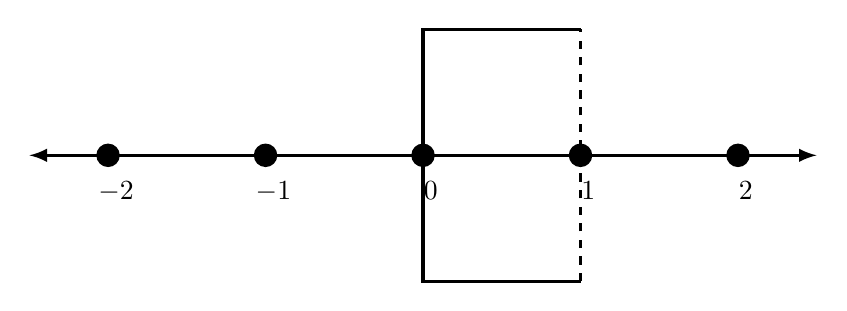
\begin{tikzpicture}[very thick,scale=2]
            \draw[latex-latex] (-2.5,0) -- (2.5,0); 
            \foreach \x in  {-2,-1,0,1,2}
            {
                \node at (\x, 0)[circle,fill,inner sep=3pt]{};
                \draw[shift={(\x+0.05,-0.1)}] node[below] {$\x$};
            }
            \draw[dashed] (1,-0.8) -- (1,0.8);
            \draw (1,0.8) -- (0,0.8) -- (0, -0.8) -- (1, -0.8);
        \end{tikzpicture}}
    \end{center}
    同理可得:
    \[[1]_R = \{y \in \mathbb{R} \mid (1, y) \in \mathbb{R}\} = \{y \in \mathbb{R} \mid 1 \le y < 2\}\]
    如下图所示:

    \begin{center}
        {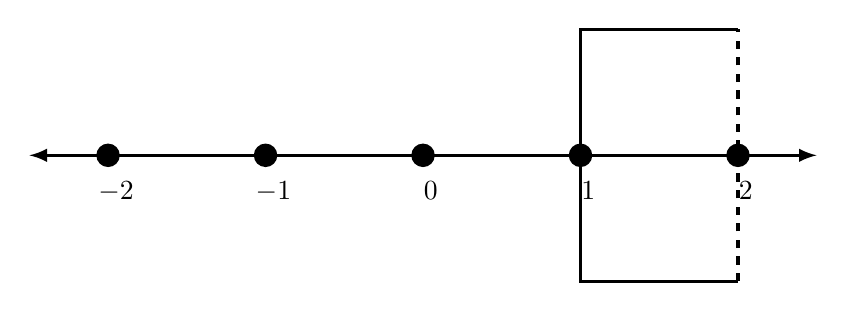
\begin{tikzpicture}[very thick,scale=2]
            \draw[latex-latex] (-2.5,0) -- (2.5,0); 
            \foreach \x in  {-2,-1,0,1,2}
            {
                \node at (\x, 0)[circle,fill,inner sep=3pt]{};
                \draw[shift={(\x+0.05,-0.1)}] node[below] {$\x$};
            }
            \draw[dashed] (2,-0.8) -- (2,0.8);
            \draw (2,0.8) -- (1,0.8) -- (1, -0.8) -- (2, -0.8);
        \end{tikzpicture}}
    \end{center}
\end{example}

注意到 $[0]_R$ 与 $[1]_R$ 互不相交(因为 $1 \notin [0]_R$ 而 $1 \in [1]_R$),且\textbf{每个实数必属于唯一}区间。例如:
\[\pi \in [3]_R, e \in [2]_R, -1.5 \in [-2]_R,\frac{1}{2} \in [0]_R\]
请注意,\emph{等价类}的定义并没有要求我们必须用某个特定元素来\emph{表示}该类。例如,我们也可以说
\[[0]_R = \Big[\frac{1}{2}\Big]_R\]
因为这两个集合是相等的,它们包含相同的元素。任何``向下取整''为 $0$ 的实数在 $R$ 下都与 $0$ 相关,因此在 $R$ 下也与 $\frac{1}{2}$ 相关,因为它们的向下取整都是 $0$。

建议通过此例深入理解划分的性质。后续我们将严格证明该性质的普适性!由于接下来的论证较为抽象,请结合具体实例思考:尝试在其他集合上定义等价关系,观察其等价类,理解其构成划分的必然性。

\subsubsection*{集合的等价类划分}

我们已探讨过等价类对集合的\emph{划分}思想,现在正式定义这个概念。首先给出定义,随后证明一个本质为``当且仅当''的定理。我们将证明其中一个方向,另一方向留作练习。

\begin{definition}
    设 $R$ 为集合 $A$ 上的等价关系,关系 $R$ 下等价类的集合记作 $A / R$,即 $A$ \dotuline{模 (modulo)} $R$。也就是说
    \[A / R = \{[x]_R \mid x \in A\}\]
    换种写法是
    \[A / R = \{X \subseteq A \mid \exists x \in A \centerdot X = [x]_R\}\]
\end{definition}

在证明核心结论前,先通过实例理解概念。每个例子需验证等价关系存在性,检验等价类,并思考模运算的作用。

\begin{example}
    再次考察实数集 $\mathbb{R}$ 上的关系 $R$,其定义为 $(x, y) \in R \iff \lfloor x \rfloor = \lfloor y \rfloor$。此前已说明它是等价关系,现在研究其等价类。

    根据定义,任何两个相关的元素都有相同的等价类。例如,$[0]_R = [0.5]_R = [0.999]_R$。同样地,$[3.5]_R = [3.75]_R, [-\pi]_R = [-4]_R$,但 $[\pi]_R \ne [4]_R$。每个实数 $x \in \mathbb{R}$ 都有一个对应的等价类 $[x]_R$,而模运算的思想是通过只考虑必要的等价类来简化 $R$ 的表示。由于 $[0]_R = [0.5]_R = [0.333]_R$ 等等,我们可以用一个集合 $[0]_R$ 来代表所有这些相同的集合。故有
    \[\mathbb{R} / R = \{\dots, [-2]_R, [-1]_R, [0]_R, [1]_R, [2]_R, \dots \}\]
    实际上,$\mathbb{R} / R$ 可与整数集 $\mathbb{Z}$ 建立对应。然而,我们通常写作 $\mathbb{R} / R ``='' \mathbb{Z}$ 是因为这种等式并不严谨。特别是,我们尚未形式化定义实数或整数,仅仅严格定义了自然数 $\mathbb{N}$。此处仅仅观察到等价类集与整数集存在对应关系,二者可以相互映射,但技术上并非\emph{相等}。

    不过没关系!本例重在说明 $\mathbb{R} / R$ 是等价类的集合。需注意,集合论中元素的顺序和重复无关紧要。如 $\{1, 3, 5, 3, 1\}$ 与 $\{1, 3, 5\}$ 在集合意义上是\emph{同一集合},因为它们含有\emph{相同元素}。同理,$\mathbb{R} / R$ 无需同时包含 $[0]_R$ 和 $[0.5]_R$(二者为同一对象),重复列出无意义。

    通常,我们会关注等价类的表征形式与定性描述,例如:$A/R$ 中类的数量、类的规模(是否等势?是否存在有限类与无限类?)、类元素的描述模式是否一致?

    本例中,$\mathbb{R} / R$ 的所有等价类结构相同。存在可数无限多个等价类(与 $\mathbb{Z}$ 一一对应),每个类均为无穷集且形如实数区间。具体而言,对任意 $z \in \mathbb{Z}$,有 $[z]_R = \{y \in \mathbb{R} \mid z \le y < z + 1\}$。故这些等价类具有\emph{相同结构}。
\end{example}

\begin{example}
    在所有人的集合 $S$ 上定义关系 $B$ 为 $(x, y) \in B \iff x \text{\ 和\ } y \text{\ 同月出生}$。那么 $(\text{欧拉}, \text{庞加莱}) \in B$ 且 $(\text{Paul Erdős}, \text{Emmy Noether}) \in B$。$B$ 是等价关系吗?是的,因为:每个人都与自己的出生月份相同(自反性);若 $x$ 与 $y$ 同月出生,则 $y$ 与 $x$ 必然同月出生(对称性);若 $x$ 与 $y$ 同月出生,且 $y$ 与 $z$ 同月出生,则 $x$ 与 $z$ 同月出生(传递性)。

    (注意:通常由``具有相同……''或``是同一……''定义的关系是等价关系。)

    在此关系下,等价类对应出生月份。每个等价类由同月出生的人组成。例如,Paul Erdős 和 Emmy Noether 均生于三月,故 $\text{Emmy Noether} \in [\text{Paul Erdős}]_B$。该等价类\emph{对应于}三月,但请注意,它是基于集合 $S$(全体人)中的特定元素定义的。

    若定义 $M$ 为所有三月出生者的集合,则 $M = [\text{Paul Erdős}]_B$。综上,按出生月份划分的集合 $S/B$ 包含 $12$ 个子集,每个子集对应一个月份,包含该月出生的所有人。
\end{example}

\begin{example}
    考虑所有有序实数对的集合 $\mathbb{R} \times \mathbb{R}$。在其上定义关系 $R$:
    \[\big((x, y),(u, v)\big) \in R \iff x = u\]
    也就是说,当平面上两点的横坐标相同时,它们在关系 $R$ 下相关。几何上,此关系只关心点所在与 $y$ 轴平行的垂线。由此可以直观理解 $R$ 是等价关系,严格证明只需按定义逐项验证即可。(请尝试证明!)

    该关系下的等价类很容易描述:所有在同一垂线上的点都属于同一个等价类,这些类可用垂线与横轴的交点索引。例如 $(1, 3) \in [(1, 0)]_R$,因为点 $(1, 3)$ 与 $(1, 0)$ 位于同一条垂线上。每个等价类均可表示为 $[(x, 0)]_R$,其中 $x \in \mathbb{R}$。
\end{example}

\begin{center}
    {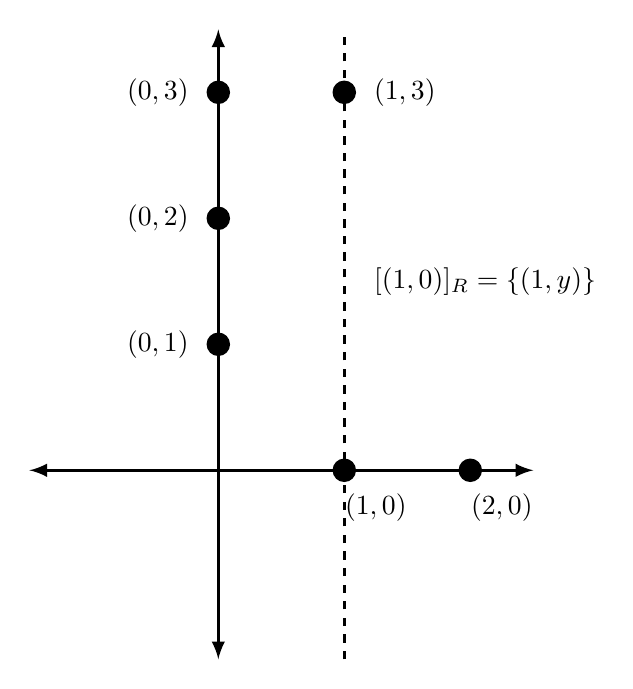
\begin{tikzpicture}[very thick,scale=1.6]
        \draw[latex-latex] (-1.5,0) -- (2.5,0); 
        \draw[latex-latex] (0,-1.5) -- (0,3.5); 
        \foreach \x in  {1,2}
        {
            \node at (\x, 0)[circle,fill,inner sep=3pt]{};
            \draw[shift={(\x+0.25,-0.1)}] node[below] {$(\x, 0)$};
        }
        \foreach \y in  {1,2,3}
        {
            \node at (0, \y)[circle,fill,inner sep=3pt]{};
            \draw[shift={(-0.15, \y)}] node[left] {$(0, \y)$};
        }
        \draw[dashed] (1,-1.5) -- (1,3.5);
        \node at (1, 3)[circle,fill,inner sep=3pt]{};
        \draw[shift={(1.15, 3)}] node[right] {$(1, 3)$};
        \draw[shift={(1.15, 1.5)}] node[right] {$[(1,0)]_R = \{(1, y)\}$};
    \end{tikzpicture}}
\end{center}

因此,在某种意义上,等价类的集合 $(\mathbb{R} \times \mathbb{R})/R$ 与实数轴 $\mathbb{R}$ ``等同''!通过忽略第纵坐标,我们可以将平面上的所有点投影到横轴上。从数学上讲,有一种更精确的方式表达这一观点,但这里不作正式讨论。简而言之,$\mathbb{R} \times \mathbb{R}$ 上的这一关系所生成的等价类对应于 $\mathbb{R}$,这带来了一些有趣的现象。

下面给出 $\mathbb{R} \times \mathbb{R}$ 上的另一个关系。定义 $S$ 为
\[\big((x, y),(u, v)\big) \in S \iff \sqrt{x^2+y^2} = \sqrt{u^2+v^2}\]
回顾基本几何与代数知识,不难发现 $\sqrt{x^2 + y^2}$ 表示点 $(x, y)$ 到原点 $(0, 0)$ 的距离。(在数学中,这类函数被称为\emph{度量 (metric)}。)因此,该关系表明,当两点到原点的距离相等时,它们是等价的。直观上,这解释了 $S$ 是等价关系,且等价类是以原点为中心的圆。于是,我们可以用这些圆的一个显著特征——它们的\emph{半径} $r \ge 0$,来描述集合 $(\mathbb{R} \times \mathbb{R})/S$ 的元素。因此,$S$ 下的等价类集合与非负实数集``等同''!

\begin{center}
    {\begin{tikzpicture}[very thick,scale=2]
        \draw[latex-latex] (-3,0) -- (3,0); 
        \draw[latex-latex] (0,-3) -- (0,3); 
        \foreach \x in  {-2,-1,0,1,2}
        {
            \node at (\x, 0)[circle,fill,inner sep=3pt]{};
            \node at (0, \x)[circle,fill,inner sep=3pt]{};
        }
        \draw[dashed] (0,0) circle (1);
        \draw[dashed] (0,0) circle (2);
        \draw[shift={(0.8, -0.7)}] node[right] {$[(1,0)]_S$};
        \draw[shift={(0.8, -0.9)}] node[right] {$r=1$};
        \draw[shift={(1.7, 1.5)}] node[right] {$[(2,0)]_S$};
        \draw[shift={(1.7, 1.3)}] node[right] {$r=2$};
    \end{tikzpicture}}
\end{center}

这听起来有点奇怪。我们从一个二维集合出发,关联点对并划分出等价类,最终却得到一个一维集合。(注意:我们尚未正式定义\emph{维度 (dimension)},但读者应该能够理解其含义。)回顾上文在 $\mathbb{R}^2$ 上定义的关系 $R$。如果我们将该关系限制在 $\mathbb{R}^2$ 的``右半部分'',即所有横坐标非负的点集上,那么等价类集合也与非负实数集``等同''。在何种意义上,此集合与 $(\mathbb{R} \times \mathbb{R})/S$ ``等同''?这个问题是否合理?我们又该如何\emph{证明}这一结论?这些都是值得思考的有趣问题!

不必过分纠结这些概念与问题。关键在于:等价类的集合构成了原集合的一个\textbf{划分}。

现在我们已经考察了若干例子,接下来我们将陈述(并证明!)等价关系的一些重要结论。核心在于,这些定理印证了我们反复强调的观点:等价关系将集合划分成相应的等价类。然而,有趣的是,我们还有一个逆向结论:给定任意划分,均可定义一个对应的等价关系!

\begin{theorem}\label{theorem6.4.10}
    设 $R$ 为集合 $A$ 上的等价关系。则 $A/R$ 中的集合构成 $A$ 的划分,即这些集合非空、互不相交,且其并集为 $A$。
\end{theorem}

\begin{proof}
    见习题 \ref{exc:exercises6.7.13}
\end{proof}

我们将在本章末尾的习题 \ref{exc:exercises6.7.13} 中引导你完成这一证明。此前讨论的例子有助于你直观理解该定理的正确性,而通过详细的证明推导,你将对其数学严谨性获得扎实的理解。

\subsubsection*{划分产生等价关系}

现在,我们考察一个类似但重要的结论,它实质上是前一个定理的逆命题。为了更好地理解这一定理,我们先分析一个例子,该例子也将提供定理证明的框架。

\begin{example}
    考虑集合 $S=[6]$。定义集合
    \[\mathcal{F} = \big\{ \{1, 4\}, \{2, 3, 5\} , \{6\} \big\}\]
    注意,$\mathcal{F}$ 构成 $S$ 的一个划分,因为这些集合是非空、互不相交,且并集为 $S$。是否存在等价关系 $R$ 使得 $S/R$ 恰好是这些集合?答案是肯定的!尽管难以用类似``$(x, y) \in R \iff x$ 与 $y$ 具有某种共同属性''这种优雅的形式定义,但可以利用划分本身构造关系。具体来说,划分集合就是等价类。划分本身建立了等价类的结构,我们只需通过 $(x, y) \in R \iff x \text{\ 与\ } y \text{\ 属于同一个划分集合}$ 来定义等价关系 $R$。

    本例中,设 $S_1 = \{1, 4\}, S_2 = \{2, 3, 5\}, S_3 = \{6\}$,则 $R$ 可以定义为
    \[(x, y) \in R \iff \exists i \in [3] \centerdot (x \in S_i \land y \in S_i)\]

    请思考为什么这种方法有效。它为何构成等价关系?其等价类是什么?
\end{example}

接下来正式陈述并证明该定理。

\begin{theorem}\label{theorem6.4.12}
    设 $S$ 为集合,$\mathcal{F}$ 为集合 $S$ 的划分。则存在等价关系 $R$ 使得 $S/R=\mathcal{F}$。
\end{theorem}

正如我们之前提到的,此结论的核心在于:划分的子集恰好可视为待定义的等价类。只需证明关系``$x$ 与 $y$ 相关当且仅当$x$ 和 $y$ 属于同一划分子集''是一个等价关系。这并不困难,建议在阅读证明前尝试自行推导!

\begin{proof}
    设 $\mathcal{F}$ 为集合 $S$ 的划分。这意味着存在索引集 $I$ 使得
    \[\mathcal{F} = {S_i \mid i \in I}\]
    其中集合 $S_i$ 满足 $S_i \subseteq S$ 且 $S_i \ne \varnothing$,并且
    \[\bigcup_{i \in I} S_i = S \quad \text{且} \quad \forall i, j \in I \centerdot i \ne j \implies S_i \cap S_j = \varnothing\]
    定义 $S$ 上的关系 $R$ 为
    \[(x, y) \in R \iff \exists i \in I \centerdot (x \in S_i \land y \in S_i)\]
    我们要证明 $R$ 为等价关系。

    \begin{itemize}
        \item \textbf{自反性}:设 $x \in S$ 为任意固定元素。由于 $S_i$ 覆盖 $S$,因此 $\exists i \in I \centerdot x \in S_i$。给定这样的 $i$,则必有 $x \in S_i$ 且 $x \in S_i$,因此 $(x,x) \in R$。故 $R$ 具有自反性。
        
        \item \textbf{对称性}:设 $x, y \in S$ 为任意固定元素。假设 $(x, y) \in R$,这意味着 $\exists i \in I \centerdot (x \in S_i \land y \in S_i)$。给定这样的 $i$,则必有 $y \in S_i \land x \in S_i$,因此 $(y,x) \in R$。故 $R$ 具有对称性。
        
        \item \textbf{传递性}:设 $x, y, z \in S$ 为任意固定元素。假设 $(x, y) \in R$ 且 $(y, z) \in R$,这意味着 $\exists i \in I \centerdot (x \in S_i \land y \in S_i)$ 且 $\exists j \in I \centerdot (y \in S_j \land z \in S_j)$。给定这样的 $i, j$,注意 $y \in S_i \land y \in S_j$,而对于任意不同的 $i,j, S_i \cap S_j = \varnothing$,因此 $i=j$(否则会出现 $y \in \varnothing$,而这是不可能的!)由于 $x \in S_i, y \in S_i, z \in S_i$,因此 $(x,z) \in R$。故 $R$ 具有传递性。
    \end{itemize}
    综上,$R$ 是一个等价关系!

    $S/R$ 的等价类写做 $[x]_R$,其中 $x \in S$。因为 $\mathcal{F}$ 是 $A$ 的划分,对于任意 $x \in S$,存在 $i$ 使得 $x \in S_i$。因此所有等价类均属于 $\mathcal{F}$。

    类似地,对于任意非空集合 $S_i \ne \varnothing$,都有 $\exists x \in S_i$,因此存在对应的等价类 $S_i=[x]_R$。故每个等价类都是形如 $S_i$ 的集合,反之亦然。
\end{proof}

这表明,任意划分都唯一对应一个等价关系及其等价类!


% !TeX root = ../../../book.tex

\subsection{更多示例}

现在我们已经掌握了这两个定理,让我们通过一些关系的例子来进一步理解它们。对于每个例子,我们将尝试判断它是否是等价关系。如果是,我们可以描述它的等价类。如果不是,我们可以参考其中一个定理,看看为什么它不是等价关系。\\

\begin{example}
    我们先从一个简单的例子开始。回顾一下我们在示例 \ref{ex:example6.2.9} 中定义的等式关系。我们已经解释过,``$=$'' 在任何集合上都是等价关系。具体来说,它将一个集合划分为等价类,而这些等价类正是集合的各个元素本身。例如,在集合 $\mathbb{N}$ 中,$[1]_{=} = \{1\}, [2]_{=} = \{2\}$,依此类推。所有的等价类都是\emph{单例的}(集合只有一个元素)。
\end{example}

\begin{example}
    我们再来看一个相对简单的例子。回顾一下我们在示例 \ref{ex:example6.2.5} 中定义的 $\mathbb{Z}$ 集合上的奇偶关系。这是一个等价关系,现在让我们来证明这一点。
    \begin{proof}
        设 $a, b, c \in \mathbb{Z}$ 是任意的。

        首先,不难发现 $(a,a) \in R$ 因为 $a$ 与其自身有相同的奇偶性。因此 $R$ 具有自反性。

        其次,假设 $(a,b) \in R$,所以 $a$ 和 $b$ 具有相同的奇偶性。那么显然 $b$ 和 $a$ 也具有相同的奇偶性,所以 $(b,a) \in R$。因此 $R$ 具有对称性。

        最后,假设 $(a,b) \in R$ 且 $(b,c) \in R$。如果 $a$ 是奇数,我们可以推导出 $b$ 为奇数且 $c$ 也为奇数;同理,如果 $a$ 为偶数,我们可以推导出 $b$ 为偶数且 $c$ 也为偶数。无论是哪种情况,$a$ 和 $c$ 都具有相同的奇偶性,所以必然有 $(a,c) \in R$。因此 $R$ 具有传递性。

        因为 $R$ 具有自反性、对称性和传递性,所以 $R$ 是一个等价关系。
    \end{proof}

    这意味着等价类集合 $\mathbb{Z}/R$ 构成 $\mathbb{Z}$ 的划分。现在让我们来确定该划分。

    考虑 $[0]_R$,这是所有与 $0$ 奇偶性相同的整数集合,即所有\emph{偶数}。因此,在这种情况下,
    \[\mathbb{Z}/R = \{O_{\mathbb{Z}}, E_{\mathbb{Z}}\}\]
    其中 $O_{\mathbb{Z}}$ 是奇数集,$E_{\mathbb{Z}}$ 是偶数集。这两个等价类都是无穷大的。
\end{example}

\begin{example}
    回顾我们在示例 \ref{ex:example6.2.6} 中定义的 $\mathbb{R}$ 上的顺序关系。这个关系是等价关系吗?我们可以通过检查定义中的每个属性来确定。要注意的是,无论 $x$ 是什么,只要 $x \in \mathbb{R}$,就有 $(x, x) \notin R$,因为 $x \nless x$。因此,$R$ 不具有自反性,所以它不是等价关系。(另外,$R$ 也不具有对称性,但它具有传递性。)

    为什么严格的顺序关系不会是等价关系呢?为什么我们希望等价关系是自反的?想想\emph{等价类}的概念;等价关系应该把整个集合的元素划分成几部分,我们可以通过属于某部分的一个元素来识别这部分。对于非自反的关系,有些元素不属于它们自己的``等价类'',这显然是不理想的!

    (后续问题:对于自反的顺序关系 $\le$,它是等价关系吗?为什么是或者为什么不是?)
    
    换句话说,$\mathbb{R}$ 上的 ``$<$'' 关系并没有把实数划分为几部分。基于这一点,并结合定理 \ref{theorem6.4.10} 的\emph{逆否}命题,我们可以得出 ``$<$'' \emph{不是}一个等价关系。
\end{example}

\begin{example}
    定义 $\mathbb{R} \times \mathbb{R}$ 上的关系 $\sim$ 为
    \[(x, y) \sim (u, v) \iff x \le u \land y \le v\]
    即使不检查其具体属性,我们也可以尝试判断它是否是等价关系。为此,我们选取集合中的一个特定元素,并查看与该特定元素相关的所有元素。在下图中,我们使用 $(1, 1)$ 作为这个特定元素。

    \begin{center}
        {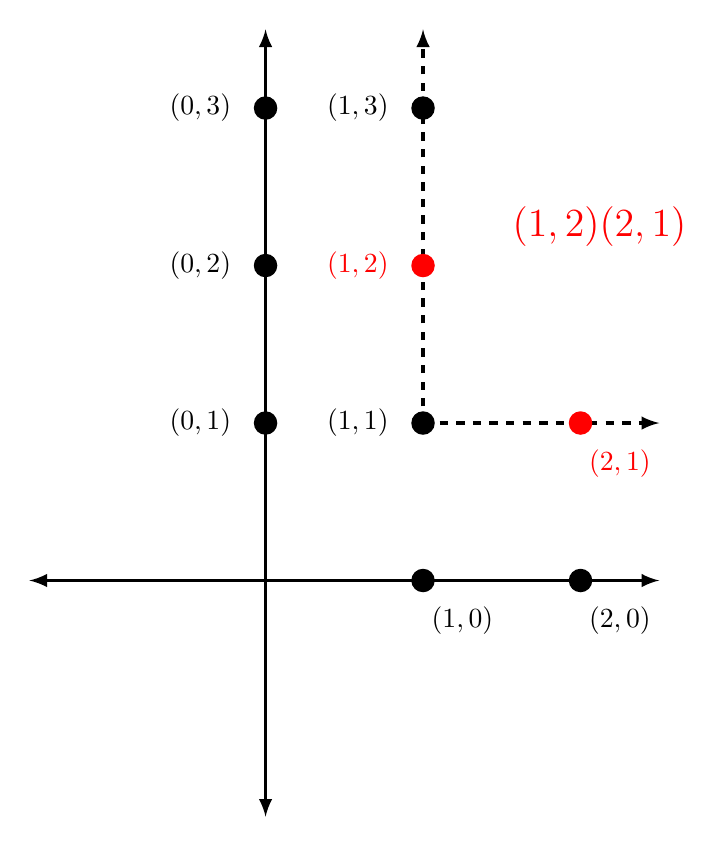
\begin{tikzpicture}[very thick,scale=2]
            \draw[latex-latex] (-1.5,0) -- (2.5,0); 
            \draw[latex-latex] (0,-1.5) -- (0,3.5); 
            \foreach \x in  {1,2}
            {
                \node at (\x, 0)[circle,fill,inner sep=3pt]{};
                \draw[shift={(\x+0.25,-0.1)}] node[below] {$(\x, 0)$};
                
            }
            \foreach \y in  {1,2,3}
            {
                \node at (0, \y)[circle,fill,inner sep=3pt]{};
                \draw[shift={(-0.15, \y)}] node[left] {$(0, \y)$};
            }
    
            \draw[dashed,-latex] (1,1) -- (2.5,1); 
            \draw[dashed,-latex] (1,1) -- (1,3.5); 
            \foreach \y in  {1,3}
            {
                \node at (1, \y)[circle,fill,inner sep=3pt]{};
                \draw[shift={(0.85, \y)}] node[left] {$(1, \y)$};
            }
    
            \node[red] at (1, 2)[circle,fill,inner sep=3pt]{};
            \draw[color=red, shift={(0.85, 2)}] node[left] {$(1, 2)$};
            \node[red] at (2, 1)[circle,fill,inner sep=3pt]{};
            \draw[color=red, shift={(2.25, 0.9)}] node[below] {$(2, 1)$};
    
            \draw[color=red, font=\Large, shift={(1.5, 2.25)}] node[right] {$(1,2) \nsim (2,1)$};
        \end{tikzpicture}}
    \end{center}

    请注意,$\sim$ 的定义条件要求一个点必须位于另一个点的``右上方''才能使两者相关。同时,不等式是``$\le$'',因此第二个点不必\emph{严格}位于上方或右侧。

    因此,我们可以从上图看到,$(1, 2) \sim (1, 1)$(因为 $1 \le 1$ 且 $1 \le 2$)。同理,$(1, 1) \sim (2, 1)$。因此,点 $(1, 2)$ 和 $(2, 1)$ 都与 $(1, 1)$ 相关。为了使 $\sim$ 成为\emph{等价关系},我们需要 $(2, 1$) 和 $(1, 2)$ 也彼此相关。因为它们必须同属于 $(1, 1)$ 的``等价类''。然而,遗憾的是,$(1, 2) \nsim (2, 1)$。第二个点严格位于第一个点的``左下方'',因此不满足 $\sim$ 的定义条件。

    这意味着所有与 $(1, 1)$ 相关的元素的集合\textbf{不能}形成一个``封闭集合''。从数学上讲,这些元素的集合不是一个等价类。因此,$\sim$ \textbf{不是}一个等价关系。

    现在,试着识别 $\sim$ 具有哪些性质和不具备哪些性质。它具有自反性吗?具有对称性吗?具有传递性吗?为什么具有或者为什么不具有?通过这样做,你会再次证明 $\sim$ 不是一个等价关系。事先弄清楚这一点,是不是很有帮助呢?我们建议,当你遇到一个定义好的关系时,可以做类似的分析。你能找出``等价类''可能是什么吗?如果能,那么你对这个关系为何以及如何是等价关系有了一些直觉,这将帮助你描述等价类。如果不能,那么你也会对如何反驳这种说法有一些理解。
\end{example}

\subsubsection*{[选学] $\mathbb{Z}$ 是如何从 $\mathbb{N} \times \mathbb{N}$ 上的等价关系生成的}

还记得第 \ref{ch:chapter03} 章中的那个复杂习题吗?它要求你证明某些关于自然数对的性质,并声称这是在证明整数的存在性。那到底是怎么回事呢?现在回头看看习题 \ref{exc:exercises3.11.22}。你会发现问题的最后三个部分要求你证明我们定义的集合 $R$ 是集合 $P$ 上的\textbf{等价关系}(底层集合是 $P = \mathbb{N} \times \mathbb{N}$)。好好看一下!你已经证明了 $R$ 具有自反性、对称性和传递性。

这个练习表明(在这里我们略过了一些细节)任何负整数都可以表示为两个整数之差为该负整数的\textbf{等价类}。也就是说
\[-1 \;\text{``$=$''}\; [(1, 2)]_R = \{(1, 2),(2, 3),(3, 4), \dots \}\]
再比如
\[-3 \;\text{``$=$''}\; [(1, 4)]_R = \{(1, 4),(2, 5),(3, 6), \dots \}\]
这只是一个直观的解释,从数学上讲并不严格,但这就是主要思路!


% !TeX root = ../../../book.tex

\subsection{习题}

\subsubsection*{温故知新}

以口头或书面的形式简要回答以下问题。这些问题全都基于你刚刚阅读的内容,如果忘记了具体定义、概念或示例,可以回顾相关内容。确保在继续学习之前能够自信地作答这些问题,这将有助于你的理解和记忆!

\begin{enumerate}[label=(\arabic*)]
    \item \emph{等价关系}需要满足哪些性质?
    \item 什么是等价类?等价类中的所有元素必须满足什么条件?
    \item 给定集合 $S$ 和 $S$ 上的等价关系 $R$,等价类的集合必须满足什么条件?
\end{enumerate}

\subsubsection*{小试牛刀}

尝试解答以下问题。这些题目需动笔书写或口头阐述答案,旨在帮助你熟练运用新概念、定义及符号。题目难度适中,确保掌握它们将大有裨益!

\begin{enumerate}[label=(\arabic*)]
    \item 回顾 \ref{sec:section6.2.5} 节习题 \ref{exc:exercises6.2.2} 中定义的关系。我们在该习题中定义 $\mathbb{Z}$ 上的关系 $\bigstar$ 为
    \[\forall x, y \in \mathbb{Z} \centerdot x \;\bigstar\; y \iff 3 \mid x - y\]
    之前已经证明了它确实是一个等价关系。现在,请描述 $\mathbb{Z}/\bigstar$ 的等价类。有多少个等价类?每个等价类的大小如何?能否列出其元素或描述其特征?
    \item 回顾 \ref{sec:section6.2.5} 节习题 \ref{exc:exercises6.2.3} 中定义的关系。我们在该习题中定义 $\mathbb{Z}$ 上的关系 $\sim$ 为
    \[\forall x, y \in \mathbb{Z} \centerdot x \sim y \iff 3 \mid x + 2y\]
    之前已经证明了它确实是一个等价关系。现在,请判别并描述 $\mathbb{Z}/\sim$ 的等价类。有多少个等价类?的大小如何?能否列出其元素或描述其特征?对比上一题,你有什么发现?
    \item 考虑集合 $[5]=\{1,2,3,4,5\}$。定义 $[5]$ 上的关系 $\approx$ 为,对于任意 $x,y \in [5]$
    \[x \approx y \iff \vert x^2 - y^2 \vert \le 5\]
    对于任意 $x \in [5]$,设 $S(x)$ 为满足 $x \approx y$ 且 $y \in [5]$ 的所有元素的集合。
    \begin{enumerate}[label=(\alph*)]
        \item 列出集合 $S(1), S(2), S(3), S(4), S(5)$ 中的所有元素。
        \item 通过观察这些集合,能否判断 $\approx$ 是否是一个等价关系?依据是什么?
        \item 通过证明或证伪自反性、对称性和传递性,来验证 $\approx$ 是否是一个等价关系。
    \end{enumerate}
    \item 考虑集合 $\mathbb{N} \times \mathbb{N}$。定义该集合上的关系 $\sim$ 为
    \[(a, b) \sim (c, d) \iff a + b = c + d\]
    判断该关系否是一个等价关系。如果是,请可视化地描述其等价类。
\end{enumerate}

\newpage
% !TeX root = ../../../book.tex
\section{模算术}

你可能已经接触过一种自然而常见的等价关系,即整数上的\emph{同余}关系。这是对``奇偶性''等价关系的直接推广,它基于某个特定属性对整数进行分类。在此,我们将通过定义整数的某些性质来扩展这一概念,并引入多个等价类。我们还将探讨一些有趣的结论,这些结论利用同余关系使问题的证明变得更加简便(甚至成为可能!)。

% !TeX root = ../../../book.tex

\subsection{定义与示例}

\subsubsection*{整除性}

我们从熟悉的基本定义开始。

\begin{definition}
    设 $a,b \in \mathbb{Z}$。若存在整数 $k \in \mathbb{Z}$ 使得 $b = ak$(等价地,当 $a \neq 0$ 时 $\frac{b}{a} \in \mathbb{Z}$),则称 $a$ \dotuline{整除} $b$(或 $b$ 可以被 $a$ 整除)。记作 $a \mid b$。
\end{definition}

注意,根据定义,任意非零整数均可整除 $0$(例如 $5 \mid 0$),但 $0$ 仅能整除自身(例如 $0 \nmid 5$ 但 $0 \mid 0$)。请思考这与``整除''的直观理解是否一致。定义中 $k \in \mathbb{Z}$ 的约束允许负数参与运算,因此 $-2 \mid 4$ 和 $8 \mid -24$ 均成立。

诸如 $2 \nmid 5$ 这样的表述揭示了整数间的关系,但并未涵盖所有情况。虽然没有整数 $k$ 满足 $2k=5$,但 $k=2$ 和 $k=3$ 分别给出 $4$ 和 $6$,都非常接近 $5$;而 $k = -100$ 则偏差很远。对于较小数字通常易于验证,但当数字较大时,例如 $7 \nmid 100000$(由质数性质可知),如何找到使 $7k$ 最接近 $100000$ 的 $k$ 呢?答案是否唯一?是否存在多个``合理''选项(如 $2 \nmid 5$ 的情形)?

关于上面第二个问题,为了简化问题,我们需要限定答案,使其只有唯一合理选项。这样才能避免在得到一个答案后还要担心是否还有其他答案。为此,我们将借鉴\emph{价格猜猜猜 (The Price Is Right)}\footnote{《价格猜猜猜》是美国历史上播出时间最长的一档电视节目。—— 译者注}的规则:寻找\emph{最接近但不超过}目标值的答案。比如在 $2 \nmid 5$ 的例子中,我们认为 $k = 2$ 是最佳估计,因为 $4 < 5$。同理,在 $7 \nmid 100000$ 的例子中,我们认为 $k = 14285$ 是最佳估计,因为 $7 \times 14285 = 99995 < 100000$。(注意,在这种情况下,有一个``更接近''的估计,但它超过了目标值,因此我们不予考虑。)

这就引出了另一个问题——如何获得此类估计?对给定 $a,b \in \mathbb{Z}$,可以递增计算 $a$ 的倍数直至超过 $b$,其前一个倍数即为最优解。估计的``准确性''范围在 $0$ 到 $a - 1$ 之间,当 $a$ 能整除 $b$ 时,准确性为 $0$。(注意:``超过''是指顺序关系 $>$,因此负数情形需谨慎处理次序关系。如 $2 \nmid -3$ 时取 $k=-2$,因为 $-4 \le -3$。)下述引理总结了递增计算 $a$ 的倍数直到找到 $b$ 的最佳估计的思路,并阐明在限定条件下,总存在唯一解。

\begin{lemma}[除法算法]\label{lemma6.5.2}
    设 $a,b \in \mathbb{Z}$。$\exists k, r \in \mathbb{Z}$ 使得 $ak + r = b$,其中 $0 \le r \le a - 1$。换句话说,对于任意两个整数,总能找到一个 $a$ 的倍数 $k$,使得 $k$ 与 $a$ 的乘积最接近但不超过 $b$,同时还会得到唯一一个余数 $r$。我们把 $r$ 称为``$b$ 除以 $a$ 的余数''或``$b$ 被 $a$ 除的余数''。
\end{lemma}

余数概念至关重要,我们会频繁使用。后续将基于余数比较定义等价关系。首先请证明此引理!

\begin{proof}
    留作习题 \ref{exc:exercises6.7.14}。
\end{proof}

之所以称之为除法\emph{算法},是因为它提供了一种\emph{求解}倍数和余数的\emph{机制}。这种方法虽然简单但非常有效,简而言之就是\emph{反复应用减法}。也就是说,给定 $a$ 和 $b$,不断地从 $b$ 中减去 $a$,例如先得到 $b - a$,再得到 $b - 2a$,然后是 $b - 3a$……依此类推,直到剩下一个介于 $0$ 到 $a$ 之间的余数。

\begin{example}
    让我们通过一个例子来展示这一过程。假设 $a = 8, b = 62$。我们不断地从 $62$ 中减去 $8$,结果是:
    \[62, 54, 46, 38, 30, 22, 14, 6\]
    最终在 $6$ 上停止,因为它满足 $0 \le 6 < a = 8$,这表明余数 $r = 6$。我们还注意到,我们总共从 $b$ 中减去了 $7$ 次 $a$,因为列表中有 $8$ 项,其中第一项是 $b - 0 \cdot a$。故有:
    \[\underbrace{62}_{b} = \underbrace{7}_{k} \cdot \underbrace{8}_{a} + \underbrace{6}_{r}\]
\end{example}

此过程表明余数存在且唯一。利用该结果,可定义 $\mathbb{Z}$ 上的特定关系。下文将证这些关系均为等价关系,并探讨其等价类的强大应用!

这里的重点是有一种方法可以找到余数,并且余数唯一。利用该结果,我们可以定义 $\mathbb{Z}$ 上的特定关系。下文将证明这些关系均为等价关系,并探讨其\emph{等价类}的强大应用!

\subsubsection*{模 $n$ 同余}

\begin{definition}\label{def:definition6.5.4}
    设 $n \in \mathbb{N}$。定义 $\mathbb{Z}$ 上的关系 $R_n$ 为 $(a,b) \in R_n$ 当且仅当 $a$ 和 $b$ 除以 $n$ 的余数相同,即
    \[(a,b) \in R_n \iff n \mid a-b\] 
    亦可记作
    \[a \equiv b \mod n\]
    读作``$a$ 与 $b$ \dotuline{模 $n$ 同余}''。(口头上通常将 ``modulo'' 简化为 ``mod''。)
\end{definition}

\begin{remark}
    定义中``$a$ 和 $b$ 除以 $n$ 的余数相同''等价于 $n \mid a - b$。此结论需要证明,稍后将在习题 \ref{exc:exercises6.7.15} 中完成论证。
\end{remark}

\begin{remark}
    实际应用(如解题与证明)中,$a \equiv b \mod{n}$ 表明可将 $a$ 表示为 $n$ 的倍数与 $b$ 之和。
\end{remark}

我们来看一下为什么这是成立的。假设二者的余数均为 $r$,这意味着存在 $k, \ell \in \mathbb{Z}$ 使得
\[a = kn + r \quad\text{且}\quad b = \ell n + r\]
(余数相同,但 $n$ 的倍数可能不同。)通过相减消去 $r$ 即可得到等式
\[a - kn = b - \ell n\]
然后移项并提取公因式可得
\[a = (k - \ell)n + b\]
此处 $(k - \ell)n$ 是 $n$ 的倍数,而第二项只包含 $b$ 本身。这说明 $a$ 是 $n$ 的倍数加上 $b$。

通常情况下,$b$ 可能并不是 $a$ 除以 $n$ 后的余数;特别是当 $b$ 不满足余数要求 $0 \le r \le a - 1$ 时,就会出现这种情况。

让我们总结一下此观点,并给出后续证明与示例中常用的\emph{模 $n$ 同余}的等价表述:

\setlength{\fboxrule}{2pt}
\begin{center}
\fcolorbox{olivegreen}{white}{%
    \parbox{0.8\textwidth}{%
        \[a \equiv b \mod n \iff \exists m \in \mathbb{Z} \centerdot a=mn+b\]
    }
}
\end{center}

\begin{example}
    让我们通过考察几个较小的 $n$ 值,来考察这些关系的具体表现。

    \begin{itemize}
        \item 设 $n=1$。关系 $R_1$ 会是什么样?这个问题实际上有些无聊,因为任何整数除以 $1$ 的余数都是 $0$,所以每个整数都可以和其他任意整数相关联。也就是说,$\forall x,y \in \mathbb{Z} \centerdot (x, y) \in R_1$。由于这个关系相对平凡,因此数学家们几乎不会讨论``模 $1$''这个话题。
        
        \item 设 $n=2$。关系 $R_2$ 就是我们之前定义的``奇偶关系''。想想为什么会这样。当我们把任意整数 $a$ 除以 $2$ 时,余数只能是 $0$ 或 $1$。如果 $a$ 和 $b$ 除以 $2$ 的余数都是 $0$,那么它们都是偶数;如果余数都是 $1$,那么它们都是奇数。(回想一下我们在第 \ref{ch:chapter03} 章中的定义,\emph{奇数}和\emph{偶数}是通过\emph{存在}声明来定义的。例如,当且仅当 $\exists k \in \mathbb{Z}$ 使得 $x = 2k$ 时,$x$ 为偶数。这正是除法算法的结果。当且仅当 $x$ 除以 $2$ 的余数为 $0$ 时,$x$ 为偶数,因为我们可以找到一个整数 $k$,使得 $x = 2k$。)\\
        现在,想想同余的另一种表述。如果两个整数都是偶数,那么它们的差也是偶数!也就是说,$a \equiv b \mod 2 \iff a - b \mid 2$;即 $a$ 和 $b$ 都是偶数(或者都是奇数)当且仅当它们的差也是偶数。(注意:我们还没有\emph{证明}这种表述确实等价于余数的定义。我们将在本例之后给出证明。)

        \item 设 $n=3$。例如,$0 \equiv 9 \mod 3, -1 \equiv 2 \mod 3$ 以及 $4 \equiv 28 \mod 3$。一般来说,只要在行尾加上``$\text{mod\ } 3$''(或其他数字),便可以连接多个同余语句。如此连接后,整行都按照模 $3$ 处理。例如,以下语句在符号上是有效的,在数学上也是成立的:
        \[-100 \equiv -1 \equiv 8 \equiv 311 \equiv -289 \equiv 41 \mod 3\]
        (虽然我们不确定为什么需要写出这样的陈述,但这样做是完全可以的!)

        \item 设 $n=10$。自然数除以 $10$ 的余数就是它的最后一位数字,即个位数字!这样我们就可以轻松地比较两个数模 $10$ 的余数。例如,$12 \equiv 32 \equiv 448237402 \mod 10$;而 $37457 \not\equiv 38201 \mod 10$。\\
        但对于\emph{负数}的情况会略有不同。因为我们定义余数时,是取\emph{不超过}目标值的最大倍数。例如,$-1 \equiv 9 \mod 10$,这是因为 $-1= (-1) \cdot 10 + 9$,而 $9 = (0) \cdot 10 + 9$。它们的余数都是 $9$,需要加到某个 $10$ 的倍数上。请思考以下陈述的具体细节:
        \[-3 \equiv 17 \equiv -33 \equiv 107 \mod 10\]
    \end{itemize}
\end{example}

\subsubsection*{符号}

需要强调的是,在数学中,\textbf{mod} 是一种关系,而非运算符或函数。在计算机科学和编程中,你可能会看到类似``\verb|5 mod 3 = 2|''这样的表达,它表示``$5$ 除以 $3$ 的余数是 $2$''。(在许多编程语言中,写作 \verb|5 % 3 = 2|)。但数学中不采用这种写法:我们使用 $\text{mod}$ 和 $\equiv$ 符号表示一种\textbf{等价关系},因为讨论的数字不一定\emph{相等}。当等价关系在某个自然数 $n$ 下成立时,我们在行末标注``$\text{mod\ } n$''以指明这一点。此时,$\text{mod}$ 相当于一个\emph{修饰符},表示``本行所有陈述仅对模 $n$ 的余数成立''。例如:
\[100 \equiv 97 \equiv 16 \equiv 4 \equiv z \cdot w \equiv 1 \equiv x - y \equiv -2 \equiv -8 \mod 3\]
这表示在 $\mod 3$ 下,所有数字和表达式等价。我们既不断言它们绝对相等,也不断言其在其他模数下等价;行末的``$\mod 3$''表示``仅在整数模 $3$ 的范围内讨论''。

(问题:你能找到 $x, y, z, w \in \mathbb{Z}$ 使上述等式成立吗?)

\subsubsection*{三个重要引理}

本节要求你证明两个关键结论:第一,模 $n$ 同余可以用\emph{可除性}等价定义;第二,该关系是等价关系。阅读时请完成对应的练习。掌握这些细节后,下一节关于等价类的内容会更容易理解。完成证明后,我们将展示并证明另一引理,并在讨论等价类之前给出一个同余的典型应用:它能简化手工计算繁琐的算术问题。

\begin{lemma}\label{lemma6.5.8}
    在定义 \ref{def:definition6.5.4} 中,模 $n$ 同余的两种表述等价。即对于所有 $a, b \in \mathbb{Z}$ 和 $n \in \mathbb{N}$,
    \[a, b \text{\ 除以\ } n \text{\ 余数相同\ } \iff n \mid a - b\]
\end{lemma}

\begin{proof}
    见习题 \ref{exc:exercises6.7.15}
\end{proof}

\begin{lemma}\label{lemma6.5.9}
    对于任意 $n \in \mathbb{N}, R_n$ 是 $\mathbb{Z}$ 上的等价关系。
\end{lemma}

\begin{proof}
    见习题 \ref{exc:exercises6.7.16}
\end{proof}

感谢你证明了这些引理!$\smiley{}$ 现在我们知道模 $n$ 同余是等价关系(因此可以讨论等价类),且判断两个整数(如 $a$ 和 $b$)模 $n$ 同余等价于验证 $a - b$ 是否是 $n$ 的\emph{倍数},这是一种高效的判定方法。

下一引理表明:``模 $n$''意义下的加法和乘法\textbf{保持同余性}。若有两个整数等式,如 $a + b = c$ 和 $d + e = f$,相加可得 $a + b + d + e = c + f$。此引理说明该原理对模 $n$ 同余同样成立——同余式可相加或相乘,同余关系仍然成立。

尽管该引理的证明并不复杂,但我们将替你完成,因为本节你已经做了太多工作了。

\begin{lemma}[模算术引理 (Modular Arithmetic Lemma, 简称 MAL)]\label{lemma6.5.10}
    设 $n \in \mathbb{N}$。设 $a,b,r,s \in \mathbb{Z}$ 为任意固定整数。若 $a \equiv r \mod n$ 且 $b \equiv s \mod n$,则
    \begin{align*}
        a + b &\equiv r + s \mod n \\
        a \cdot b &\equiv r \cdot s \mod n
    \end{align*}
\end{lemma}

(该引理表明只需处理余数:无论给定的 $a$ 和 $b$ 是什么,均可简化为余数 $r$ 和 $s$ 后进行运算。由于 $0 \le r, s \le n - 1$,其值比 $a$ 和 $b$ 更小,因此可以加速实际运算。以下证明确保该方法普遍成立。)

\begin{proof}
    假设 $a \equiv r \mod n$ 且 $b \equiv s \mod n$。这意味着 $\exists k, \ell \in \mathbb{Z}$ 使得
    \begin{align*}
        a &= kn + r \\
        b &= \ell n + s
    \end{align*}
    \begin{itemize}
        \item 两式相加得
            \[a + b = (kn + r) + (\ell n + s) = (k + \ell)n + (r + s)\]
            因为可以将 $a+b$ 表示为 $n$ 的倍数加上余数 $r+s$,所以 $a + b \equiv r + s \mod n$。
        \item 两式相乘得
            \[a \cdot b =  (kn + r) \cdot (\ell n + s) = k\ell n^2 + (ks + \ell r)n + r \cdot s = n \cdot (k\ell n + ks + \ell r)+r \cdot s\]
            因为可以将 $a \cdot b$ 表示为 $n$ 的倍数加上余数 $r \cdot s$,所以 $a \cdot b \equiv r \cdot s \mod n$。
    \end{itemize}
\end{proof}

\begin{remark}
    请注意,此处仅讨论加法和乘法,未涉及\textbf{减法}和\textbf{除法},原因有二:

    其一,减法本质是``加负数''。该引理表明,对同余作减法可通过两步实现:
    \begin{enumerate}[label=(\arabic*)]
        \item 将其中一个同余乘以 $-1$(应用\emph{乘法}引理)
        \item 将结果相加(应用\emph{加法}引理)
    \end{enumerate}
    此过程巧妙地结合了两个引理的结果。

    其二较为复杂。实际上,模 $n$ 运算中无``除法''运算。主要原因在于讨论范围仅限于\emph{整数},而除法可能产生非整数的\emph{有理数}。例如 $4 \equiv 7 \mod 3$,但 $\frac{4}{2} \equiv \frac{7}{2} \mod 3$ 无意义——整数(如 $2$)不能与非整数(如 $\frac{7}{2}$)同余。因此在 $\mathbb{Z}$ 模 $n$ 系统中不定义\textbf{除法}。

    ``除法''问题存在更精细的讨论,将在 \ref{sec:section6.5.3} 节讨论\emph{乘法逆元}时详述。为了避免混淆,此处暂不展开。简而言之,后续将发展一种在特定条件下类似模 $n$ 除法的方法。

    综上,为了保持\emph{整数}范畴,本书仅讨论加法与乘法。
\end{remark}

\subsubsection*{两个实用例子}

我们可能尚未完全说服你认识到模算术的妙用。为了展示同余作为等价关系兼具数学趣味与实用价值,这里将展示两个典型示例。第一个例子中,模算术提供了比常规方法更简洁的解法;第二个则是你可能用过却未曾深究的巧妙技巧——我们将证明其有效性。

\begin{example}
    思考以下问题:

    是否\emph{存在}自然数 $k$,使得 $5^k$ 恰好比 $7$ 的倍数多 $1$?如果存在,这样的自然数最小是多少?能否描述所有满足条件的自然数?

    我们可以尝试代入不同的 $k$ 值来寻找答案,但很快会发现:大指数的计算十分繁琐,而验证一个大数是否满足条件更为困难。如果你愿意的话可以自行尝试,甚至借助计算器探索解法。

    不过,我们更倾向反复使用模算术引理 (Modular Arithmetic Lemma, MAL)。由于指数的本质是重复乘法,可以反复运用乘法引理。核心思路是:在连续乘以 $5$ 的过程中,始终保持对 $7$ 取模。我们只需寻找模 $7$ 余 $1$ 的数,无需直接计算其具体值。过程如下:

    从 $5^1 \equiv 5 \mod 7$ 开始。将其乘以 $5$ 得
    \[5^2 \equiv 5 \cdot 5 \equiv 25 \equiv 4 \mod 7\]
    注意到 $25 = 21 + 4$,并且已知 $21$ 是 $7$ 的倍数,从而得出上述结论。(当数字较小时,我们常常可以通过简单观察直接心算。当然,如果不确定,也可以使用除法算法,从 $25$ 中不断减去 $7$,直到剩下余数。)

    继续乘以 $5$ 得
    \[5^3 \equiv 5^2 \cdot 5 \equiv 4 \cdot 5 \equiv 20 \equiv 6 \mod 7\]
    我们发现,通过``观察''可知 $20 = 14+6$。请注意,求 $5^3$ 模 $7$ 的余数并不需要实际计算 $5^3 = 125$ 然后再取模。因为我们在此过程中已经将所有数字都化简到模 $7$ 的余数,所以省去了大量计算。具体来说,我们总是将数字化简到\emph{小于} $7$ 的范围内,因此在任何情况下我们需要处理的最大数字也只会在 $20$ 到 $30$ 之间。这真是太方便了!让我们继续看接下来会得到什么结果:
    \begin{align*}
        5^4 &\equiv 5^3 \cdot 5 \equiv 6 \cdot 5 \equiv 30 \equiv 2 \mod 7 \\ 
        5^5 &\equiv 5^4 \cdot 5 \equiv 2 \cdot 5 \equiv 10 \equiv 3 \mod 7 \\
        5^6 &\equiv 5^5 \cdot 5 \equiv 3 \cdot 5 \equiv 15 \equiv 1 \mod 7 
    \end{align*}
    这正是我们要找的结果!我们已经确定 $5^6$ 比 $7$ 的倍数多 $1$。这种方法比直接计算 $5^6 = 15625$ 并找出 $15625 = 7 \cdot 2232 + 1$ 要简单得多。

    至此解答了前两问:存在满足条件的 $5$ 的幂,且由 $k=1$ 逐步推导可知 $k=6$ 为最小值。第三问留作思考:请继续乘以 $5$ 并观察余数规律。你能否发现模式?提出猜想并尝试证明!(后续将回归此例……)
\end{example}

\begin{example}\label{ex:example6.5.13}
    考虑数字 $474$。它是 $3$ 的倍数吗?只需将各位数字相加:$4 + 7 + 4 = 15$。由于 $15$ 是 $3$ 的倍数,可知 $474$ 也必然是 $3$ 的倍数。(当然,也可通过长除法验证 $474 = 3 \cdot 158$。)但为什么这种方法成立?难道仅仅是因为老师曾在三年级时告诉了你这个方法,你就记住了?这对我们来说远远不够!$\smiley{}$

    这里,我们将严格\textbf{证明}:自然数 $x$ 能被 $3$ 整除当且仅当其各位数字之和能被 $3$ 整除。(证明中括号内的例子仅用于辅助理解。需要注意的是,具体实例不能替代普遍结论的证明。)

    \begin{proof}
        设 $x \in \mathbb{N}$ 为任意固定自然数。其十进制展开形式为
        \[x= \sum_{k=0}^{n-1} x_k \cdot 10^k\]
        其中 $n$ 为数字 $x$ 的位数,$x_k$ 为 $10^k$ 位对应的数字,所以 $0 \le x_k \le 9$。(即 $x_k$ 是从右向左第 $(k+1)$ 位数字。)

        (例如,$47205$ 可写做 $47205=4 \cdot 10^4+7 \cdot 10^3+2 \cdot 10^2+0 \cdot 10^1+5 \cdot 10^0$。本例中,$x_0 = 5, x_1=0, x_3=2$。)

        该整除技巧声称
        \[x \equiv 0 \mod 3 \iff \sum_{k=1}^{n-1} x_k \equiv 0 \mod 3\]

        为了证明这一点,我们将考虑十进制展开模 $3$。注意,由于 $10=9+1$,因此 $10 \equiv 1 \mod 3$。故
        \[\forall k \in \mathbb{N} \cup \{0\} \centerdot 10^k \equiv 1^k \equiv 1 \mod 3\]

        (此结论基于模算术引理和 $1^k = 1$ 对任意 $k$ 恒成立。请思考一下!)

        由此可将十进制展开式中的 $10^k$ 替换为 $1$:

        \begin{align*}
            x \equiv 0 \mod 3 &\iff \sum_{k=0}^{n-1} x_k \cdot 10^k \equiv 0 \mod 3 &\text{将\ } x \text{\ 重写为十进制展开形式}\\
            &\iff \sum_{k=0}^{n-1} x_k \cdot 1^k \equiv 0 \mod 3 &\text{因为\ } 10 \equiv 1 \mod 3 \\
            &\iff \sum_{k=0}^{n-1} x_k \equiv 0 \mod 3
        \end{align*}

        证毕。
    \end{proof}

    (注意,$3 \mid 47205$ 成立是因为 $3 \mid (4 + 7 + 2 + 0 + 5)$,也就是说 $3 \mid 18$。实际上,$15735 \cdot 3 = 47205$)。

    值得注意的是,此证明揭示了\textbf{更强的结论}:由于上述陈述为\emph{当且仅当}陈述,若 $x$ 的各位数字之和不是 $3$ 的倍数,则 $x$ 也不是 $3$ 的倍数,且两者模 $3$ 同余。例如 $3 \nmid 122$,因为 $3 \nmid 5$ 且 $5 \equiv 2 \mod 3$,因此 $122 \equiv 2 \mod 3$。(验证可得 $122 = 3 \cdot 40 + 2$。)

    类似规则对 $9$ 和 $11$ 同样成立($11$ 的规则略微复杂)。甚至存在 $7$ 的整除规则,但表述较为繁琐。本章习题将进一步探讨这些内容。

    请熟记该结论及其证明。这是一个可以在聚会上炫耀的小技巧。你可以向朋友发起挑战:他们真的知道\textbf{为什么}该技巧有效吗?你却能洞悉其本质!
\end{example}


% !TeX root = ../../../book.tex

\subsection{模 $n$ 等价类}

你已经证明了(引理 \ref{lemma6.5.9})模 $n$ 同余是 $\mathbb{Z}$ 上的等价关系,并证明了(定理 \ref{theorem6.4.10})等价关系将集合\emph{划分}为等价类。结合这两点,可知模 $n$ 同余将 $\mathbb{Z}$ 划分为若干等价类。如何表示这些等价类?每个类的代表元素应该如何选择?

我们从两个更简单的问题入手:
\begin{enumerate}[label=(\arabic*)]
    \item $\mathbb{Z}$ 模 $n$ 有多少个等价类?
    \item 这些等价类的``大小''如何?
\end{enumerate}

\subsubsection*{等价类的数量}

要回答问题 (1),回忆除以 $n$ 的余数定义。除法算法(引理 \ref{lemma6.5.2})表明余数 $r$ 满足 $0 \le r \le n-1$,故余数有 $n$ 种可能:$0,1,2,\dots,n-1$(即 $r \in {0,1,\dots,n-1}$)。这些余数均可取到,例如 $n-1$ 除以 $n$ 的余数为 $n-1$(因为 $n-1 < n$)。因此,$\mathbb{Z}$ 模 $n$ 的等价类恰有 $n$ 个。

基于相同的观察,可以确定等价类的\emph{代表元素}。由于 $a \equiv b \mod n$ 表示 $a$ 和 $b$ 除以 $n$ 有相同的余数,故二者属于由该余数 $r$(满足 $0 \le r \le n-1$)代表的等价类,记为 $a, b \in [r]_{\text{\ mod\ } n}$(下标``$\text{mod\ } n$''表明余数基于 $n$)。

\subsubsection*{等价类的大小}

让我们通过一个具体的例子来思考这个问题,例如 $n = 4$。整数 $z \in \mathbb{Z}$ 属于余数 $0$ 的等价类 $[0]{\text{\ mod\ } 4}$ 时,意味着 $z$ 除以 $4$ 余数为 $0$,即 $z$ 是 $4$ 的\emph{倍数}。$\mathbb{Z}$ 中 $4$ 的倍数有无穷多个,如 $0,4,8,12,\dots$ 和 $-4,-8,-12,\dots$,故 $[0]{\text{\ mod\ } 4}$ 是\emph{无限集}。

让我们通过一个具体的例子来思考这个问题,例如 $n = 4$。对于一个整数 $z \in \mathbb{Z}$ 属于余数为 $0$ 的等价类,这意味着什么?也就是说,如果我们知道 $z \in [0]_{\text{\ mod\ } 4}$,我们可以得出哪些关于 $z$ 的结论?

类似地,$z \in [1]{\text{\ mod\ } 4}$ 表示余数为 $1$,即\emph{存在}整数 $k$,使得 $z = 4k + 1$。取 $k = 0,1,2,\dots$ 及 $k = -1,-2,\dots$ 时,可得
\begin{align*}
    [1]_{\text{\ mod\ } 4} &= \{\dots , -7, -3, 1, 5, 9, \dots \} \\
    &= \{z \in \mathbb{Z} \mid \exists k \in \mathbb{Z} \centerdot z = 4k + 1\} \\
    &= \{4k + 1 \mid k \in \mathbb{Z}\}
\end{align*}
请注意,此处先用省略号展示模式,再用两种集合表示法重述。

此集合同样是无限集。对其他余数(模 $4$ 或任意整数 $n$),等价类均为无限集(我们尚未\emph{正式}定义无限集,但直观上可以理解为无限集拥有无穷多元素,我们可以列出其所有元素,并找到一个生成所有元素的模式,但此过程在有限时间内无法结束)。

\subsubsection*{$\mathbb{Z}$ 模 $n$ 的划分}

基于对等价类的观察,我们可以总结出 $\mathbb{Z}$ 模 $n$ 的等价类的标准表示。已知有 $n$ 个等价类,每个等价类包含无穷多个元素。每个等价类对应于整数除以 $n$ 的余数。由于余数必须满足 $0 \le r \le n-1$,我们将集合 $\{0, 1, 2, \dots , n-1\} = [n-1] \cup \{0\}$ 作为标准代表集合。

余数为 $r$ 的等价类包含所有除以 $n$ 余 $r$ 的整数。换句话说,所有 $z \in [r]_{\text{\ mod\ } n}$ 的元素都是 $n$ 的某个倍数加上 $r$。也就是说,我们可以通过从 $r$ 开始不断加上或减去 $n$ 来生成等价类的所有元素。这样,同一等价类中的任意两个元素相差 $n$ 的倍数。

\setlength{\fboxrule}{2pt}
\setlength\fboxsep{5mm}
\begin{center}
\noindent \fcolorbox{blue}{white}{%
    \parbox{0.85\textwidth}{%
        \linespread{1.5}\selectfont
        \textcolor{blue}{\textbf{$\mathbb{Z}$ 模 $n$ 等价类:}}\\
        给定 $n \in \mathbb{N}$,恰好存在 $n$ 个等价类
        \[[0]_{\text{\ mod\ } n}, \; [1]_{\text{\ mod\ } n}, \; [2]_{\text{\ mod\ } n}, \; \dots , \; [n-1]_{\text{\ mod\ } n}\]
        其特点是:
        \begin{align*}
            [0]_{\text{\ mod\ } n} &=  \{\dots, -2n, -n, 0, n, 2n, \dots \} \\
            &= \{z \in \mathbb{Z} \mid \exists k \in \mathbb{Z} \centerdot z = kn\}\\
            [1]_{\text{\ mod\ } n} &=  \{\dots, -2n+1, -n+1, 1, n+1, 2n+1, \dots \} \\
            &= \{z \in \mathbb{Z} \mid \exists k \in \mathbb{Z} \centerdot z = kn+1\}\\
            [2]_{\text{\ mod\ } n} &=  \{\dots, -2n+2, -n+2, 2, n+2, 2n+2, \dots \} \\
            &= \{z \in \mathbb{Z} \mid \exists k \in \mathbb{Z} \centerdot z = kn+2\}\\
            &\vdots \\
            [n-1]_{\text{\ mod\ } n} &=  \{\dots, -n-1, -1, n-1, 2n-1, 3n-1, \dots \} \\
            &= \{z \in \mathbb{Z} \mid \exists k \in \mathbb{Z} \centerdot z = kn+(n-1)\}\\
            &= \{z \in \mathbb{Z} \mid \exists \ell \in \mathbb{Z} \centerdot z = \ell n-1\}
        \end{align*}
    }
}
\end{center}

以上是所有观察结果的总结。下面是一些具体 $n$ 值的例子。

\begin{itemize}
    \item 考虑 $n=2$。等价类为:
        \begin{align*}
            [0]_{\text{\ mod\ } 2} &= \{z \in \mathbb{Z} \mid \exists k \in \mathbb{Z} \centerdot z = 2k\}\\ 
            &=  \{\text{偶数}\}\\
            &= \{\dots, -6, -4, -2, 0, 2, 4, 6 \dots \}\\
            [1]_{\text{\ mod\ } 2} &= \{z \in \mathbb{Z} \mid \exists k \in \mathbb{Z} \centerdot z = 2k+1\}\\ 
            &=  \{\text{奇数}\}\\
            &= \{\dots, -5, -3, -1, 1, 3, 5, 7 \dots \}
        \end{align*}
    \item 考虑 $n=3$。等价类为:
        \begin{align*}
            [0]_{\text{\ mod\ } 3} &= \{z \in \mathbb{Z} \mid \exists k \in \mathbb{Z} \centerdot z = 3k\}\\
            &=  \{3 \text{\ 的倍数}\}\\
            &= \{\dots, -9, -6, -3, 0, 3, 6, 9 \dots \}\\
            [1]_{\text{\ mod\ } 3} &= \{z \in \mathbb{Z} \mid \exists k \in \mathbb{Z} \centerdot z = 3k+1\}\\ 
            &=  \{3 \text{\ 的倍数加\ } 1\}\\
            &= \{\dots, -8, -5, -2, 1, 4, 7, 10 \dots \}\\
            [2]_{\text{\ mod\ } 3} &= \{z \in \mathbb{Z} \mid \exists k \in \mathbb{Z} \centerdot z = 3k+2\}\\ 
            &=  \{3 \text{\ 的倍数加\ } 2\}\\
            &= \{\dots, -7, -4, -1, 2, 5, 8, 11 \dots \}
        \end{align*}
    \item 考虑 $n=4$。等价类为:
        \begin{align*}
            [0]_{\text{\ mod\ } 4} &= \{z \in \mathbb{Z} \mid \exists k \in \mathbb{Z} \centerdot z = 4k\}\\ 
            &=  \{4 \text{\ 的倍数}\}\\
            &= \{\dots, -12, -8, -4, 0, 4, 8, 12 \dots \}\\
            [1]_{\text{\ mod\ } 4} &= \{z \in \mathbb{Z} \mid \exists k \in \mathbb{Z} \centerdot z = 4k+1\}\\
            &=  \{4 \text{\ 的倍数加\ } 1\}\\
            &= \{\dots, -11, -7, -3, 1, 5, 9, 13 \dots \}\\
            [2]_{\text{\ mod\ } 4} &= \{z \in \mathbb{Z} \mid \exists k \in \mathbb{Z} \centerdot z = 4k+2\}\\ 
            &=  \{4 \text{\ 的倍数加\ } 2\}\\
            &= \{\dots, -10, -6, -2, 2, 6, 10, 14 \dots \}\\
            [3]_{\text{\ mod\ } 4} &= \{z \in \mathbb{Z} \mid \exists k \in \mathbb{Z} \centerdot z = 4k+3\}\\ 
            &=  \{4 \text{\ 的倍数加\ } 3\}\\
            &= \{\dots, -9, -5, -1, 3, 7, 11, 15 \dots \}
        \end{align*}
\end{itemize}

\subsubsection*{使用等价类}

为什么这很有用?为什么我们要介绍整数模 $n$ 的等价类的构造?

$\mathbb{Z}$ 被这些等价类划分这一点至关重要。因此,在模 $n$ 的背景下进行算术运算时,只需考虑这些等价类,即余数。我们可以将所有整数简化为数字 $0, 1, 2, \dots, n-1$,因为它们代表了所有整数。这样,我们就无需进行大数运算后再求余数;只需处理这些余数即可。让我们通过具体例子来考察这种划分的实际应用。

\begin{example}
    考虑以下命题:
    \[\forall n \in \mathbb{N} \centerdot 6 \mid n^3 + 5n\]
    我们之前让你通过对 $n$ 进行归纳来证明该命题(参见 \ref{sec:section5.7} 节的练习 \ref{exc:exercises5.7.15})。现在,我们将使用等价类来证明它!

    考虑 $\mathbb{Z}$ 模 $6$。因为 $\mathbb{N} \subseteq \mathbb{Z}$,根据除以 $6$ 的余数,我们知道每个 $n \in \mathbb{N}$ 必然落在等价类 $[0]_{\text{\ mod\ } 6}, \;[1]_{\text{\ mod\ } 6}, \;[2]_{\text{\ mod\ } 6}, \;[3]_{\text{\ mod\ } 6}, \;[4]_{\text{\ mod\ } 6}, \;[5]_{\text{\ mod\ } 6}$ 中的\textbf{一个}。

    我们可以分别检查每种情况。假设 $n$ 属于某个特定的等价类,然后计算 $n^3 + 5n$ 所在的等价类。在每种情况下,通过乘法(包括幂运算,即重复乘法)和加法,应用模算术引理 \ref{lemma6.5.10}。
    \begin{align*}
        n \equiv 0 \mod 6 &\implies n^3 + 5n \equiv 0^3 + 5 \cdot 0 \equiv 0 \mod 6 \\
        n \equiv 1 \mod 6 &\implies n^3 + 5n \equiv 1^3 + 5 \cdot 1 \equiv 6 \equiv 0 \mod 6 \\
        n \equiv 2 \mod 6 &\implies n^3 + 5n \equiv 2^3 + 5 \cdot 2 \equiv 18 \equiv 0 \mod 6 \\
        n \equiv 3 \mod 6 &\implies n^3 + 5n \equiv 3^3 + 5 \cdot 3 \equiv 42 \equiv 0 \mod 6 \\
        n \equiv 4 \mod 6 &\implies n^3 + 5n \equiv 4^3 + 5 \cdot 4 \equiv 84 \equiv 0 \mod 6 \\
        n \equiv 5 \mod 6 &\implies n^3 + 5n \equiv 5^3 + 5 \cdot 5 \equiv 150 \equiv 0 \mod 6 
    \end{align*}
    以上每种情况下,$n^3 + 5n$ 均为 $6$ 的倍数(因为除以 $6$ 的余数为 $0$)。这表明,无论 $n$ 取何值,$n^3 + 5n$ 总是 $6$ 的倍数。这证明了对于所有 $n \in \mathbb{N}$,该命题成立,从而避免了使用归纳论证!
\end{example}

\begin{example}[二次残差 (Quadratic Residues)]\label{ex:example6.5.15}

    本例将研究完全平方数的性质,具体来说,我们探讨完全平方数被不同除数相除时产生的余数规律。这一研究颇具趣味性,因为读者将发现余数会随除数变化呈现独特模式(若你因此产生深入探索的兴趣,那再好不过!)。此外,该研究还能引导出若干重要结论,这些结论在正文和习题中均有证明。特别地,理解完全平方数对探究\textbf{毕达哥拉斯三元组}——即满足 $a^2 + b^2 = c^2$ 的整数三元组 $(a, b, c) \in \mathbb{N}^3$——具有关键作用,其性质可以帮助我们证明关于此类三元组的若干有趣定理。

    对于以下每种情况,固定 $n \in \mathbb{N}$,研究所有 $x \in \mathbb{Z}$ 下 $x^2$ 模 $n$ 的结果。根据 $\mathbb{Z}$ 模 $n$ 的划分,只需考察 $n$ 个可能的模 $n$ 余数,然后平方取模。这些可能的余数称为\textbf{二次残差}(\emph{二次}源于平方运算,\emph{残差}即指余数)。下文将分类总结不同 $n$ 值对应的二次残差集。

    \begin{itemize}
        \item $\mathbf{n=2}$:\\
        已知只有当底数为偶数时,完全平方数才是偶数;只有当底数为奇数时,完全平方数才是奇数。在第 \ref{ch:chapter04} 章中,我们曾通过讨论双向条件陈述、量词和证明技巧来验证这些结论。现在无需重新正式证明这些结论,可以直接运用模运算性质轻松验证这些结论。\\
        设 $x \in \mathbb{Z}$ 为任意固定整数。
        \begin{itemize}
            \item 首先,假设 $x \equiv 0 \mod 2$ (即 $x$ 为偶数)。则应用模算术引理可得 $x^2 \equiv 0 \mod 2$ (即 $x^2$ 为偶数)。
            \item 其次,假设 $x \equiv 1 \mod 2$ (即 $x$ 为奇数)。则应用模算术引理可得 $x^2 \equiv 1 \mod 2$ (即 $x^2$ 为奇数)。
        \end{itemize}
        根据 $\mathbb{Z}$ 模 $2$ 的划分,以上两种情况已经完备。
        \begin{quotation}
            \begin{center}
                \large 模 $2$ 二次残差:$\{0, 1\}$
            \end{center}
        \end{quotation}

        \item $\mathbf{n=3}$:\\
        设 $x \in \mathbb{Z}$ 为任意固定整数。应用模算术引理可得:
        \begin{itemize}
            \item $x \equiv 0 \mod 3 \implies x^2 \equiv 0^2 \equiv 0 \mod 3$
            \item $x \equiv 1 \mod 3 \implies x^2 \equiv 1^2 \equiv 1 \mod 3$
            \item $x \equiv 2 \mod 3 \implies x^2 \equiv 2^2 \equiv 4 \equiv 1 \mod 3$
        \end{itemize}
        \begin{quotation}
            \begin{center}
                \large 模 $3$ 二次残差:$\{0, 1\}$
            \end{center}
        \end{quotation}

        \item $\mathbf{n=4}$:\\
        设 $x \in \mathbb{Z}$ 为任意固定整数。应用模算术引理可得:
        \begin{itemize}
            \item $x \equiv 0 \mod 4 \implies x^2 \equiv 0^2 \equiv 0 \mod 4$
            \item $x \equiv 1 \mod 4 \implies x^2 \equiv 1^2 \equiv 1 \mod 4$
            \item $x \equiv 2 \mod 4 \implies x^2 \equiv 2^2 \equiv 4 \equiv 0 \mod 4$
            \item $x \equiv 3 \mod 4 \implies x^2 \equiv 3^2 \equiv 9 \equiv 1 \mod 4$
        \end{itemize}
        \begin{quotation}
            \begin{center}
                \large 模 $4$ 二次残差:$\{0, 1\}$
            \end{center}
        \end{quotation}

        \item $\mathbf{n=5}$:\\
        设 $x \in \mathbb{Z}$ 为任意固定整数。应用模算术引理可得:
        \begin{itemize}
            \item $x \equiv 0 \mod 5 \implies x^2 \equiv 0^2 \equiv 0 \mod 5$
            \item $x \equiv 1 \mod 5 \implies x^2 \equiv 1^2 \equiv 1 \mod 5$
            \item $x \equiv 2 \mod 5 \implies x^2 \equiv 2^2 \equiv 4 \mod 5$
            \item $x \equiv 3 \mod 5 \implies x^2 \equiv 3^2 \equiv 9 \equiv 4 \mod 5$
            \item $x \equiv 4 \mod 5 \implies x^2 \equiv 4^2 \equiv 16 \equiv 1 \mod 5$
        \end{itemize}
        \begin{quotation}
            \begin{center}
                \large 模 $5$ 二次残差:$\{0, 1, 4\}$
            \end{center}
        \end{quotation}

        \item $\mathbf{n=6}$:\\
        设 $x \in \mathbb{Z}$ 为任意固定整数。应用模算术引理可得:
        \begin{itemize}
            \item $x \equiv 0 \mod 6 \implies x^2 \equiv 0^2 \equiv 0 \mod 6$
            \item $x \equiv 1 \mod 6 \implies x^2 \equiv 1^2 \equiv 1 \mod 6$
            \item $x \equiv 2 \mod 6 \implies x^2 \equiv 2^2 \equiv 4 \mod 6$
            \item $x \equiv 3 \mod 6 \implies x^2 \equiv 3^2 \equiv 9 \equiv 3 \mod 6$
            \item $x \equiv 4 \mod 6 \implies x^2 \equiv 4^2 \equiv 16 \equiv 4 \mod 6$
            \item $x \equiv 5 \mod 6 \implies x^2 \equiv 5^2 \equiv 25 \equiv 1 \mod 6$
        \end{itemize}
        \begin{quotation}
            \begin{center}
                \large 模 $6$ 二次残差:$\{0, 1, 3, 4\}$
            \end{center}
        \end{quotation}

        \item $\mathbf{n=7}$:\\
        设 $x \in \mathbb{Z}$ 为任意固定整数。应用模算术引理可得:
        \begin{itemize}
            \item $x \equiv 0 \mod 7 \implies x^2 \equiv 0^2 \equiv 0 \mod 7$
            \item $x \equiv 1 \mod 7 \implies x^2 \equiv 1^2 \equiv 1 \mod 7$
            \item $x \equiv 2 \mod 7 \implies x^2 \equiv 2^2 \equiv 4 \mod 7$
            \item $x \equiv 3 \mod 7 \implies x^2 \equiv 3^2 \equiv 9 \equiv 2 \mod 7$
            \item $x \equiv 4 \mod 7 \implies x^2 \equiv 4^2 \equiv 16 \equiv 2 \mod 7$
            \item $x \equiv 5 \mod 7 \implies x^2 \equiv 5^2 \equiv 25 \equiv 4 \mod 7$
            \item $x \equiv 6 \mod 7 \implies x^2 \equiv 6^2 \equiv 36 \equiv 1 \mod 7$
        \end{itemize}
        \begin{quotation}
            \begin{center}
                \large 模 $7$ 二次残差:$\{0, 1, 2, 4\}$
            \end{center}
        \end{quotation} 

        \item $\mathbf{n=8}$:\\
        设 $x \in \mathbb{Z}$ 为任意固定整数。应用模算术引理可得:
        \begin{itemize}
            \item $x \equiv 0 \mod 8 \implies x^2 \equiv 0^2 \equiv 0 \mod 8$
            \item $x \equiv 1 \mod 8 \implies x^2 \equiv 1^2 \equiv 1 \mod 8$
            \item $x \equiv 2 \mod 8 \implies x^2 \equiv 2^2 \equiv 4 \mod 8$
            \item $x \equiv 3 \mod 8 \implies x^2 \equiv 3^2 \equiv 9 \equiv 1 \mod 8$
            \item $x \equiv 4 \mod 8 \implies x^2 \equiv 4^2 \equiv 16 \equiv 0 \mod 8$
            \item $x \equiv 5 \mod 8 \implies x^2 \equiv 5^2 \equiv 25 \equiv 1 \mod 8$
            \item $x \equiv 6 \mod 8 \implies x^2 \equiv 6^2 \equiv 36 \equiv 4 \mod 8$
            \item $x \equiv 7 \mod 8 \implies x^2 \equiv 7^2 \equiv 49 \equiv 1 \mod 8$
        \end{itemize}
        \begin{quotation}
            \begin{center}
                \large 模 $8$ 二次残差:$\{0, 1, 4\}$
            \end{center}
        \end{quotation}
    \end{itemize}
    
    我们鼓励你继续探究其他二次残差模式。你甚至可以尝试编写一个计算机程序生成残差列表,并思考以下问题:给定 $n \in \mathbb{N}$,模 $n$ 的二次残差数量如何确定?其具体形式如何?是否存在必然出现或永不出现的残差?期待你的探索发现!
\end{example}

\begin{example}
    让我们推广前例中的思想,考察特定情况下\emph{立方残差 (cubic residues)}的性质。
    \begin{quotation}
        假设 $x, y, z \in \mathbb{Z}$ 满足 $x^3+y^3=z^3$。

        证明 $\{x, y, z\}$ 中至少有一个是 $7$ 的倍数。
    \end{quotation}

    重申一下我们的目标,我们要证明:
    \[(x \equiv 0 \mod 7) \lor (y \equiv 0 \mod 7) \lor (z \equiv 0 \mod 7)\]

    为此,列出模 $7$ 的所有立方残差。设 $x \in \mathbb{Z}$ 为任意固定整数,应用模算术引理可得:
    \begin{itemize}
        \item $x \equiv 0 \mod 7 \implies x^3 \equiv 0^3 \equiv 0 \mod 7$
        \item $x \equiv 1 \mod 7 \implies x^3 \equiv 1^3 \equiv 1 \mod 7$
        \item $x \equiv 2 \mod 7 \implies x^3 \equiv 2^3 \equiv 8 \equiv 1 \mod 7$
        \item $x \equiv 3 \mod 7 \implies x^3 \equiv 3^3 \equiv 9 \cdot 3 \equiv 2 \cdot 3 \equiv 6 \mod 7$
        \item $x \equiv 4 \mod 7 \implies x^3 \equiv 4^3 \equiv 16 \cdot 4 \equiv 2 \cdot 4 \equiv 8 \equiv 1 \mod 7$
        \item $x \equiv 5 \mod 7 \implies x^3 \equiv 5^3 \equiv 25 \cdot 5 \equiv 4 \cdot 5 \equiv 20 \equiv 6 \mod 7$
        \item $x \equiv 6 \mod 7 \implies x^3 \equiv 6^3 \equiv (-1)^3 \equiv -1 \equiv 6 \mod 7$
    \end{itemize}

    (注意,为了简化计算,我们将 $6$ 写成 $-1$,然后再模 $7$。)

    我们发现唯一的可能值是 $\{0, 1, 6\}$。

    现在,假设存在解 $x, y, z \in \mathbb{Z}$ 满足 $x^3 + y^3 = z^3$。此时 $x^3,y^3,z^3$ 模 $7$ 均同余于 $0$, $1$ 或 $6$。考虑以下情形:
    \begin{itemize}
        \item 假设 $x^3 \equiv 0 \mod 7$。则 $y^3$ 可以与 $0$, $1$ 或 $6$ 模 $7$ 同余,此时只需要让 $z^3$ 落在相同的等价类即可。总之,在此情况下,都有 $z^3 \equiv 0 \mod 7$。
        
        \item 假设 $y^3 \equiv 0 \mod 7$。将上面的论证应用于 $x^3$ 和 $z^3$。总之,在此情况下,都有 $y^3 \equiv 0 \mod 7$。
        
        \item 假设 $x^3 \equiv 1 \mod 7$。\\
            为了引出矛盾而假设 $y^3 \equiv 1 \mod 7$。则 $x^3+y^3 \equiv 1+1 \equiv 2 \mod 7$,然而 $2$ 不在模 $7$ 的立方残差中,因此这是不可能的。\\
            然而我们发现 $y^3 \equiv 0 \mod 7$ 是可能的,因为 $x^3+y^3 \equiv 1+0 \equiv 1 \mod 7$。\\
            同时我们发现 $y^3 \equiv 6 \mod 7$ 是可能的,因为 $x^3+y^3 \equiv 1+6 \equiv 7 \equiv 0 \mod 7$。\\
            总之,在此情况下,\emph{至少}有一个立方数 —— 要么是 $y^3$,要么是 $z^3$ —— 与 $0$ 模 $7$ 同余。

        \item 假设 $y^3 \equiv 1 \mod 7$。将上面的论证应用于 $x^3$ 和 $z^3$。在此情况下,至少有一个立方数 与 $0$ 模 $7$ 同余。
        
        \item 假设 $x^3 \equiv 6 \mod 7$。\\
            为了引出矛盾而假设 $y^3 \equiv 6 \mod 7$。则 $x^3+y^3 \equiv 6+6 \equiv 12 \equiv 5 \mod 7$,然而 $5$ 不在模 $7$ 的立方残差中,因此这是不可能的。\\
            然而我们发现 $y^3 \equiv 0 \mod 7$ 是可能的,因为 $x^3+y^3 \equiv 6+0 \equiv 6 \mod 7$。\\
            同时我们发现 $y^3 \equiv 1 \mod 7$ 是可能的,因为 $x^3+y^3 \equiv 6+1 \equiv 7 \equiv 0 \mod 7$。\\
            总之,在此情况下,\emph{至少}有一个立方数 —— 要么是 $y^3$ 要么是 $z^3$ —— 与 $0$ 模 $7$ 同余。

        \item 假设 $y^3 \equiv 6 \mod 7$。将上面的论证应用于 $x^3$ 和 $z^3$。在此情况下,至少有一个立方数 与 $0$ 模 $7$ 同余。
    \end{itemize}

    综上,无论何种情形,\textbf{至少}有一个立方项与 $0$ 模 $7$ 同余。具体哪个立方项具有此性质取决于具体情况(可能有多个立方数符合),但总有至少一个成立。

    这很有用,因为回顾立方残差列表会发现一个关键性质:立方项与 $0$ 模 $7$ 同余当且仅当其底数与 $0$ 模 $7$ 同余。即:
    \[\forall z \in \mathbb{Z} \centerdot z^3 \equiv 0 \mod 7 \implies z \equiv 0 \mod 7\]
    这意味着,在上述每种情形中,至少有一个立方项与 $0$ 模 $7$ 同余,这进一步说明至少有一个底数与 $0$ 模 $7$ 同余。通过穷举所有可能情况,我们证明了该方程\emph{所有可能解}的普适性质,而无需构造具体解!
\end{example}

现在,尽管所有工作都已经完成,但我们有一个不幸的消息:原方程\emph{唯一}的解是\emph{平凡}解,即 $x = y = z = 0$。正是如此!你可以尝试寻找其他解,但终归徒劳。这一结果是\textbf{费马大定理}的一个特例,该定理指出,对于方程 $x^k + y^k = z^k$(其中 $k \in \mathbb{N}$),只有当 $k = 1$ 或 $k = 2$ 时,才存在非平凡整数解(即 $x, y, z \in \mathbb{Z}$);换言之,当 $k \in \mathbb{N} \setminus \{1, 2\}$ 时,唯一的解是 $x = y = z = 0$。

费马生前曾提及这一结论,但从未发表证明。他在笔记本的页边空白处声称自己有一个简洁的证明,只是空间不足而未能写下。然而,我们现在知道这很可能并非事实。费马生活在 17 世纪,但这个定理直到 20 世纪 90 年代才被证明\footnote{安德鲁·怀尔斯 (Andrew Wiles) 于 1994 年证明了费马大定理。—— 译者注}!而且,证明过程用到了大量费马时代之后才逐步发展起来的高深数学工具。

如果我们知晓这个定理,便能轻松证明本例中的结论!既然唯一解是 $x = y = z = 0$,那么显然这些值均为 $7$ 的倍数。然而,这种做法既无趣味,也无法让我们练习模算术和等价类。

\begin{example}
    这是另一个涉及立方残差的问题:
    \begin{quotation}
        假设 $x, y, z \in \mathbb{Z}$ 满足 $x^3+y^3+z^3=3$。

        证明 $x^3 \equiv y^3 \equiv z^3 \mod 9$。
    \end{quotation}

    这里讨论的是一个特定的\emph{丢番图方程 (Diophantine Equation)}。丢番图方程是指含有多个变量且系数为整数的多项式方程。求解这类方程需要找到一组整数解,使方程成立。本例中,我们要证明方程的任意解都必须满足 $x^3, y^3, z^3$ 模 $9$ 同余。

    首先,尝试找出该方程的若干解以观察具体实例。以下提供几个简单例子作为参考:例如 $(x, y, z)$ 可取 $(1, 1, 1)$ 或 $(4, 4, -5)$。这些解是否满足我们要求的性质?你还能找到其他解吗?(此问题较难,不必投入过多精力。)

    有趣的是,我们无需确定所有解的具体形式或实际求出它们,即可证明此结论。只需考察模 $9$ 下的立方残差,设 $x \in \mathbb{Z}$ 为任意固定整数,应用模算术引理可得:
    \begin{itemize}
        \item $x \equiv 0 \mod 9 \implies x^3 \equiv 0^3 \equiv 0 \mod 9$
        \item $x \equiv 1 \mod 9 \implies x^3 \equiv 1^3 \equiv 1 \mod 9$
        \item $x \equiv 2 \mod 9 \implies x^3 \equiv 2^3 \equiv 8 \mod 9$
        \item $x \equiv 3 \mod 9 \implies x^3 \equiv 3^3 \equiv 9 \cdot 3 0 \mod 9$
        \item $x \equiv 4 \mod 9 \implies x^3 \equiv 4^3 \equiv 16 \cdot 4 \equiv (-2) \cdot 4 \equiv -8 \equiv 1 \mod 9$
        \item $x \equiv 5 \mod 9 \implies x^3 \equiv 5^3 \equiv 25 \cdot 5 \equiv (-2) \cdot 5 \equiv -10 \equiv 8 \mod 9$
        \item $x \equiv 6 \mod 9 \implies x^3 \equiv 6^3 \equiv 36 \cdot 6 \equiv 0 \cdot 6 \equiv 0 \mod 9$
        \item $x \equiv 7 \mod 9 \implies x^3 \equiv 7^3 \equiv 49 \cdot 7 \equiv 4 \cdot (-2) \equiv -8 \equiv 1 \mod 9$
        \item $x \equiv 8 \mod 9 \implies x^3 \equiv 8^3 \equiv (-1)^3 \equiv -1 \equiv 8 \mod 9$
    \end{itemize}
    注意,在某些情况下使用负数可简化计算。这是完全可行的,且对你大有裨益!例如,计算 $4^3 = 64$ 再模 $9$ 时,可以 $-2$ 替代 $16$ 以保持数值较小。我们可随时加减 $9$ 的倍数,因此在计算过程中直接处理,而非先得大数再取模。(当然,$64$ 并不算大,因此这一点不够明显;但处理更大数字时,此技巧非常实用。此外,将数字尽量简化至个位数可减少心算错误!)注意,最右侧仅出现三种可能结果:模 $9$ 的立方残差为 $\{0, 1, 8\}$。仅此而已!

    当然,要使 $x^3 + y^3 + z^3 = 3$ 成立,必须满足 $x^3 + y^3 + z^3 \equiv 3 \mod{9}$,因为 $3 \equiv 3 \mod{9}$。观察可能的立方残差——$0, 1, 8$——我们发现\emph{仅有} $1 + 1 + 1$ 模 $9$ 余 $3$。其他组合如 $0 + 1 + 8 \equiv 9 \equiv 0 \mod{9}$ 和 $8 + 8 + 8 \equiv 24 \equiv 6 \mod{9}$ 等均不符合。这意味着解 $(x, y, z)$ 必须满足 $x^3 \equiv y^3 \equiv z^3 \equiv 1 \mod{9}$。

    由此,我们证明了一个稍强的结论:不仅 $x^3, y^3, z^3$ 模 $9$ 同余,它们还必须模 $9$ 余 $1$。这比原要求更进一步。

    事实上,此问题存在一个\emph{更强}的结论:$x \equiv y \equiv z \mod{9}$。换言之,不仅它们的\emph{立方}模 $9$ 同余,其\emph{底数}本身也模 $9$ 同余。(注意,这并非指底数模 $9$ 余 $1$;例如 $(4, 4, -5)$ 就表明情况并非如此。)遗憾的是,证明这一点需要涉及很多高等数学,超出了本书的范围。但这应该能让你理解,这些``简单''的问题(表述简洁、数值较小、纯粹整数)的解决往往需要复杂而深奥的数学工具。不过,请不要将其视为难点,而应视为启发:仅用少量数学知识,我们便能触及问题表层,其下隐藏着更为深刻而复杂的根基。

    如果你感兴趣,可以参考以下论文获取完整结论:
    \begin{center}
        \href{http://www.ams.org/journals/mcom/1985-44-169/S0025-5718-1985-0771049-4/S0025-5718-1985-0771049-4.pdf}{J. W. S. Cassels, ``A Note on the Diophantine Equation'', \\Mathematics of Computation, 44(169): 265-266, 1985.}
    \end{center}
    
    它证明了 $x \equiv y \equiv z \pmod{9}$ 的必要性。然而,即便是阅读前两段,你也需要查阅若干定义。通读全文更是要求学习相关数学知识,耗时可能数月乃至数年,取决于你的兴趣。请牢记这一点,并在未来的数学之旅中重温此问题!
\end{example}


% !TeX root = ../../../book.tex

\subsection{乘法逆元}\label{sec:section6.5.3}

我们之前在证明模算数引理(引理 \ref{lemma6.5.10})时提到过,不会在 $\mathbb{Z}$ 模 $n$ 的背景下讨论``除法''。本节中,我们将重新探讨这个想法,并解释为什么(以及如何)在某些特定情况下``除法''是合理的。然而,我们要强调的是,我们实际上在讨论一个更广泛的\textbf{乘法逆元}的概念,而\textbf{不是}真正的``除法''。我们将首先通过几个启发性例子来解释这一点,然后我们将陈述并证明这些特定情况下的具体结果。

\subsubsection*{整体概念}

给定一个特定的数学对象,它的\textbf{乘法逆元}是另一个对象,当我们将这两个对象``相乘''时,结果为 ``$1$''。这里我们加上引号是因为``相乘''和 ``$1$'' 的含义在不同的语境中可能会有很大差异。\\

\begin{example}
    让我们先考虑一个熟悉的例子。假设我们讨论的是实数集 $\mathbb{R}$,且使用通常的乘法运算。现在我们取数字 $2$。它的乘法逆元是什么?也就是说,是否存在另一个实数 $x$ 使得 $2 \cdot x = 1$?如果存在,它是多少?很明显,$x = \frac{1}{2}$ 是符合要求的!可以注意到 $2 \cdot \frac{1}{2} = 1$。出于这个原因,我们可以写出
    \[2^{-1} = \frac{1}{2} \quad \text{在 }\; \mathbb{R} \;\text{范围内}\]
    当我们把方程两边同时除以 $2$ 时,实际上是在把方程的两边都\emph{乘以} $2$ 的\emph{乘法逆元}。
\end{example}

\begin{example}
    现在让我们考虑一个可能不太熟悉的例子。想象一个挂钟,钟面上有均匀分布的 $12$ 个小时刻度标记。我们将考虑旋转挂钟,所以我们声明标准位置,即顶部 $12$ 点的位置为 ``$1$''。也就是说,这是没有进行额外旋转的标准表示法,所以我们称其为\emph{单位元}。实际上,我们的 ``$1$'' 就是指 ``$0 \degree$ 旋转'' 后的挂钟。

    现在,让我们假设将两个旋转``相乘''只是依次进行旋转。例如,我们先将时钟顺时针旋转 $45 \degree$,然后再顺时针旋转 $90 \degree$。在这个例子中,我们实际上是将 ``$45 \degree$ 旋转'' 和 ``$90 \degree$ 旋转'' \emph{乘}在一起,结果得到 ``$135 \degree$ 旋转''。

    建立这些约定的目的是为了明确我们的上下文、对象、``相乘''的含义以及``1''的定义,从而能够识别任意旋转的\emph{乘法逆元}。如果你仔细想一下,就会发现如果我们将 ``$\theta$ 度旋转'' 与 ``$360-\theta$ 度旋转'' 相乘,那么我们实际上是将时钟旋转了 $360 \degree$,并回到了标准位置,这正是我们在这个上下文中的 ``$1$''。这意味着,在我们当前上下文中
    \[(\theta \;\text{度旋转})^-1 = 360-\theta \;\text{度旋转}\]
\end{example}

这两个例子旨在说明,\emph{逆元}的概念是一个普遍的概念,并不局限于数字\emph{除法}这种标准上下文。事实上,当我们讨论\emph{函数的逆}时,也会看到类似的例子。(在这个上下文中,``相乘''指的是函数的复合,``$1$'' 是指恒等函数。虽然具体内容会在下一章详细介绍,但我们现在提到这一点,是为了让已经熟悉这些概念的读者有一个预先的理解。)

\subsubsection*{互质}

你可能已经熟悉以下定义。我们将在后续的结果中用到它,这个结果将说明在 $\mathbb{Z}$ 模 $n$ 的情况下何时存在乘法逆元,因此我们现在想重申这个定义并展示一些例子。

\begin{definition}
    给定 $x,y \in \mathbb{Z}$,我们说 $x$ 和 $y$ \dotuline{互质}当且仅当它们没有除 $1$ 以外的公因子。
\end{definition}

(\textbf{注意}:``互质'' 表示 $x$ 和 $y$ 彼此互质,并不是说 $x$ ``类似质数''或其他意思。)\\

\begin{example}
    例如,$12$ 和 $35$ 互质,因为 $12 = 2^2 \cdot 3$,而 $35 = 5 \cdot 7$,因此它们没有任何公因数。

    通常,写出\emph{质因数分解}是有帮助的,因为我们实际上是想知道两个数是否有共同的质因数(这意味着它们有公因数)。

    举个反例,$12$ 和 $33$ 不互质,因为 $3 \mid 12$ 且 $3 \mid 33$。
\end{example}

\begin{example}
    这个例子陈述的结果在后面会很有用。

    \textbf{声明}:如果 $p$ 是质数且 $a$ 不是 $p$ 的倍数,那么 $p$ 和 $a$ 互质。

    (也就是说,如果 $p$ 是质数且 $p \nmid a$,则 $p$ 和 $a$ 互质。)

    让我们来看看为什么这是正确的!

    \begin{proof}
        设 $p$ 为质数且 $a \in \mathbb{Z}$。假设 $p \nmid a$。

        由于 $p \nmid a$,所以 $a$ 的质因数中不包含 $p$。因为 $p$ 是质数,因此 $a$ 的质因数也不会整除 $p$。这意味着 $a$ 和 $p$ 没有共同的质因数,因此它们互质。
    \end{proof}

    这非常方便!特别是,我们现在知道,只要 $p$ 是质数,那么\textbf{所有}数字 $1, 2, 3, \dots , p-1$ 都与 $p$ 互质。
\end{example}

\subsubsection*{定义与示例}

我们来讨论一下在 $\mathbb{Z}$ 模 $n$ 的情况下,什么是\emph{乘法逆元}。这里的``乘法''指的是常规乘法,但所有结果都要模 $n$。另外,``$1$'' 实际上是对应于 $1$ 的\emph{等价类}。在这种情况下,我们说对于任意 $x \in \mathbb{Z}$,当且仅当 $xy \equiv 1 \mod n$ 时,$x$ 的乘法逆元(记作 $x^{-1}$)等于 $y$。也就是说:
\[\forall x \in \mathbb{Z} \centerdot \forall y \in \mathbb{Z} \centerdot y \equiv x^{-1} \mod n \iff xy \equiv 1 \mod n\]
请注意,这些声明都是在 $\mathbb{Z}$ 模 $n$ 的情况下进行的,因此我们不会写 ``$y = x^{-1}$''。数字 $x$ 表示一个等价类,$x^{-1}$ 也是如此。

让我们来练习一下如何\emph{找到}这些乘法逆元,或者判断它们何时不存在。关键在于以下几点:
\begin{quotation}
    如果 $x \cdot y \equiv 1 \mod n$,则对于所有 $k \in \mathbb{Z}, x \cdot (y+kn) \equiv 1 \mod n$
\end{quotation}
要想理解其中的原因,我们可以将右边表达式中的 $x$ 利用分配律展开:
\[x \cdot (y+kn) \equiv xy+xkn \equiv xy+n(xk) \equiv xy+0 \equiv xy \equiv 1 \mod n\]
也就是说,在展开过程中,给 $y$ 加上 $n$ 的倍数只会得到 $n$ 的倍数,而我们在模 $n$ 时可以``忽略''这些倍数。

由此我们可以得出以下结论:\textbf{如果} $x$ 在模 $n$ 下有一个乘法逆元,\textbf{那么} 
\begin{enumerate}[label=(\alph*)]
    \item 存在\emph{无穷多}个这样的逆元,并且它们都属于同一个模 $n$ 的等价类;
    \item 但是在集合 $\{1, 2, 3, \dots , n-1\}$ 中,我们可以找到\emph{唯一一个}这样的逆元。
\end{enumerate}

这些事实非常有趣且实用。特别是,它告诉我们无需进行复杂的存在性论证来寻找乘法逆元:只需逐一检查每种情况,直到找到一个。如果找不到,就说明不存在。换句话说,我们不必凭直觉臆断或随意猜测,而是有一个更为系统的猜测和检查算法。

让我们通过下面的例子来看看它在实际中的应用。\\

\begin{example}
    在这个例子中,我们会给出一个 $n \in \mathbb{N}$ 和一个 $x \in \mathbb{Z}$,然后寻找一个满足 $y \equiv x^{-1} \mod n$ 的 $y$。如果这样的逆元不存在,我们将说明原因。
    \begin{itemize}
        \item $\mathbf{n=3, x=2}$:\\
            我们只需检查 $y = 1$ 和 $y = 2$。注意到 $2 \cdot 2 \equiv 4 \equiv 1 \mod 3$,所以
            \[2^{-1} \equiv 2 \mod 3\]
        \item $\mathbf{n=4, x=3}$:\\
            我们只需检查 $y = 1, y = 2, y = 3$。注意到 $3 \cdot 3 \equiv 9 \equiv 1 \mod 4$,所以
            \[3^{-1} \equiv 3 \mod 4\]
        \item $\mathbf{n=4, x=2}$:\\
            我们只需检查 $y = 1$ 和 $y = 2$。然而,由于 $x$ 是偶数,所以 $x$ 的任何倍数也都是偶数,而满足 $y \equiv 1 \mod 4$ 的数必须是奇数。因此,$2$ 在模 $4$ 下没有乘法逆元。
        \item $\mathbf{n=10, x=3}$:\\
            我们可以在这里逐一检查所有情况:
            \begin{align*}
                3 \cdot 1 &\equiv 3 \mod 10 \\
                3 \cdot 2 &\equiv 6 \mod 10 \\
                3 \cdot 3 &\equiv 9 \mod 10 \\
                3 \cdot 4 \equiv 12 &\equiv 2 \mod 10 \\
                3 \cdot 5 \equiv 15 &\equiv 5 \mod 10 \\
                3 \cdot 6 \equiv 18 &\equiv 8 \mod 10 \\
                3 \cdot 7 \equiv 21 &\equiv 1 \mod 10 \\
            \end{align*}
            这意味着
            \[3^{-1} \equiv 7 \mod 10\]
            注意,这也同时表明
            \[7^{-1} \equiv 3 \mod 10\]
            因为乘法具有交换律(即顺序不重要)。这一观察使我们得出以下结论:
            \[(a^{-1})^{-1} \equiv a \mod n \quad \text{假设}\; a^{-1} \;\text{存在}\]
        \item $\mathbf{n=15, x=7}$:\\
            如果我们检查 $7$ 的所有倍数,会发现当我们检查到 $13$ 时,我们就成功了:
            \[7 \cdot 13 \equiv 91 \equiv 6 \cdot 15 + 1 ≡ 1 \mod 15\]
            所以
            \[7^{-1} \equiv 13 \mod 15\]
            验证工作留给你来完成。例如在模 $15$ 下 $6$ 没有乘法逆元。 
    \end{itemize}
\end{example}

\subsubsection*{何时存在乘法逆元?}

现在我们已经研究了一些例子,是时候静下心来,描述所有乘法逆元存在的情况。以下引理描述了这些情况。

\begin{lemma}[互质时的乘法逆元引理或 MIRP 引理]\label{lemma6.5.24}
    假设 $n \in \mathbb{M}, a \in \mathbb{Z}$ 且 $n, a$ \dotuline{互质}。考虑同余式 $a \cdot x \equiv 1 \mod n$,那么存在解 $x \in \mathbb{Z}$,使得它满足该同余式。

    事实上,这个同余式有无穷多个解,并且它们都模 $n$ 同余。这意味着在集合 $[n - 1] = \{1, 2, ... , n-1\}$ 中恰好存在一个解。

    我们用 $a^{-1}$ 来表示该同余方程解的等价类,并称其为 $a$ 模 $n$ 的\dotuline{乘法逆元}。

    此外,这是一个充要条件;也就是说,如果 $a$ 和 $n$ 不互质,那么同余方程 $a \cdot x \equiv 1 \mod n$ 在整数范围内无解。
\end{lemma}

这个引理完全说明了乘法逆元何时存在,何时不存在。我们可以用它来判断如下同余式
\[15x \equiv 1 \mod 33\]
在 $x \in \mathbb{Z}$ 下\textbf{误解},因为 $3 \mid 15$ 且 $3 \mid 33$,所以它们不是互质的。同理,我们可以用它来判断如下同余式
\[40x \equiv 1 \mod 51\]
在 $x \in \mathbb{Z}$ 下\textbf{必}有解,因为 $40 = 2^3 \cdot 5$ 和 $51 = 3 \cdot 17$ 互质。(注意,这个引理在帮助我们\emph{找到}解时只提供了一部分信息;它只是保证我们可以在 $\{1, 2, \dots , n-1\}$ 的元素中找到解。)

为了\textbf{证明}这个引理,我们将其分成两部分,因为它是一个双向陈述。我们将为你证明其中一个方向;即当 $a$ 和 $n$ 互质时,$a^{-1}$ 在模 $n$ 下存在。另一个方向(如果 $a$ 和 $n$ 有公因子,那么 $a^{-1}$ 在模 $n$ 下不存在)将会在习题 \ref{exc:exercises6.7.21} 中引导你完成证明。(你可以现在就试试!)在证明过程中,我们需要用到以下有用的引理。

\begin{lemma}[欧几里得引理]\label{lemma6.5.25}
    给定 $a, b, c \in \mathbb{Z}$。假设 $a \mid bc$,并假设 $a$ 和 $b$ 互质。则 $a \mid c$。
\end{lemma}

我们会推迟对这个引理的证明,直到看到 MIRP 引理的证明。我们认为,详细探讨这个引理的证明细节可能会暂时分散我们对本节主要目标的注意力。此外,欧几里得引理的结果本身已经相当可信,我们可以暂时假定其有效性,并在 MIRP 引理的证明中使用它。请看以下几个例子:
\begin{itemize}
    \item 我们知道 $3 \mid 30$,且 $30 = 5 \cdot 6$。由于 $3$ 和 $5$ 互质,我们可以推断 $3 \mid 6$,而这当然是对的。
    \item 假设对于某个整数 $x, 3 \mid 5x$。我们能得出关于 $x$ 的什么结论呢?由于 $3$ 和 $5$ 互质,所以要使 $5x$ 成为 $3$ 的倍数,$x$ 必须``包含''一个 $3$ 的因子。也就是说,$3 \mid x$ 是必要条件。
\end{itemize}
我们意识到这还不够令人满意!我们并不是说要在没有证据的情况下\emph{接受}这个说法;我们只是希望在深入讨论之前稍等片刻。同时,你可以试着自己证明一下!看看你能得出什么结论。

现在,让我们继续向前,证明 MIRP 引理(假设在中间某个步骤会用到欧几里得引理的结果)。

\begin{proof}
    设 $n \in \mathbb{N}, a \in \mathbb{Z}$。假设 $a$ 和 $n$ \textbf{互质}。
    
    我们要证明 $\exists x \in \mathbb{Z} \centerdot ax \equiv 1 \mod n$。

    考虑 $a$ 的前 $n$ 个倍数组成的集合;也就是说,定义集合 $N$ 为
    \begin{align*}
        N &= \{0, a, 2a, 3a, \dots ,(n-1)a\} \\
        &= \{z \in \mathbb{Z} \mid \exists k \in [n - 1] \cup \{0\} \centerdot z = ka\}
    \end{align*}
    请注意,集合 $N$ 中有 $n$ 个元素。

    \textbf{声明}:集合 $N$ 的所有元素在模 $n$ 运算下会产生\emph{不同}余数;也就是说,
    \[\forall i, j \in [n-1] \cup \{0\} \centerdot i \ne j \implies ai \not\equiv aj \mod n\]

    我们来证明这个声明。首先,为了得到矛盾而假设该声明为\verb|假|。

    这意味着 $\exists i, j \in [n-1] \cup \{0\} \centerdot ai \equiv aj \mod n$。假设给定这样的 $i$ 和 $j$。

    通过减法和因式分解,我们可以得到 $ai - aj \equiv a(i-j) \equiv 0 \mod n$。

    这意味着 $n \mid a(i-j)$。已知 $n$ 和 $a$ 互质。根据上面的引理 \ref{lemma6.5.25},我们可以推导出 $n \mid i-j$。

    现在,我们可以推断出 $i = j$。请记住 $i, j \in [n-1] \cup \{0\}$,因此 $0 \le i, j \le n-1$,也就是说 $-(n-1) \le -j, ij \le 0$。

    将这些关于 $i$ 和 $-j$ 的不等式相加后,我们可以发现
    \[-(n-1) + 0 = n-1 \le i + (-j) = i - j \le n - 1 = (n-1) + 0\]
    也就是说,$-(n-1) \le i-j \le n-1$。我们已知 $n \mid i - j$,即 $i-j$ 是 $n$ 的倍数。请注意,在 $-(n-1)$ 和 $+(n-1)$ 之间,$n$ 的倍数\emph{只有} $0$。

    因此 $i-j=0$,即 $i=j$。这就证明了当前的声明。

    我们现在可以确定,$N$ 的元素在模 $n$ 下会产生不同的余数。而且,这些可能的余数是 $\{0, 1, 2, \dots, n-1\} = [n-1] \cup \{0\}$。注意到 $N$ 有 $n$ 个不同的元素,而模 $n$ 下也有 $n$ 个不同的余数(等价类)。这意味着,在集合 $N$ 中,每个模 $n$ 的余数都\emph{恰好出现一次}。

    这表明,$N$ 中\emph{恰好}有一个元素(即一个 $a$ 的倍数)对应于模 $n$ 余数为 $1$。这个 $N$ 中的元素可以表示为 $ax$,其中 $x \in [n-1] \cup \{0\}$。假设给定这样的 $x$。这就是引理中所述同余方程的解。
\end{proof}

真是花了不少功夫,但我们终于到了这一步。既然你已经证明了练习 \ref{exc:exercises6.7.21} 中的论点(确实如此,对吧?$\smiley{}$),我们现在\emph{确切}知道在 $\mathbb{Z}$ 模 $n$ 的情况下,乘法逆元何时存在。我们也知道了一种合理的方法来找到它们:只需检查 $a$ 的前 $n-1$ 个倍数,找出其中模 $n$ 等于 $1$ 的倍数。

既然我们已经完成了这一步,现在让我们回头证明一下欧几里得引理。这一步是必要的,因为重要的 MIRP 引理的证明依赖于这个结果。注意,这个证明中包含一个复杂的\emph{归纳论证}。具体来说,我们有\emph{两个变量} $a$ 和 $b$,我们需要证明某个陈述对所有这样的 $a$ 和 $b$ 都成立。

\begin{proof}
    设 $a, b, c \in \mathbb{Z}$。假设 $a \mid bc$,且 $a$ 和 $b$ 互质。

    我们要证明必然有 $a \mid c$。我们先来证明:

    \textbf{声明}:如果 $a, b \in \mathbb{N}$ 且 $a$ 和 $b$ 互质,则 $\exists x, y \in \mathbb{Z} \centerdot ax+by = 1$。

    基于这个声明,结果将很容易得出。我们将这个声明的证明放在一个框中,方便阅读。在框之后,你会看到我们如何使用这个结果来证明引理的原始陈述。

    (在进行这个证明之前,可以先用一些例子来``说服''自己这个证明为\verb|真|。取两个互质的数,例如 $5$ 和 $11$,或者 $15$ 和 $22$,抑或 $10$ 和 $23$,尝试构造\emph{线性组合}来得到 $1$。然后,取一些有公因子的数,例如 $5$ 和 $10$,或者 $6$ 和 $15$,抑或 $21$ 和 $27$,尝试理解为什么你找不到这样的组合。)

    \begin{tcolorbox}[colback=gray!10,%gray background
        colframe=black,% black frame colour
        width=\textwidth,% Use 5cm total width,
        arc=2mm, auto outer arc,
        title={证明声明},breakable,enhanced jigsaw,
        before upper={\parindent15pt\noindent},	]
            我们将通过对 $a+b$ 进行归纳来证明这一点。在开始之前,先来看几个事实:
            \begin{itemize}
                \item 如果 $a=1$ 或 $a=-1$,则 $b$ 必须为 $0$ 或 $1$ 才能满足它们互质。\\
                    无论哪种情况,我们都可以令 $x=a, y=0$ 从而写出
                    \[ax + by = a^2 + 0 = 1\]
                    同样的论证亦可以应用于 $b=1$ 或 $b=-1$ 的情况(此时 $a$ 必为 $0$ 或 $1$)。
                \item 如果 $b=0$ 且 $|a| \ge 2$(即 $a \ne \pm 1$),则 $a, b$ 有公因子 $a$,因此它们不互质。\\
                    同样的论证亦可以应用于 $a=0$ 的情况。
            \end{itemize}
            综上,我们可以忽略 $a$ 或 $b$ 为 $0$ 的情况。换句话说,我们只考虑 $|a| \ge 1$ 和 $|b| \ge 1$ 的值。\\

            \begin{itemize}
                \item 因为 $a$ 和 $b$ 互质,所以 $-a$ 和 $b$ 也互质(同理,$-a$ 和 $b$ 以及 $a$ 和 $b$ 也都互质)。这是因为取相反数只会改变整数的符号,不会影响其因子。
                \item 如果已知 $\exists x, y \in \mathbb{Z} \centerdot ax + by = 1$,则必有
                    \[(-a)(-x) + (-b)(-y) = ax + by = 1\]
                    因为 $-x,-y \in \mathbb{Z}$,这说明 $-a$ 和 $-b$ 也可以有这样的表示。
            \end{itemize}
            综上,我们只需要考虑 $a$ 和 $b$ 为\emph{正数}的情况。(换句话说,如果 $a$ 或 $b$ 为负数,我们只需取它们的相反数即可。)\\

            结合之前的推论,我们可以推断出只需要考虑 $a,b \in \mathbb{N}$ 的情况。证明这些值的结果,再结合我们之前的观察,就能得出完整的结论。

            现在,我们可以通过对 $a + b$ 应用(强)归纳法来进行证明。由于 $a,b \in \mathbb{N}$,因此 $a + b \ge 2$。我们之前已经考虑了基本情况 $a + b = 2$,但为了完整性,这里再重述一遍。

            给定 $a,b \in \mathbb{N}$,定义 $P(a,b)$ 为陈述
            \[a \;\text{和}\; b \;\text{互质} \implies \exists x, y \in \mathbb{Z} \centerdot ax + by = 1\]

            \textbf{基本情况}:考虑 $P(2)$,即假设 $a,b \in \mathbb{N}$,$a$ 和 $b$ 互质且 $a+b=2$。这意味着 $a=b=1$,我们可以令 $x=1, y=0$ 得出
            \[ax + by = 1 + 0 = 1\]
            因此,$P(2)$ 成立。

            \textbf{归纳假设}:设 $k \in \mathbb{N}$ 为任意固定自然数。假设 $P(2) \land P(3) \land \dots \land P(k)$ 成立。(也就是说,假设每当两个互质数之和等于 $2,3, \dots, k$ 时,我们都能找到它们的一个\emph{线性组合}使其等于 $1$。)

            \textbf{归纳步骤}:我们要证明 $P(k+1)$ 成立。也就是说,设 $a, b \in \mathbb{N}$,且 $a + b = k + 1$,并假设 $a$ 和 $b$ 互质;我们要证明 $\exists x, y \in \mathbb{Z} \centerdot ax + by = 1$。

            首先,根据对称性,我们可以假设 $a \ge b$。(也就是说,给定 $a$ 和 $b$ 的值。无论它们是什么值,我们都可以对它们进行``重命名'',因为其中一个值至少与另一个一样大;我们将较大的那个标记为 $a$。)事实上,由于 $a$ 和 $a$ 不互质(当 $a \ge 2$ 时),我们甚至可以假设 $a > b$。

            现在,我们要利用 $b$ 和 $a - b$ 互质这一事实。要理解为什么会这样,我们需要证明 $b$ 和 $a - b$ 只有 $1$ 这个公约数。

            设 $d$ 为 $b$ 和 $a - b$ 的公因数,即 $d$ 能整除 $b$ 和 $a-b$。这意味着 $d$ 能整除 $b + (a-b)$,即 $d$ 能整除 $a$。我们已经知道 $d$ 能整除 $b$,因此 $d$ 实际上是 $a$ 和 $b$ 的公因数,所以它必然为 $1$。因此,$b$ 和 $a-b$ 互质。

            (我们刚刚证明的是
            \[(d \mid b \land d \mid a - b) \implies d \mid a \land d \mid b\]
            该声明也是一个 $\iff$ 陈述。我们鼓励你思考一下为什么 $\impliedby$ 方向也成立。)

            我们现在有 $b, a-b \in \mathbb{N}$(因为 $b < a$)互质。还要注意,$b + (a-b) = a < a + b = k + 1$,因为 $b \in \mathbb{N}$(所以 $b \ge 1$)。这意味着 $a + b \le k$,因此归纳假设 $P(a + b)$ 适用!

            (注意 $P(a + b)$ 不一定等同于 $P(k)$,因此我们需要使用强归纳法!)

            陈述 $P(a + b)$ --- 即 $P(b + (a - b))$,我们将用到这一点 --- 告诉我们 $b$ 和 $a - b$ 的线性组合可以得到 $1$;也就是说,
            \[\exists u, v \in \mathbb{Z} \centerdot ub + v(a - b) = 1\]
            我们现在要把它转换为 $a$ 和 $b$ 的线性组合,以得到 $1$。为此,我们将重新写这个方程,并重新标记系数:
            \[ub + v(a-b) = 1 \iff \underbrace{v}_{x} a + b \underbrace{(u - v)}_{y} = 1\]
            也就是说,我们现在可以定义 $x = v$ 和 $y = u - v$,这样 $x, y \in \mathbb{Z}$,并且满足 $ax + by = 1$。

            我们现在已经证明了 $P(a + b)$(即 $P(k + 1)$)成立。通过强归纳法,我们推导出 $P(n)$ 对于所有 $n \in \mathbb{N}$ 且 $n \ge 2$ 都成立。
    \end{tcolorbox}	

    为了提醒大家,这个证明的结果是,我们现在知道任意互质的数都可以通过线性组合得到 $1$。

    让我们回到引理的原始陈述。已知 $a, b, c \in \mathbb{N}$,并假设 $a$ 和 $b$ 互质且 $a \mid bc$。

    第一个假设说明存在整数 $x$ 和 $y$,使得 $ax + by = 1$。给定这样的 $x$ 和 $y$。

    第二个假设说明存在整数 $k$,使得 $bc = ak$。给定这样的 $k$。
    
    接下来,我们将第一个假设中的方程乘以 $c$,然后应用第二个假设:
    \[ax + by = 1 \implies acx + (bc)y = 1 \implies acx + (ak)y = c \implies c = a\underbrace{(cx + ky)}_{\ell}\]
    也就是说,通过 $ax + by = 1$,我们可以推导出 $c = a\ell$,其中 $\ell \in \mathbb{Z}$,并且 $\ell$ 是由其他整数定义的。

    根据定义,这意味着 $a \mid c$。这就证明了最初的陈述。
\end{proof}

哇!这个证明包含了很多内容。请你多读几遍,逐行理解并做好笔记。你能明白为什么每个声明都基于我们已知的内容吗?你能看出归纳法是如何应用的吗?虽然我们有两个变量,但我们对其中一个变量进行归纳,这个变量被定义为另外两个变量的和。我们知道这是一个复杂的证明,因此将它放在这里,紧跟在本节更重要的 MIRP 引理之后。

让我们利用这个结果 --- \emph{准确}知道何时存在乘法逆元 --- 来解决一系列问题吧!

\subsubsection*{使用乘法逆元}

这有何用处?虽然这个答案听起来有点调皮,但它确实是正确的:乘法逆元在使用模运算解决同余问题时非常有用。乍一看,似乎我们是为了这些问题而开发了数学工具,但事实并非如此。实际上,正如你将在接下来的例子中看到的那样,在尝试解决这些问题时,你很可能会发明出我们即将应用的这些技术。换句话说,即使你没有学过乘法逆元,也可以尝试解决这些问题,但最终你会重新发现我们已经探讨过的结果。

好了,铺垫就到这里。让我们看几个具体的问题。这些问题的形式都是:``有一个同余方程;找出该方程的所有整数解,或者证明其无解。''\\

\begin{example}\label{ex:example6.5.26}
    找到所有整数 $x, y \in \mathbb{Z}$ 满足
    \[3x - 7y = 11\]
    我们声称有无穷多对 $(x, y) \in \mathbb{Z} \times \mathbb{Z}$ 满足这个方程。此外,我们可以给出所有解的形式,并通过定义这些解的集合来实现。

    通过重写给定方程,我们想找出所有 $x \in \mathbb{Z}$ 使得
    \[3x \equiv 11 \mod 7\]
    假如我们能找到 $x \in \mathbb{Z}$ 所有整数解,我们可以轻松地通过解上面方程得到对应 $y \in \mathbb{Z}$ 的解:$y = \frac{3x-11}{7}$。

    注意到 $3^{-1} \equiv 5 \mod 7$,这是因为 $3 \cdot 5 \equiv 15 \equiv 2 \cdot 7 + 1 \equiv 1 \mod 7$。因此,根据模算术引理,我们可以将同余式两边乘以 $3^{-1}$,从而得到
    \begin{align*}
        \forall x \in \mathbb{Z} \centerdot 3x \equiv 11 \mod 7 &\iff 3^{-1} \cdot 3 \cdot x \equiv 3^{1}
\cdot 11 \mod 7 \\
        &\iff 1 \cdot x \equiv 5 \cdot 4 \mod 7 \\
        &\iff x \equiv 20 \equiv 6 \mod 7
    \end{align*}
    由于我们知道 $3^{-1}$ 表示这个同余式的所有解(即它代表 $3$ 模 $7$ 乘法逆元的等价类),那么我们可以推导出
    \[\forall x \in \mathbb{Z} \centerdot 3x \equiv 11 \mod 7 \iff x \equiv 6 \mod 7 \iff \exists k \in \mathbb{Z} \centerdot x = 7k + 6\]
    这表征了给定方程解中所有可能的 $x \in \mathbb{Z}$ 的值。

    现在,我们用这个方法来确定解中对应的 $y \in \mathbb{Z}$ 的值。假设 $k \in \mathbb{Z}$,且 $x = 7k + 6$,然后我们代入 $x$ 发现
    \[y = \frac{3x-11}{7} = \frac{3(7k + 6)-11}{7} = \frac{21k+7}{7} = 3k+1\]

    现在,我们找到了表示给定方程所有可能解的形式。我们知道,任意 $k \in \mathbb{Z}$ 都会对应一个 $x$,从而对应一个 $y$。此外,由于我们的推导使用了 $\iff$ 陈述,我们可以确定这涵盖了所有的解。

    我们可以将给定方程的解集 $S$ 描述为
    \[S = \{(x, y) \in \mathbb{Z} \times \mathbb{Z} \mid \exists k \in \mathbb{Z} \centerdot (x, y) = (7k + 6, 3k + 1)\}\]
\end{example}

\begin{tcolorbox}[colback=gray!10,
    colframe=black,
    width=\textwidth,
    arc=2mm, auto outer arc,
    title={有趣的事实},breakable,enhanced jigsaw,
    before upper={\parindent15pt\noindent},	]
    在这个例子中,我们解决了一个\textbf{线性丢番图方程},并找出了它的所有解。所谓\emph{线性},指的是变量 $x$ 和 $y$ 是一次的,没有平方或立方项。

    通过我们在这个例子中使用的技术,你可以解决\emph{任意}线性丢番图方程,或者轻松判别它是否有解。事实上,我们还将\emph{证明}一个关于这种方程何时没有解的结论(见贝祖恒等式,定理 \ref{theorem6.5.31})。只要方程有解,这种方法就适用。
    
    在下一个例子中,我们将研究\textbf{二次丢番图方程},其中变量会有平方项(包括 $x^2$ 和 $y^2$)。之后我们将讨论解决这类方程的可能性。
\end{tcolorbox}

\begin{example}
    现在让我们再来看一个例子,这个例子和前一个例子的过程类似(使用乘法逆元简化运算),但还引入了二次残差的概念。

    \textbf{声明}:无整数 $x, y \in \mathbb{Z}$ 满足方程
    \[3x^2-5y^2=1\]

    给定 $x, y \in \mathbb{Z}$。我们要证明 $3x^2-5y^2=1$ 是\emph{不可能的}。

    我们先将给定方程重写为
    \[3x^2 = 5y^2+1\]
    具体来说,这意味着
    \[3x^2 \equiv 1 \mod 5\]
    因为 $5y^2 \equiv 0 \mod 5$。注意到 $3^{-1} \equiv 2 \mod 5$,因为 $3 \cdot 2 = 6 = 5 + 1$。因此,我们可以将等式两边都乘以 $3^{-1}$,从而简化得:
    \[3x^2 \equiv 1 \mod 5 \iff 3^{-1} \cdot 3x^2 \equiv 3^{-1} \cdot 1 \mod 5 \iff x^2 \equiv 2 \mod 5\]
    然而,回顾示例 \ref{ex:example6.5.15},在那里我们研究了\emph{二次残差}。我们发现,模 $5$ 的二次残差集合为 $\{0, 1, 4\}$。也就是说,\emph{不可能}有整数 $x$ 满足 $x^2 \equiv 2 \mod 5$。这就表明,给定方程没有整数解。
\end{example}

\begin{tcolorbox}[colback=gray!10,
    colframe=black,
    width=\textwidth,
    arc=2mm, auto outer arc,
    title={有趣的事实},breakable,enhanced jigsaw,
    before upper={\parindent15pt\noindent},	]
    我们之前提到,我们确切知道何时线性丢番图方程可解,并且知道如何解这些方程。但对于\textbf{二次丢番图方程},我们就没有这么幸运了。要判断一个二次丢番图方程是否有解是非常困难的。即使知道它有解,实际求解也非常复杂。

    事实上,对于这些二次丢番图方程,我们的运气非常糟糕。已知\textbf{没有任何计算机算法可以输入带有一次和二次幂变量的丢番图方程,并判断该方程是否有解}。这一事实甚至不涉及如何解方程,仅仅是判断它是否有解。令人惊讶的是,这个事实是\href{https://en.wikipedia.org/wiki/Hilbert's_tenth_problem}{希尔伯特第十问题}的一种形式。

    请放心,我们在这里提供的例子和练习中的丢番图方程都可以用我们提供的技术进行分析。我们提到的这个事实是针对所有此类方程的一般性声明。
\end{tcolorbox}

\subsubsection*{一点群论知识}

在这一小节中,我们想强调当前主题背后蕴含的一些重要而深刻的数学原理。由于篇幅和时间所限,我们无法全面探讨这些内容。因此,我们将在此简要介绍一些概念和事实,并通过例子来加以说明。

我们想传达的主要思想是,当我们考虑 $\mathbb{Z}$ 模 $p$ 时(其中 $p$ 为\textbf{质数}),会出现一些特殊的现象。在这种情况下,每个小于 $p$ 的数都与 $p$ \emph{互质},因为 $p$ 只有 $1$ 这个因子。这意味着在 $\{1, 2, \dots, p-1\}$ 中的所有数在模 $p$ 下都有乘法逆元。这非常方便,因为除了 $[0]_{\mod p}$ 外,每个同余类都有一个对应的乘法逆元类。

例如,考虑 $p=5$。注意到
\begin{align*}
    1^{-1} \equiv 1 \mod 5\\
    2^{-1} \equiv 3 \mod 5\\
    3^{-1} \equiv 2 \mod 5\\
    4^{-1} \equiv 4 \mod 5
\end{align*}

再比如,考虑 $p=7$。注意到
\begin{align*}
    1^{-1} \equiv 1 \mod 7\\
    2^{-1} \equiv 4 \mod 7\\
    3^{-1} \equiv 5 \mod 7\\
    4^{-1} \equiv 2 \mod 7\\
    5^{-1} \equiv 3 \mod 7\\
    6^{-1} \equiv 6 \mod 7
\end{align*}

请注意,这意味着集合中的所有元素都有一个乘法逆元。

(同时,请注意这些逆元其实是数字 $1$ 到 $p - 1$ 的一种\emph{排列}。这并非巧合!试着证明为什么会这样!试着证明有两个元素是它们自己的逆元,即 $1^{-1} \equiv 1 \mod p$ 和 $(p - 1)^{-1} \equiv p - 1 \mod p$,而其他元素都\emph{不可能}是它们自己的逆元。)

当我们考虑 $\mathbb{Z}$ 模 $n$ 时,如果 $n$ 是合数,情况就不一样了。这种情况下,我们知道 $n$ 可以因式分解;假设 $n = ab$,其中 $a,b \in \mathbb{N}-\{1\}$。那么 $1 < a < n$,但 $a$ 和 $n$ 不互质(它们有公因子 $a$),所以 $a$ 在模 $n$ 下没有乘法逆元。实际上,所有 $n$ 的因数(及其倍数)在模 $n$ 下都没有乘法逆元。

例如,考虑 $p=6$。
\begin{align*}
    1^{-1} \equiv 1 \mod 6\\
    2^{-1} \;\text{不存在} \mod 6\\
    3^{-1} \;\text{不存在} \mod 6\\
    4^{-1} \;\text{不存在} \mod 6\\
    5^{-1} \equiv 5 \mod 6
\end{align*}

由于这种区别,$\mathbb{Z}$ 模 $p$ 的数学``结构''显得格外突出。它具备一些优良的性质,并在某种意义上表现得非常好。虽然这些描述可能比较模糊,但主要思想是:所有元素都有逆元,这使得 $\mathbb{Z}$ 模 $p$ 很特别。事实上,$\mathbb{Z}$ 模 $p$ 构成一种称为\textbf{群}的数学结构。

一般来说,从启发式的角度看,群是一个可以进行``乘法''运算的对象集合,这种乘法运算满足
\begin{enumerate}[label=(\alph*)]
    \item 交换律
    \item 结合律
    \item 所有元素都有逆元
\end{enumerate}
我们已经知道,标准的整数乘法(即使在 $\mathbb{Z}$ 模 $n$ 中,对于任意 $n$)满足交换律和结合律,并且在 $\mathbb{Z}$ 模 $p$ 中(对于质数 $p$)每个元素都有逆元。

如果你对这些概念感兴趣,可以在本章末尾找到一些练习,帮助你理解这些性质。此外,你也可以查阅一些\textbf{抽象代数}、\textbf{近世代数}或\textbf{群论}的入门教材。这些领域中有许多强大而深刻的数学思想,\textbf{群}在许多领域中都有重要的应用!


% !TeX root = ../../../book.tex

\subsection{一些有用的定理}

在本节中,我们将探讨数论中的一些定理,这些定理涉及模运算,既实用又有趣。我们将陈述并证明这些定理(有时需要你通过练习给予帮助),并用例子展示其实际应用。

\subsubsection*{中国剩余定理}

为了引出这个定理,我们通过一个故事说明其用途:

\begin{quotation}
    孙武\footnote{在中国,这个故事的主角是韩信。因此这个问题也被称为``韩信点兵''问题。—— 译者注}将军的部队有许多士兵。战斗结束后,他想快速统计剩余士兵的数量。逐个清点显然太费时,因此他想用更高效的方法完成点兵。幸运的是,士兵们训练有素,能轻松组成等大小的队列。
    
    孙武将军先命令士兵排成两列等长的队列,结果多出一人。

    接着,他让士兵排成三个等大小的环形队列,但仍多出一人。

    最后,他命令士兵排成五个等大小的侧翼队列,这次多出两人。

    至此,他认为信息已经足够。战斗结束后,他推测部队总人数在 $250$ 到 $300$ 之间。根据这些信息,他能\emph{准确}得知士兵数量。
    
    你能算出具体人数吗?这支部队究竟有多少士兵?
\end{quotation}

请先尝试自行解决此问题,检验自己能否找到答案,然后再继续阅读书中的解决方案、定理陈述及问题解决方法。

回顾这个故事。设士兵数量为 $x$,其满足以下三个同余条件和一个不等式:
\begin{align*}
    x \equiv 1 \mod 2 \\
    x \equiv 1 \mod 3 \\
    x \equiv 2 \mod 5 \\
    250 \le x \le 300
\end{align*}
(你能从故事中找到这些条件的来源吗?)

现在有两个问题需要考虑:
\begin{enumerate}[label=(\arabic*)]
    \item 是否\emph{一定}存在满足所有同余条件的 $x$?
    \item 是否存在\emph{多个}满足条件的 $x$?能否保证其中之一满足不等式?
\end{enumerate}

下面陈述的\textbf{中国剩余定理}可以保证:
\begin{enumerate}[label=(\arabic*)]
    \item 同余方程有无穷多个解;
    \item 至少有一个解满足给定的不等式。
\end{enumerate}
但在陈述并证明该定理前,我们先尝试解决原始问题。我们将其分解为以下步骤:
\begin{itemize}
    \item 第一个同余条件要求 $x$ 必须是\textbf{奇数},这样就排除了所有偶数作为潜在解。以下是潜在解列表:
    \[1,\cancel{2}, 3, \cancel{4}, 5, \cancel{6}, 7, \cancel{8}, 9,\cancel{10}, 11,\cancel{12}, 13,\cancel{14}, 15,\cancel{16}, 17,\cancel{18}, 19,\cancel{20}, 21,\cancel{22}, 23, \dots\]

    \item 第二个同余条件要求解必须是 $3$ 的倍数加 $1$,这就排除了模 $3$ 余 $0$ 或 $2$ 的数。以下是潜在解列表:
    \[1,\cancel{2}, \cancel{3}, \cancel{4}, \cancel{5}, \cancel{6}, 7, \cancel{8}, \cancel{9},\cancel{10}, \cancel{11},\cancel{12}, 13,\cancel{14}, \cancel{15},\cancel{16}, \cancel{17},\cancel{18}, 19,\cancel{20}, \cancel{21},\cancel{22}, \cancel{23}, \dots\]

    \item 第三个同余条件要求解必须是 $5$ 的倍数加 $2$,这就排除了模 $5$ 余 $0, 1, 3, 4$ 的数。以下是潜在解列表:
    \[\cancel{1},\cancel{2}, \cancel{3}, \cancel{4}, \cancel{5}, \cancel{6}, \circled{7}, \cancel{8}, \cancel{9},\cancel{10}, \cancel{11},\cancel{12}, \cancel{13},\cancel{14}, \cancel{15},\cancel{16}, \cancel{17},\cancel{18}, \cancel{19},\cancel{20}, \cancel{21},\cancel{22}, \cancel{23}, \dots\]
\end{itemize}
表面上看 $7$ 是唯一解,但我们仅检查了前 $23$ 个潜在解……能否\emph{确保}无其他解?请自行探究:尝试更大的数值,观察能否找到其他解。你能发现规律吗?$7$ 真的是唯一解?

现在,我们用更巧妙的方法来解决这些同余问题。具体来说,假设我们有一个解 $x$,它满足所有三个同余式,看看我们能否推导出更多的信息。通过此推导,我们将揭示所有\emph{潜在}解的特性。

根据同余的定义,可知存在 $k, \ell, m \in \mathbb{Z}$ 使得
\begin{align*}
    x &= 2k + 1 \\
    x &= 3\ell + 1 \\
    x &= 5m + 2 
\end{align*}
给定这样的 $k, \ell, m$。

先来看前两个方程,试着将它们合并成一个关于 $x$ 的方程。具体来说,把第一个方程乘以 $3$,第二个方程乘以 $2$,这样就会分别得到 $6k$ 和 $6\ell$ 项。
\begin{align*}
    3x &= 6k + 3 \\
    2x &= 6\ell + 2
\end{align*}
然后两式相减,并进行因式分解可得:
\[(3x - 2x) = (6k + 3) - (6\ell + 2) \implies x = 6(k - \ell) + 1\]
因为 $k, \ell \in \mathbb{Z}$ 已经给定,我们可以令 $u = k-\ell$ ($u \in \mathbb{Z}$)。此时 $x = 6u+1$,即
\[x \equiv 1 \mod 6\]
现在,我们通过合并前两个同余式得到了这个新的同余式。这并非巧合,因为这个同余式是模 $6$ 的,而 $6 = 2 \times 3$。稍后,当我们引导你证明接下来的定理时,你会明白其中的原理!

接下来,我们尝试将这个新的同余式与上面的第三个同余式合并。我们采用类似的方法:将刚刚推导出的同余式乘以 $5$,将第三个同余式乘以 $6$,这样相减后可以提出因子 $30$。(这也解释了为什么新推导出的同余式是模 $30$ 的。)
\begin{align*}
    5x &= 30u + 5 \\
    6x &= 30m + 12
\end{align*}
然后两式相减,并进行因式分解可得:
\[(6x - 5x) = (30m + 12) - (30u + 5) \implies x = 30(m - u) + 7\]
同理,因为 $u,m$ 已经给定,我们可以令 $v = m-u$ ($v \in \mathbb{Z}$)。此时 $x = 30v+7$,即
\[x \equiv 7 \mod 30\]
这个最终的同余式是通过将给定的三个同余式合并推导出来的,因此它包含了这三个同余式的所有信息。我们断言,该同余式包含了\textbf{所有的}解!

首先,这个新推导出的同余式表明,任何解必须满足模 $30$ 余 $7$。换句话说,任何除以 $30$ 余数不为 $7$ 的数都不可能是解。这本质上将我们通过上述三种观察排除潜在解的工作总结为一个陈述。

其次,我们可以证明:任何模 $30$ 余 $7$ 的数确实是一个解。设 $n \in \mathbb{Z}$,并定义 $y = 30n + 7$(即任意满足 $y \equiv 7 \mod 30$ 的整数 $y$)。注意 $y$ 满足:
\begin{itemize}
    \item 第一个同余式,因为 $y = 30n + 7 = 2(15n + 3) + 1$,所以 $y \equiv 1 \mod 2$。
    \item 第二个同余式,因为 $y = 30n + 7 = 3(10n + 2) + 1$,所以 $y \equiv 1 \mod 3$。
    \item 第三个同余式,因为 $y = 30n + 7 = 5(\enspace 6n + 1) + 2$,所以 $y \equiv 2 \mod 6$。
\end{itemize}
至此,我们得到:
\begin{enumerate}[label=(\arabic*)]
    \item \emph{任何}解 $x$ 必须满足 $x \equiv 7 \mod 30$;
    \item 任何满足此条件的 $x$ 实际上\emph{就是}一个解。
\end{enumerate}
这两个陈述构成了一个 $\iff$ 陈述,即
\[x \text{\ 是三个同余式的解} \iff x \equiv 7 \mod 30\]
因此\textbf{所有解}的集合 $S$ 为
\[S = \{x \in \mathbb{Z} \mid x \equiv 7 \mod 30\} = \{30n + 7 \mid n \in \mathbb{Z}\}\]

回到原问题,我们只需考虑不等式 $250 \le x \le 300$。是否存在满足 $x \equiv 7 \mod 30$ 且在此范围内的 $x$?答案是肯定的!我们可以从 $7$ 开始累加 $30$ 的倍数,或者从接近 $300$ 的数开始逐步调整。无论采用哪种方法,最终得到 $\mathbf{x = 277}$,这就是孙武将军的士兵数量。

现在,为便于比较,考虑以下同余方程组:
\begin{align*}
    x &\equiv 3 \mod 4 \\
    x &\equiv 2 \mod 6
\end{align*}
该同余方程组有解吗?先前的方法在此是否适用?若尝试``排除候选值''或``合并同余式'',会发现这些方法均\emph{无效}。分析可知:第一个同余式要求 $x$ 比 $4$ 的倍数多 $3$,故 $x$ 为\emph{奇数};第二个同余式要求 $x$ 比 $6$ 的倍数多 $2$,故 $x$ 为\emph{偶数}。一个数如何同时即是奇数又是偶数?这显然不可能。

\textbf{中国剩余定理}阐明了同余方程组有解的条件。它适用于我们解决的第一个问题,并指出存在无穷多个解,且均模 $30$ 同余。然而,该定理并未直接说明第二个问题无解——它仅对特定情况提供\emph{保证}。当条件满足时,我们能有效判定解;但当条件\emph{不满足}时,定理并\emph{不保证}有解。现在,让我们陈述该定理,进一步探讨其内涵,并请你协助完成证明(使用两种不同的方法!)。

\begin{theorem}[中国剩余定理]\label{theorem6.5.28}
    考虑由 $r$ 个同余方程组成的方程组。设 $r \in \mathbb{N}$,给定 $r$ 个自然数 $n_1, n_2, \dots, n_r$ 和 $r$ 个整数 $a_1, a_2, \dots, a_r$,该方程组表示为:
    \begin{align*}
        x &\equiv a_1 \mod n_1 \\
        x &\equiv a_2 \mod n_2 \\
        \vdots \\
        x &\equiv a_r \mod n_r
    \end{align*}
    (换句话说,该方程组要求 $x \in \mathbb{Z}$ 满足 $\forall i \in [r] \centerdot x \equiv a_i \mod n_i$。)

    \dotuline{如果}模数 $n_i$ 两两互质,即任意两个 $n_i$ 之间除了 $1$ 以外没有其他公因数,\dotuline{那么}此同余方程组必有解。

    此时,方程组存在无穷多个解,且所有解模 $N$ 同余,其中 $N$ 为模数的乘积:
    \[N = \prod_{i \in [r]}^{} n_i\]
\end{theorem}

请注意,定理的核心是``\textbf{如果……那么……}''形式的条件陈述。该结论未涉及模数不互质的情形,这种情况下解的存在性不确定。例如,此前讨论的模数为 $4$ 和 $6$ 的方程组($4$ 与 $6$ 有公因数 $2$),定理并没有说这种情况下无解,其解的存在性取决于具体参数。若修改为:
\begin{align*}
    x \equiv 3 \mod 4 \\
    x \equiv 5 \mod 6
\end{align*}
这个方程组就有解。你可以试着解一下。

中国剩余定理的一种证明方法基于逐步合并同余方程的思想。对于含任意数量方程的方程组,可以通过迭代将同余关系归约为一个模数为全体模数乘积的同余方程。此过程的有效性可以通过数学归纳法证明(以方程数量 $r$ 为归纳变量),详见练习 \ref{exc:exercises6.7.26}。该证明的优势在于提供了实际求解的操作方法。

另一种证明是\textbf{构造性}的。也就是说,直接利用定理条件定义解 $X$ 并验证其有效性(见练习 \ref{exc:exercises6.7.27})。相较而言,我们更喜欢构造性证明,因为它不是通过论证某个对象存在的原因来证明,而是实际构造出此对象。然而,此证明方法构造解的方式有点``非自然'',即不是通过``排除候选值''也不是通过``合并同余式''来构造解,其构造解的方式较为间接,但避免了归纳流程。为了比较这两种方法,建议你尝试完成定理的两种证明。如果只能选择一种方法,我们会推荐使用归纳法证明。

\subsubsection*{贝祖恒等式 (Bézout's Identity)}

这一定理让我们回想起之前关于线性丢番图方程的讨论。在示例 \ref{ex:example6.5.26} 中,我们通过巧妙地应用乘法逆元解决了一个特定方程。除了展示该方法外,还有一种更简单的方法可以验证此类方程是否有解。该定理精确描述了二元线性丢番图方程解的存在条件,称为\textbf{贝祖恒等式 (Bézout's Identity)},以 $18$ 世纪法国数学家 Étienne Bézout 命名。

在陈述定理前,需要先给出一个定义。尽管你可能早已熟悉此概念,但它在定理中至关重要,因此我们在此给出正式定义并提供示例说明。

\begin{definition}[最大公约数]\label{def:definition6.5.29}
    给定 $a,b \in \mathbb{Z}$。$a$ 和 $b$ 的\dotuline{最大公约数}记为 $\gcd(a, b)$,定义为能同时整除 $a$ 和 $b$ 的最大整数,即:
    \[\gcd(a, b) \mid a \land \gcd(a, b) \mid b\]
    且满足:
    \[\forall d \in \mathbb{Z} \centerdot (d \mid a \land d \mid b) \implies d \le \gcd(a, b)\]
\end{definition}

我们假设你对此概念已有基本了解或直观认识。后续定理及其证明无需深入理解该定义,相关练习也不要求很强的计算能力或预备知识。请将其视为练习吸收新数学定义的机会,帮助你运用抽象概念证明结论、寻找例证与反例。这是一项关键技能!在陈述定理前,先看几个具体示例。

\begin{example}
    求两个整数的最大公约数时,常用的方法是对其进行\textbf{质因数分解}后组合公有因子。即 $\gcd(a, b)$ 是 $a$ 和 $b$ 公有质因数的乘积。

    以下是一些关于最大公约数的具体实例和一般性结论,这些论断仅依赖于最大公约数的定义。

    \begin{itemize}
        \item 设 $a=15, b=6$。因为 $a = 3 \cdot 5, b = 2 \cdot 3$,我们发现它们的公因子只有 $3$。因此
            \[\gcd(6, 15) = 3\]
        \item 设 $a=30, b=40$。因为 $a = 2 \cdot 3 \cdot 5, b = 2^3 \cdot 5$,我们发现它们的公因子有 $2$ 和 $5$。因此
            \[\gcd(30, 40) = 10\]
        \item 一般来说,
            \[\gcd(a, b) = \gcd(b, a)\]
            这显然是正确的,因为 $a$ 和 $b$ 的任何公约数也是 $b$ 和 $a$ 的公约数。
        \item 设 $a=77, b=72$。因为 $a = 7 \cdot 11, b = 2^3 \cdot 3^2$,我们发现它们没有公因子。因此
            \[\gcd(77, 72) = 1\]
        \item 设 $a=13$,设 $b \in \mathbb{N}$ 且 $a \nmid b$。因为 $a$ 为质数,且 $b$ 不是 $13$ 的倍数,因此 $b$ 的质因子中没有 $13$。因此
            \[\gcd(13, b) = 1\]
            这意味着 $a$ 和 $b$ \textbf{互质}。一般有:
            \[a \text{\ 与\ } b \text{\ 互质} \iff \gcd(a, b) = 1\]
            此外
            \[\forall a, b \in \mathbb{N} \centerdot a \text{\ 为质数} \implies \big(\gcd(a,b)=1 \iff a \nmid b\big)\]
    \end{itemize}
\end{example}

现在,我们已经准备好陈述并证明\textbf{贝祖恒等式}了!

\begin{theorem}[贝祖恒等式]\label{theorem6.5.31}
   给定 $a, b \in \mathbb{Z}$。定义 $L$ 为 $a$ 和 $b$ 所有线性组合的集合;即定义
   \[L = \{z \in \mathbb{Z} \mid \exists x, y \in \mathbb{Z} \centerdot ax + by = z\} = \{ax + by \mid x, y \in \mathbb{Z}\}\]
   定义 $M$ 为 $\gcd(a, b)$ 所有倍数的集合;即定义
   \[M = \{z \in \mathbb{Z} \mid \exists k \in \mathbb{Z} \centerdot z = k \cdot \gcd(a, b)\} = \{k \cdot \gcd(a, b) \mid k \in \mathbb{Z}\}\]
   则
   \[L = M\]
   换言之,线性丢番图方程 $ax + by = c$ 有解当且仅当 $c$ 是 $\gcd(a, b)$ 的倍数。
\end{theorem}

该定理非常实用,它直接指出线性丢番图方程 $ax + by = c$(其中 $a, b, c \in \mathbb{Z}$)有解的条件:计算 $\gcd(a, b)$ 并验证 $\gcd(a, b) \mid c$。

为了证明此定理,需要证两个\emph{集合相等}。我们将采用\emph{双向包含论证}法(此前已多次使用的策略),此处仅证明一个包含关系,另一个包含关系留作练习。

\begin{proof}
    给定 $a, b \in \mathbb{Z}$。按照定理的陈述定义集合 $L$ 和 $M$。
    \begin{itemize}
        \item 首先,证明 $L \subseteq M$。
        
            设 $z$ 是 $L$ 中任意固定元素。

            由 $L$ 的定义,可知 $\exists x, y \in \mathbb{Z} \centerdot ax + by = z$。给定这样的 $x$ 和 $y$。

            因为 $\gcd(a, b)$ 能整除 $a$ 和 $b$,故 $\exists k, \ell$ 使得 $a = k \cdot \gcd(a, b)$ 且 $b = \ell  \cdot \gcd(a, b)$。给定这样的 $k$ 和 $\ell$。

            将 $a$ 和 $b$ 的表达式代入上面的方程:
            \[z = ax + by = k \cdot \gcd(a, b) \cdot x + \ell \cdot \gcd(a, b) \cdot y = \gcd(a, b) \cdot \underbrace{(kx + \ell y)}_{m}\]

            令 $m = kx + \ell y$。由于 $m \in \mathbb{Z}$,这表明 $z$ 是 $\gcd(a, b)$ 的倍数。

            因此,$z \in M$。这证明了 $L \subseteq M$。\\
        \item 接着,证明 $M \subseteq L$。

            留作练习 \ref{exc:exercises6.7.12}。
    \end{itemize}
\end{proof}

通过此定理的证明,我们可以判定二元线性丢番图方程是否有解。后续练习将要求你基于此结果判断方程解的存在性;若需找出所有解,请采用示例 \ref{ex:example6.5.26} 的方法。

\textbf{挑战性问题}:对于多于两个变量的线性丢番图方程,你认为有哪些可讨论的内容?例如,考虑方程
\[6x + 8y + 15z = 10\]

这个方程有解吗?若有,解的个数是多少?再比如,考虑方程
\[3x + 6y + 9z = 2\]

这个方程是否有解?为什么?

尝试陈述并证明此问题的相关结论。你能否将该结论推广至任意多个变量的情形?


% !TeX root = ../../../book.tex

\subsection{习题}

\subsubsection*{温故知新}

以口头或书面的形式简要回答以下问题。这些问题全都基于你刚刚阅读的内容,如果忘记了具体定义、概念或示例,可以回顾相关内容。确保在继续学习之前能够自信地作答这些问题,这将有助于你的理解和记忆!

\begin{enumerate}[label=(\arabic*)]
    \item 在考虑 $\mathbb{Z}$ 模 $n$ 时,为何会将 $\mathbb{Z}$ 划分为若干集合?
    \item $\mathbb{Z}$ 模 $n$ 的等价类是什么?
    \item 如何判断两个整数 $x, y \in \mathbb{Z}$ 是否属于 $\mathbb{Z}$ 模 $n$ 的同一等价类?
    \item 模算术引理是什么?它为什么如此有用?如何利用它以代数的方式处理同余?
    \item 什么是\emph{乘法逆元}?给定 $a \in \mathbb{Z}$ 和 $n \in \mathbb{N}$,在 $\mathbb{Z}$ 模 $n$ 下,如何判定 $a$ 的乘法逆元是否存在?
    \item 当 $p$ 为\emph{质数}时,$\mathbb{Z}$ 模 $p$ 的等价类集合有何特殊性质?
    \item 中国剩余定理是否保证以下同余方程组有解?为什么?
    \begin{align*}
        x &\equiv 2 \mod 6 \\
        x &\equiv 5 \mod 9
    \end{align*} 
    能否求出该方程组的解?(\textbf{提示}:存在解。)
\end{enumerate}

\subsubsection*{小试牛刀}

尝试解答以下问题。这些题目需动笔书写或口头阐述答案,旨在帮助你熟练运用新概念、定义及符号。题目难度适中,确保掌握它们将大有裨益!

\begin{enumerate}[label=(\arabic*)]
    \item 请陈述并证明自然数 $x \in \mathbb{N}$ 能否被 $9$ 整除的判定方法。\\
    (\textbf{提示}:参见示例 \ref{ex:example6.5.13}。)
    \item 设 $n \in \mathbb{N}, a \in \mathbb{Z}$。证明 $ (n-a)^2 \equiv a^2 \mod n$。
    \item 设 $n \in \mathbb{N} - \{1\}$。证明 $ (n-1)^{-1} \equiv n - 1 \mod n$。
    \item 对下列各组 $(a, n)$,求 $a$ 模 $n$ 的乘法逆元,或说明其不存在。
    \begin{enumerate}[label=(\alph*)]
        \item $a = 5 \enspace\quad n = 12$
        \item $a = 7 \enspace\quad n = 11$
        \item $a = 6 \enspace\quad n = 27$
        \item $a = 11 \quad n = 18$
        \item $a = 70 \quad n = 84$
        \item $a = 8 \enspace \quad n = 17$
    \end{enumerate}
    \item 描述下面方程所有整数解 $x, y \in \mathbb{Z}$ 的特征。
        \[4x - 7y = 18\]
    \item 求以下同余方程组的所有解:
        \begin{align*}
            x \equiv 3 \mod 5 \\
            x \equiv 4 \mod 7
        \end{align*}
\end{enumerate}

\newpage
% !TeX root = ../../../book.tex
\section{总结}

本章作为形式化定义\textbf{函数}的准备工作,我们详细讨论了二元关系。我们将关系定义为有序对的集合,并介绍了关系可能具有的若干性质。特别是,\emph{自反性}、\emph{对称性}和\emph{传递性}三者的结合形成了一种强大的关系,称为\emph{等价关系}。我们还介绍了一个重要定理,说明等价关系与\emph{划分}之间存在精确对应。通过在 $\mathbb{Z}$ 上定义``模 $n$''等价关系,我们利用这些划分,陈述并证明了若干关于整数的有趣结论。以下许多练习都涉及我们对抽象关系的研究,同时也有大量习题会涉及数论和整数领域的研究工作。

\newpage
% !TeX root = ../../../book.tex
\section{本章习题}

这些问题涵盖了本章的所有内容,甚至包括之前学习的材料和一些假设的数学知识。我们并不要求你解决\textbf{所有}问题,但你做得越多,学到的也越多!记住,要想真正\emph{学会}数学,就必须亲自去\emph{做}。试着亲自动手解决问题,阅读并思考其中的陈述。尝试写出证明并展示给朋友,看看他们是否能被说服。不断练习将你的想法清晰、准确、合乎逻辑地\emph{写}。写完证明后再进行修改,使其更加完善。最重要的是,坚持不断\emph{做}数学!

标有 $\blacktriangleright$ 号的简答题只需解释或陈述答案,无需严格证明。

特别具有挑战性的问题带有 $\bigstar$。\\

\begin{exercise}
    $\blacktriangleright$ 考虑集合 $A = \{1, 2, 3, 4\}$。对于下列定义在 $A$ 或 $\mathcal{P}(A)$ 上的关系,判断其是否具有 (i)自反性,(ii)对称性,(iii)传递性, (iv)反对称性。
    \begin{enumerate}[label=(\alph*)]
        \item 定义在 $A$ 上的集合 $R_a= \{ (1, 2),(2, 2),(3, 1),(4, 2),(3, 3) \}$
        \item 定义在 $A$ 上的集合 $R_b= \{  (1, 1),(2, 2),(3, 3),(3, 4),(4, 3),(4, 4) \}$
        \item 定义在 $\mathcal{P}(A)A$ 上的集合 $R_c= \forall S, T \in \mathcal{P}(A) \centerdot (S, T) \in R_c \iff S - T \subseteq \{1\}$
        \item 定义在 $\mathcal{P}(A)A$ 上的集合 $R_d= \forall S, T \in \mathcal{P}(A) \centerdot (S, T) \in R_d \iff S \cap T \subseteq \{1\}$
    \end{enumerate}
\end{exercise}

\begin{exercise}
    定义 $\mathbb{R}$ 上的关系 $\sim$ 为
    \[\forall a, b \in \mathbb{R} \centerdot a \sim b \iff  \forall x \in \mathbb{R} \centerdot x > 0 \implies ax^2 + bx > 0\]
    对于关系的如下四个性质 --- (i)自反性,(ii)对称性,(iii)传递性, (iv)反对称性 --- 证明 $\sim$ 满足性质或找出反例证明 $\sim$ 不满足性质。
\end{exercise}

\begin{exercise}
    定义 $\mathcal{P}(\mathbb{R})$ 上的关系 $\approx$ 为
    \[\forall X, Y \in \mathcal{P}(\mathbb{R}) \centerdot X \approx Y \iff X - Y \subseteq \mathbb{N}\]
    对于关系的如下四个性质 --- (i)自反性,(ii)对称性,(iii)传递性, (iv)反对称性 --- 证明 $\approx$ 满足性质或找出反例证明 $\approx$ 不满足性质。
\end{exercise}

\begin{exercise}
    定义 $\mathbb{Z} \times \mathbb{N} - \{0\}$ 上的关系 $\#$ 为
    \[\forall (a, b),(c, d) \in \mathbb{Z} \times \mathbb{N} - \{0\} \centerdot (a, b) \# (c, d) \iff ad = bc\]
    \begin{enumerate}[label=(\alph*)]
        \item 证明 $\#$ 是等价关系。
        \item 找出等价类 $[(0, 3)]$ 中的元素,并证明你的结论。
        \item 找出等价类 $[(2, 3)]$ 中的元素,并证明你的结论。
        \item 找出等价类 $[(-2, 2)]$ 中的元素,并证明你的结论。
        \item $\mathbb{Z} \times \mathbb{N} - \{0\} / \#$ 有多少个等价类?
    \end{enumerate}
\end{exercise}

\begin{exercise}
    设 $p$ 为奇质数(即 $p \ne 2$)。证明 $P^2 \equiv 1 \mod 24$。
\end{exercise}

\begin{exercise}
    用欧几里得引理(见引理 \ref{lemma6.5.25})证明自然数的质因数分解是\textbf{唯一的}。\\
    (注意:我们在之前的实例 \ref{ex:example5.4.3} 中证明了质因数分解的\emph{存在性},但尚未证明其\emph{唯一性}。)
\end{exercise}

\begin{exercise}
    定义 $\mathbb{R}$ 上的关系 $T$ 为
    \[\forall x, y \in \mathbb{R} \centerdot (x, y) \in T \iff \Big(\frac{y}{x} \in \mathbb{R} \land \frac{y}{x} \ge 0 \Big)\]
    \begin{enumerate}[label=(\alph*)]
        \item 对于所有 $x \in \mathbb{R}$,设集合 $S(x)$ 为
            \[S(x) = \{y \in \mathbb{R} \mid (x, y) \in T\}\]
            写出集合 $S(-1), S(0), S(1)$。
        \item 用 (a) 中的三个集合推导出 $T$ \textbf{不是} 等价关系。
        \item 证明 $T$ 不具有自反性和对称性。
        \item $T$ 具有传递性吗?请证明你的声明。
    \end{enumerate}
\end{exercise}

\begin{exercise}
    考虑以下错误证明。请找出论证中哪个声明不正确,并提供解释(包括一个\textbf{例子}),说明为什么论证的结论也是错误的。
    \begin{quote}
        设 $n \in \mathbb{N}$ 并设 $a,b,x \in \mathbb{Z}$。假设 $ax \equiv bx \mod n$。我们声明可以``消去'' $x$ 得 $a \equiv b \mod n$。

        因为 $ax \equiv bx \mod n$,根据定义可得 $n \mid ax-bx$,因此 $n \mid x(a-b)$,所以 $n \mid a-b$。因此根据定义可得 $a \equiv b \mod n$。
    \end{quote}
\end{exercise}

\begin{exercise}
    考虑如下同余方程组:
    \begin{align*}
        x \equiv 1 \mod 2\\
        x \equiv 2 \mod 6
    \end{align*}
    \textbf{中国剩余定理}是否能保证存在解 $X$?你能找到一个解吗?
\end{exercise}

\begin{exercise}
    在定义 \ref{def:definition6.5.29} 中,我们将两个整数的\textbf{最大公约数}定义为同时整除这两个整数的\emph{最大}整数。

    现在,我们希望你证明以下对 $\gcd$ 的定义与我们提供的定义是等价的。首先,请阅读定义:

    \textbf{定义}:给定 $a, b \in \mathbb{Z}$。定义 $G(a,b)$ 为 $a$ 和 $b$ 的公因子,并且 $a$ 和 $b$ 的所有公因子都能整除 $G(a, b)$。也就是说
    \[G(a, b) \mid a \land G(a, b)\]
    且
    \[\forall d \in \mathbb{Z} \centerdot (d \mid a \land d \mid b) \implies d \mid G(a,b)\]
    证明这个定义是等价的,也就是证明
    \[\forall a, b \in \mathbb{Z} \centerdot \gcd(a, b) = G(a, b)\]
\end{exercise}

\begin{exercise}
    考虑如下(显然)错误声明:

    \textbf{声明}:$1$ 是 $3$ 的倍数。

    下面错误证明错在哪里?

    \begin{quote}
        要想证明 $1 \equiv 0 \mod 3$。显然
        \begin{align*}
            1 \equiv 4 &\implies 2^1 \equiv 2^4 \equiv 2 \equiv 16 \implies 2 \equiv 1 \\
            &\implies 2 - 1 \equiv 1 - 1 \implies 1 ≡ 0
        \end{align*}
    \end{quote}
\end{exercise}

\begin{exercise}\label{exc:exercises6.7.12}
    通过证明 $M \subseteq L$ 完成贝祖恒等式(定理 \ref{theorem6.5.31})的证明。($M$ 和 $L$ 如定理描述定义。)
\end{exercise}

\begin{exercise}\label{exc:exercises6.7.13}
    在这个问题中,你要证明定理 \ref{theorem6.4.12} 的逆命题。具体来说,你将证明以下\textbf{定理}:设集合 $S 、ne \varnothing$,$R$ 是 $S$ 上的等价关系。等价类集合 $S/R$ 构成 $S$ 的一个\textbf{划分}。

    请注意,我们用符号 $[x]_R$ 表示 $x$ \textbf{对应的等价类},它是 $S$ 中所有与 $x$ 相关的元素的集合。也就是说
    \[[x]_R = \{y \in S \mid (x, y) \in R\}\]
    在这个问题的各个部分中,我们假设 $S$ 是一个集合,$R$ 是 $S$ 上的等价关系,因此 $R$ 具有自反性、对称性和传递性。
    \begin{enumerate}[label=(\alph*)]
        \item 设 $x \in S$。证明 $x \in [x]_R$。
        \item 设 $x, y \in S$。假设 $x \ne y$ 且 $(x, y) \in \mathbb{R}$。证明 $[x]_R = [y]_R$。\\
            (\textbf{提示}:使用\emph{两次}传递性。)
        \item 设 $x, y \in S$。假设 $x \ne y$ 且 $(x, y) \notin \mathbb{R}$。证明 $[x]_R \cap [y]_R = \varnothing$。\\
            (\textbf{提示}:用反证法。)
        \item 解释为什么这已经证明了上述\textbf{定理}。
    \end{enumerate}
\end{exercise}

\begin{exercise}\label{exc:exercises6.7.14}
    在这个问题中,你需要证明引理 \ref{lemma6.5.2} 中提到的除法算法。具体来说,你将证明
    \[\forall a, b \in \mathbb{Z} \centerdot \exists \not k, r \in \mathbb{Z} \centerdot ak + r = b \land 0 \le r \le a-1\]
    \begin{enumerate}
        \item 设 $M = {\ell \in \mathbb{Z} \mid \ell a \le b}$。证明 $M$ 有\textbf{最大}元素。
        \item 设 $k \in M$ 为最大元素。定义 $r = b-ka$。证明 $0 \le r \le a-1$。
        \item 假设 $K,R \in \mathbb{Z}$ 同时满足 $aK + R = b$ 和 $ 0 \le R \le a-1$。证明 $K=k$ 且 $R=r$,从而证明 $k,r$ 是\emph{唯一的}。
    \end{enumerate}
\end{exercise}

\begin{exercise}\label{exc:exercises6.7.15}
    证明引理 \ref{lemma6.5.8}。即 $n \mid a - b \iff a \;\text{和}\; b \;\text{模}\; n \;\text{同余}$
\end{exercise}

\begin{exercise}\label{exc:exercises6.7.16}
    证明引理 \ref{lemma6.5.9}。即证明模 $n$ 同余确实是 $\mathbb{Z}$ 上的等价关系。\\
    (\textbf{提示}:只需证明它具有自反性、对称性和传递性。)
\end{exercise}

\begin{exercise}
    本题要求你证明/证伪有关\textbf{毕达哥拉斯三元组}的陈述。毕达哥拉斯三元组是 $(x,y,z) \in \mathbb{Z}^3$ 满足 $x^2+y^2=z^2$。 

    对于下面每种说法,确定其是否\emph{必然}成立。如果成立,请证明。如果不成立,请找到反例。
    \begin{enumerate}[label=(\alph*)]
        \item ${x,y,z}$ 中至少有一个为偶数。
        \item ${x,y,z}$ 中至少有一个为 $3$ 的倍数。
        \item ${x,y,z}$ 中至少有一个为 $4$ 的倍数。
        \item ${x,y,z}$ 中至少有一个为 $5$ 的倍数。
    \end{enumerate}
\end{exercise}

\begin{exercise}
    陈述并证明判断自然数 $x \in \mathbb{N}$ 能否被 $11$ 整除的技巧。\\
    (\textbf{提示}:参考示例 \ref{ex:example6.5.13} 中的类似问题。)
\end{exercise}

\begin{exercise}\label{exc:exercises6.7.19}
    注意,有一些``小''质数都模 $4$ 余 $3$,例如 $3, 7, 11, 19, 23, 31 \equiv 3 \mod 4$。在这个问题中,你将证明这种形式的质数实际上有\emph{无穷多}个!

    (你可能会注意到,这个证明的步骤与证明质数有无穷多个的步骤非常相似!)
    \begin{enumerate}[label=(\alph*)]
        \item 假设 $n \in \mathbb{N}$ 且 $n \equiv 3 \mod 4$。证明必然存在质数 $p$ 满足 $p \equiv 3 \mod 4$ 且 $p \mid n$。\\
        (\textbf{提示}:$3 \equiv -1 \mod 4$。)
        \item 现在,为了引出矛盾而假设满足 $p \equiv 3 \mod 4$ 的质数只有\emph{有限多}个。我们定义这些特定质数组成的集合为 $P = \{p_1, p_2, \dots, p_k\}$,其中 $p_k$ 为最大的质数。\\
        定义新数 $N = p1 \cdot p2 \cdot p3 \cdot \dots \cdot p_k$。\\
        解释为什么 $N$ 必然为奇数,以及为什么 $N$ 严格大于集合 $P$ 中的所有质数。
        \item 定义 $M$ 为 $N$ 之后下一个模 $4$ 余 $3$ 的最大数。请解释为什么 $M - N$ 只能是 $2$ 或 $4$。
        \item 请解释为什么在 $M - N = 2$ 或 $M - N = 4$ 的情况下,这意味着 $N$ 的任意质因数都不会是 $M$ 的质因数。\\
        (\textbf{提示}:回想一下 $a \mid b \land a \mid c \implies a \mid (b \pm c)$。)
        \item 利用到目前为止所证明的内容来解释为什么 $M$ 必然是质数。
        \item 我们得出了什么矛盾?请给出结论。
    \end{enumerate}
\end{exercise}

\begin{exercise}
    模仿前一个问题 \ref{exc:exercises6.7.19} 的步骤证明也有无穷多个质数模 $6$ 余 $5$。
\end{exercise}

\begin{exercise}\label{exc:exercises6.7.21}
    在这个问题中,你将证明 MIRP 引理 \ref{lemma6.5.24} 的第二个结论。具体来说,你将证明以下声明:
    \begin{quote}
        给定 $a \in \mathbb{Z}$ 且 $n \in \mathbb{N}$,假设 $a$ 和 $n$ \emph{不}互质。则不存在 $x \in \mathbb{Z}$ 使得 $ax \equiv 1 \mod n$。
    \end{quote}
    \begin{enumerate}[label=(\alph*)]
        \item 我们假设 $a$ 和 $n$ 不互质。这意味着什么?
        \item 为了引出矛盾而假设存在 $x \in \mathbb{Z}$,使得 $ax \equiv 1 \mod n$,给定这样的 $x$。据此写出一个包含 $a,x,n$ 的\emph{方程}(不是\emph{同余式})。
        \item 利用 (a) 中的知识重写这个方程。
        \item 你发现了什么矛盾?
    \end{enumerate}
\end{exercise}

\begin{exercise}\label{exc:exercises6.7.22}
    对于以下每个陈述,判断其为\verb|真|还是为\verb|假|。如果为\verb|真|,请证明它;如果为\verb|假|,请给出一个反例。
    \begin{enumerate}[label=(\alph*)]
        \item $\forall x, y \in \mathbb{Z} \centerdot (x + y)^2 \equiv x^2 + y^2 \mod 2$
        \item $\forall x, y \in \mathbb{Z} \centerdot (x + y)^3 \equiv x^3 + y^3 \mod 3$
        \item $\forall x, y \in \mathbb{Z} \centerdot (x + y)^4 \equiv x^4 + y^4 \mod 4$
        \item $\forall x, y \in \mathbb{Z} \centerdot (x + y)^5 \equiv x^5 + y^5 \mod 5$
        \item $\forall x, y \in \mathbb{Z} \centerdot (x + y)^6 \equiv x^6 + y^6 \mod 6$
    \end{enumerate}
    \textbf{挑战性问题}:你能否对使下面陈述为\verb|真|的 $n$ 值做出一个猜想?
    \[\forall x, y \in \mathbb{Z} \centerdot (x + y)^n \equiv x^n + y^n \mod n\]
    你能\textbf{证明}这个猜想吗?你能描述出使该陈述为\verb|假|的 $n$ 值吗?
\end{exercise}

\begin{exercise}
    判断下面方程是否存在整数解 $x, y \in \mathbb{Z}$
    \[3x^2 - 5y^2 = 2\]
    (\textbf{提示}:用乘法逆元和平方残差。)
\end{exercise}

\begin{exercise}
    证明下面方程无整数解 $x, y \in \mathbb{Z}$
    \[3x^2 - 5y^2 = 15\]
\end{exercise}

\begin{exercise}
    对于以下每个方程,找出所有整数解 $x, y \in \mathbb{Z}$,或者解释为什么不存在整数解。
    \begin{enumerate}[label=(\alph*)]
        \item $2x + 4y = 9$
        \item $18x - 15y = 21$
        \item $6x - 15y = 17$
        \item $ 6x - 15y = 33$
    \end{enumerate}
\end{exercise}

\begin{exercise}\label{exc:exercises6.7.26}
    在这个问题中,你将通过\emph{归纳法}证明中国剩余定理(定理 \ref{theorem6.5.28})。然后,你将应用证明中提出的迭代方法来解一个特定的同余方程组。
    \begin{enumerate}[label=(\alph*)]
        \item 假设我们有两个同余式
        \begin{align*}
            x \equiv a_1 \mod n_1\\
            x \equiv a_2 \mod n_2
        \end{align*}
        其中 $a_1, a_2$ 互质。

        使用``模''运算的定义,根据这些同余式写出两个\textbf{方程}。通过代数方法结合这些方程,推导出\textbf{一个}同余式,这个同余式是模 $n_1n_2$ 的。
        \item 利用 $n_1$ 和 $n_2$ 互质的假设,推导出 $n_2 - n_1$ 与 $n_1n_2$ 也互质。\\
        (\textbf{提示}:需要使用欧几里得引理 \ref{lemma6.5.25}。)
        \item 推导出你可以写出一个形如 $X \equiv \underline{\qquad} \mod n_1n_2$ 的单一同余式。
        
            这已经证明了基本情况:我们可以将两个同余合并为一个。
        \item 接下来证明归纳步骤:

            假设 $r \in \mathbb{N} - \{1\}$,并且我们有 $r$ 个自然数 $n_1, n_2, \dots , n_r \in \mathbb{N}$,它们两两互质(也就是说,任意两个数除了 $1$ 以外没有任何公因数)。假设我们还有 $r$ 个整数 $a_1, a_2, \dots , a_r \in \mathbb{Z}$。

            我们要通过对给定的同余数 $r$ 应用归纳法证明
            \[\exists X \in \mathbb{Z} \centerdot \forall i \in [r] \centerdot X \equiv a_i \mod n_i\]
            利用你在该问题中已经证明的内容,将其重新写成一个包含 $r-1$ 个同余的方程组。
        \item 解释为什么这已经通过归纳法证明了中国剩余定理。
        \item 现在,考虑下面同余方程组
            \begin{align*}
                x \equiv 2 \mod 3 \\
                x \equiv 2 \mod 5 \\
                x \equiv 4 \mod 7
            \end{align*}
            应用上述证明中产生的迭代方法解该方程组。
    \end{enumerate}
\end{exercise}

\begin{exercise}\label{exc:exercises6.7.27}
    在这个问题中,你将通过\emph{构造性}方法证明中国剩余定理(定理 \ref{theorem6.5.28})。然后,你将应用构造性方法来解一个特定的同余方程组。

    假设 $r \in \mathbb{N} - \{1\}$,并且我们有 $r$ 个自然数 $n_1, n_2, \dots , n_r \in \mathbb{N}$,它们两两互质(也就是说,任意两个数除了 $1$ 以外没有任何公因数)。假设我们还有 $r$ 个整数 $a_1, a_2, \dots , a_r \in \mathbb{Z}$。

    我们要证明
    \[\exists X \in \mathbb{Z} \centerdot \forall i \in [r] \centerdot X \equiv a_i \mod n_i\]
    我们将通过帮助你定义这样一个 $X$,并证明它确实满足所有的同余关系。

    在整个问题中,我们使用定理陈述中定义的 $N$:
    \[N = \prod_{i \in [r]} n_i\]
    \begin{enumerate}[label=(\alph*)]
        \item 对于所有 $i \in [r]$,定义 $N_i = \frac{N}{n_i}$。解释为什么 $n_i$ 和 $N_i$ 互质。
        \item 引用一个结果,保证(对于每个 $i \in [r]$)存在整数 $y_i$,使得 $y_iN_i \equiv 1 \mod n_i$。
        \item 定义
            \[X = \sum_{j=1}^{r} a_jN_jy_j\]
            现在我们的目标是证明对于所有 $i \in [r], X \equiv a_i \mod n_i$。

            设 $i \in [r]$ 为任意固定元素。证明对于所有 $j \ne i$ 上面定义 $X$ 的求和式中的对应项与 $a_i$ 模 $n_i$ 同余;也就是说,证明
            \[\forall j \in [r] \centerdot j \ne i \implies a_jN_jy_j \equiv 0 \mod n_i\]
        \item 令 $i$ 为与前一部分相同的固定值。现在,证明当 $j = i$ 时,上面定义 $X$ 的求和式中的对应项与 $a_i$ 模 $n_i$ 同余;也就是说,证明
            \[a_iN_iy_i \equiv a_i \mod n_i\]
        \item 利用你刚刚证明的结果,解释为什么 $X$ 能够满足\emph{所有} $r$ 个同余关系。
        
        \begin{quote}
            额外证明\textbf{中国剩余定理}的第二个结论,即所有解模 $N$ 同余。
        \end{quote}

        \item 现在,考虑下面同余方程组
            \begin{align*}
                x \equiv 2 \mod 3 \\
                x \equiv 2 \mod 5 \\
                x \equiv 4 \mod 7
            \end{align*}
            具体来说,$n_1 = 3, n_2 = 5, n_3 = 7$ 且 $a_1 = 2, a_2 = 2, a_3 = 4$。根据上述步骤中的定义,找到 $N$ 和 $N_i$ 以及 $y_i$(对于每个 $i \in [3]$),并据此找到解 $X$。
        \item 利用\textbf{中国剩余定理}的另一个结论,用集合构建符写出前一部分给定方程组的\emph{所有}解的集合,并找出\textbf{最小}自然数解。
    \end{enumerate}
\end{exercise}

\begin{exercise}
    印度数学家\textbf{婆罗摩笈多 (Brahmagupta)} 在 $7$ 世纪提出了以下谜题。(这表明人们已经思考这些问题数千年了!)

    阅读这个谜题,并根据该故事描述一个同余方程组。

    然后,试着解决这个问题!

    (\textbf{提示}:我们建议使用某种迭代方法,因为根据问题的描述,中国剩余定理在这里不适用。 [为什么不适用?] 你能否在方法的第一步中巧妙地处理,使得中国剩余定理适用呢?)

    \begin{quote}
        一位妇人从市场回来,手里提着一篮鸡蛋。突然,一个路过的男人撞到了她,篮子里的鸡蛋掉落一地,全都碎了!

        ``真是对不起!''男人说。``请让我去市场再买些鸡蛋给你。你一共有多少个?''

        妇人看了看地上,只看到一片混乱的蛋壳、蛋黄和泥土。根本没法数清楚。

        ``我记不太清了,''她对男人说,``但我记得这些情况:

        我先是两个两个地数,剩下一个。然后三个三个地数,剩下两个。四个四个地数,剩下三个。五个五个地数,剩下四个。六个六个地数,剩下五个。最后七个七个地数,正好整除,所以我就这样把鸡蛋放进篮子里的。唉,但我不记得有多少组七了!''

        ``没关系,''男人笑着说。``你已经说得很清楚了。我知道你有多少鸡蛋,我会在几分钟内带同样数量的鸡蛋回来,还会给你带个甜面包。''他对妇人笑了笑,转身走向市场。

        妇人站在原地等了几分钟,在此期间,她也算出了她买了多少鸡蛋。

        到底有多少鸡蛋?
    \end{quote}
\end{exercise}

\begin{exercise}
    \textbf{挑战性问题}:研究等价关系
    \begin{enumerate}[label=(\alph*)]
        \item 假设 $R$ 和 $S$ 是集合 $A$ 上的等价关系。假设 $A/R = A/S$(即每个等价关系下的等价类集合相同)。证明:$R = S$。
        \item 假设 $R$ 和 $S$ 是集合 $A$ 上的等价关系。$R \cap S$ 一定是等价关系吗?
        \item 假设 $R$ 和 $S$ 是集合 $A$ 上的等价关系。$R \cup S$ 一定是等价关系吗?
        \item 假设 $R$ 和 $S$ 是集合 $A$ 上的等价关系。定义关系的\emph{复合}为:
            \[S \circ R = \{(x, z) \in A \times A \mid \exists y \in A \centerdot (x, y) \in R \land (y, z) \in S\}\]
            $S \circ R$ 一定是等价关系吗?
        \item 假设 $R$ 和 $S$ 是集合 $A$ 上的等价关系。$A/R$ 和 $A/S$ 为 $A$ 的\emph{划分}。
        
            我们说划分 $\mathcal{F}$ \textbf{细分}划分 $\mathcal{G}$ 当且仅当
            \[\forall X \in \mathcal{F} \centerdot \exists Y \in \mathcal{G} \centerdot X \subseteq Y\]
            证明
            \[R \subseteq S \iff A/R \;\text{细分}\; A/S\]
    \end{enumerate}
\end{exercise}

\newpage
% !TeX root = ../../../book.tex
\section{展望}

我们现在可以正式讨论\textbf{函数}了。我们已经掌握了必要的背景知识、术语和符号,不仅能数学地定义函数,还能讨论其各种性质并证明一些强大的定理。虽然我们对等价关系和数论的探索看似只是出于兴趣,但实际上这些内容非常有用!我们讨论的一些数论结果将在接下来的几章派上用场,因为我们会进一步探讨整数和其他集合的性质。此外,我们还会讨论等价类集合上的函数。请记住,我们所做的任何研究都不是孤立的。实际上,整个数学是相互关联的!接下来,我们将看到\textbf{函数}其实是一类特殊的\textbf{关系}……
